\documentclass[prodmode,acmtecs]{acmsmall} % Aptara syntax

% Metadata Information
\acmVolume{0}
\acmNumber{0}
\acmArticle{0}
\acmYear{2017}
\acmMonth{0}

% Copyright
%\setcopyright{acmcopyright}
%\setcopyright{acmlicensed}
%\setcopyright{rightsretained}
%\setcopyright{usgov}
%\setcopyright{usgovmixed}
%\setcopyright{cagov}
%\setcopyright{cagovmixed}

% DOI
\doi{0000001.0000001}

%ISSN
\issn{1234-56789}

%%% packages
\usepackage{amsfonts,amssymb,amsmath,stmaryrd}
\usepackage{enumerate,multicol,array,eqparbox}
\usepackage{xspace,xcolor}
\usepackage[hidelinks]{hyperref}

\usepackage[shortlabels]{enumitem}
\usepackage[e]{esvect}
\usepackage[T1]{fontenc}

\newtheorem{fact}[theorem]{Fact}
\newtheorem{claim}{Claim}


% \usepackage{tkz-graph}
% \usepackage{tikz}
% \usetikzlibrary{arrows,positioning}
% \usetikzlibrary{automata,backgrounds,petri}

\usepackage{fixme}
%\usepackage[author=anonymous]{fixme}
\FXRegisterAuthor{af}{aaf}{AF}
\FXRegisterAuthor{fc}{afc}{FC}
\FXRegisterAuthor{fz}{afz}{FZ}
\FXRegisterAuthor{yv}{ayv}{YV}

%various from commands YV

\newcommand{\nxt}[1]{\raisebox{.3ex}{$\scriptstyle \bigcirc$}_{#1}}
\renewcommand{\phi}{\varphi}
\newcommand{\ol}[1]{\overline{#1}}

%various
\newcommand{\bpr}{{\upharpoonright}}
\newcommand{\rst}[1]{{\upharpoonright}_{#1}\,}
%\newcommand{\pw}{\mathit{Sb}}
%\newcommand{\cpl}[1]{{-}_{#1}}
\newcommand{\cpl}{{-}}
\newcommand{\rcpl}[1]{{\sim}_{#1}}
\newcommand{\yiff}{\mbox{ iff }}
\newcommand{\paar}[2]{\langle #1, #2 \rangle}
\newcommand{\haak}[1]{[\![#1]\!]}
\newcommand{\Sb}[1]{\mathcal{P}(#1)}
\newcommand{\sse}{\subseteq}
\newcommand{\quot}{/\!\!}
\newcommand{\Diag}{\Delta}
\newcommand{\Id}[1]{\mathit{Id}_{#1}}
\newcommand{\Un}{\Upsilon}
\newcommand{\size}[1]{|#1|}
\newcommand{\first}{\mathit{first}}

\newcommand{\Bdual}[1]{\tilde{#1}}

%objects
\newcommand{\mathstr}[1]{\mathbb{#1}}
\newcommand{\la}{\langle}
\newcommand{\ra}{\rangle}
\newcommand{\struc}[1]{(#1)}


\newcommand{\bbA}{\mathstr{A}}
\newcommand{\bbB}{\mathstr{B}}
\newcommand{\bbC}{\mathstr{C}}
\newcommand{\bbD}{\mathstr{D}}
\newcommand{\bbE}{\mathstr{E}}
\newcommand{\bbF}{\mathstr{F}}
\newcommand{\bbG}{\mathstr{G}}
\newcommand{\bbK}{\mathstr{K}}
\newcommand{\bbL}{\mathstr{L}}
\newcommand{\bbM}{\mathstr{M}}
\newcommand{\bbN}{\mathstr{N}}
\newcommand{\bbO}{\mathstr{O}}
\newcommand{\bbP}{\mathstr{P}}
\newcommand{\bbQ}{\mathstr{Q}}
\newcommand{\bbR}{\mathstr{R}}
\newcommand{\bbS}{\mathstr{S}}
\newcommand{\bbT}{\mathstr{T}}
\newcommand{\bbX}{\mathstr{X}}
\newcommand{\bbZ}{\mathstr{Z}}


%%%%%%%%%%%%%%%%%%%%%%%%%%%NEXT

% macros
\newcommand{\nat}{\ensuremath{\mathbb{N}}\xspace}
\newcommand{\tup}[1]{\langle{#1}\rangle}
\newcommand{\ext}[1]{\llbracket#1\rrbracket}
\newcommand{\props}{\mathsf{P}}
\newcommand{\prop}{\mathsf{P}}
\newcommand{\oprops}{\mathsf{P'}}
\newcommand{\qprops}{\mathsf{Q}}
\newcommand{\qprop}{\mathsf{Q}}
\newcommand{\acts}{\mathsf{D}}
\newcommand{\aact}{\ell}

\newcommand{\moddom}{S}
\newcommand{\tmoddom}{T}
\newcommand{\npmoddom}{M}
\newcommand{\osmoddom}{D}
\newcommand{\mclass}{K}%{\ensuremath{\mathsf{C}}\xspace}
\newcommand{\model}{\mathbb{\moddom}}
\newcommand{\tmodel}{\mathbb{\tmoddom}}
\newcommand{\npmodel}{\mathbb{\npmoddom}}
\newcommand{\osmodel}{\mathbf{\osmoddom}}
\newcommand{\mng}[1]{[\![ #1 ]\!]}

\newcommand{\compset}[1]{\{#1\}}
\newcommand{\mc}{\mathcal}
\newcommand{\mmodels}{\Vdash}
\newcommand{\umods}{\mathfrak{M}_1}
\newcommand{\sumods}{\umods^s}
\newcommand{\rest}{|}
\newcommand{\omegaunrav}[1]{{#1}^\omega}
\newcommand{\unravel}[1]{\hat{#1}}%{{#1}^\blacktriangle}
\newcommand{\bis}{\mathrel{\underline{\leftrightarrow}}}
\newcommand{\iso}{\simeq}
\newcommand{\pw}{\wp}
\newcommand{\resto}{{\upharpoonright}}
\newcommand{\dcup}{\uplus}
\newcommand{\stl}{\rightarrowtriangle} %\prec}
\newcommand{\lfp}{\mathsf{LFP}}
\newcommand{\gfp}{\mathsf{GFP}}
\newcommand{\tc}{\mathsf{TC}}
\newcommand{\st}{\mathrm{ST}}
\newcommand{\ot}{\mathrm{OT}}
\newcommand{\sorts}{\mathcal{S}}
\newcommand{\asort}{\mathtt{s}}
\newcommand{\aSort}{\mathtt{S}}
\newcommand{\pto}{\rightharpoonup}
\newcommand{\llet}{\subseteq}
\newcommand{\lletneq}{\subsetneq}
\newcommand{\ffunc}[2]{F^{#1}_{#2}}
\newcommand{\somefp}{\sigma}
\newcommand{\somemod}{\heartsuit}
\newcommand{\fsub}[1]{\widehat{#1}}
\newcommand{\subf}{\trianglelefteq}
\newcommand{\supf}{\trianglerighteq}
\newcommand{\gsubmodel}[2]{{#1}^{\downarrow}_{#2}}
\newcommand{\gsubaut}[2]{{#1}^{\blacktriangle}_{#2}}
\newcommand{\pleadsto}[1]{R^{\shortrightarrow}_{#1}}

\newcommand{\pdl}{\ensuremath{\mathrm{PDL}}\xspace}
\newcommand{\cpdl}{\ensuremath{\mathrm{CPDL}}\xspace}
\newcommand{\pdlm}{\ensuremath{\pdl^{\mathit{tf}}}\xspace}
\newcommand{\pdlms}{\ensuremath{\pdl^{\mathit{tf}\!\skp}}\xspace}
\newcommand{\pdlp}{\ensuremath{\pdl^{d}}\xspace}
\newcommand{\GL}{\ensuremath{\mathrm{GL}}\xspace}
\newcommand{\muML}{\ensuremath{\mu\ML}\xspace}
\newcommand{\MC}{\ensuremath{\mu\ML}\xspace}
\newcommand{\ML}{\ensuremath{\mathrm{ML}}\xspace}
\newcommand{\F}{\ensuremath{\mathsf{F}}\xspace}

\newcommand{\FV}{\textup{FV}}
\newcommand{\skp}{\epsilon}
\newcommand{\abort}{\mathtt{abort}}
\newcommand{\equivd}{\stackrel{\ptransd}{=}}
\newcommand{\equivb}{\stackrel{\ptransb}{=}}
\newcommand{\cdual}[1]{\underline{#1}}
\newcommand{\constant}[1]{\ensuremath{\mathtt{#1}}\xspace}
\newcommand{\dstar}{\circ}
\renewcommand{\star}{*}

\newcommand{\mso}{\ensuremath{\mathrm{MSO}}\xspace}
\newcommand{\wmso}{\ensuremath{\mathrm{WMSO}}\xspace}
\newcommand{\wfmso}{\ensuremath{\mathrm{WFMSO}}\xspace}
\newcommand{\owmso}{\ensuremath{\mathrm{WMSO}_1}\xspace}
\newcommand{\nmso}{\ensuremath{\mathrm{NMSO}}\xspace}

\newcommand{\fo}{\ensuremath{\mathrm{FO}}\xspace}
\newcommand{\fotc}{\ensuremath{\mathrm{FO(TC)}}\xspace}
\newcommand{\folfp}{\ensuremath{\mathrm{FO(LFP)}}\xspace}
\newcommand{\unfolfp}{\ensuremath{\mathrm{FO(LFP^1)}}\xspace}
\newcommand{\binfotc}{\ensuremath{\mathrm{FO(TC^1)}}\xspace}

\newcommand{\ofo}{\ensuremath{\fo_1}\xspace}%\mathrm{FO}_1}\xspace}
\newcommand{\foe}{\ensuremath{\mathrm{FOE}}\xspace}
\newcommand{\foei}{\ensuremath{\mathrm{FOE}^{\infty}}\xspace}
\newcommand{\ofoe}{\ensuremath{\foe_1}\xspace}%\mathrm{FO}^=_1}\xspace}
\newcommand{\ofoei}{\ensuremath{\foei_1}\xspace}%\mathrm{FO}^=_1}\xspace}
\newcommand{\olque}{\ofoei}

\newcommand{\mucaML}{\ensuremath{\mu_{a}\ML}\xspace}
\newcommand{\nmucaML}{\ensuremath{\mu_{na}\ML}\xspace}
\newcommand{\rmucaML}{\ensuremath{\mu_{a}^{-}\ML}\xspace}
\newcommand{\rnmucaML}{\ensuremath{\mu_{na}^{-}\ML}\xspace}
\newcommand{\mucML}{\ensuremath{\mu_{C}\ML}\xspace}
\newcommand{\lmuML}{\ensuremath{\mu\ML^{\lor}}\xspace}
\newcommand{\lmucML}{\ensuremath{\mu_{C}\ML^{\lor}}\xspace}
\newcommand{\lnmucML}{\ensuremath{\mu_{nc}\ML^{\lor}}\xspace}
\newcommand{\mufoe}{\ensuremath{\mu\foe}\xspace}
\newcommand{\mufoei}{\ensuremath{\mufoe^\infty}\xspace}
\newcommand{\mucfoe}{\ensuremath{\mu_{c}\foe}\xspace}
\newcommand{\mucfoei}{\ensuremath{\mu_{c}\foe^\infty}\xspace}
\newcommand{\mucafoe}{\ensuremath{\mu_{a}\foe}\xspace}
\newcommand{\so}[1]{\mathrm{SO}(#1)}
\newcommand{\afmc}{\ensuremath{\mathrm{AFMC}}\xspace}
% \newcommand{\AFMC}{\ensuremath{\mathrm{AFMC}}\xspace}
\newcommand{\AFMC}{\ensuremath{\mu_{D}\ML}\xspace}
\newcommand{\muMC}{\ensuremath{\Sigma\mu\ML}}    %least fixpoint-fragment of Mu-calculus
\newcommand{\muffoe}{\ensuremath{\mufoe^\ff}\xspace}
\newcommand{\muffoei}{\ensuremath{{\mufoei}^\ff}\xspace}
\newcommand{\mucaffoe}{\ensuremath{\mucafoe^\ff}\xspace}
\newcommand{\mucffoei}{\ensuremath{{\mucfoei}^\ff}\xspace}

\newcommand{\monot}[2]{#1\mathsf{MON}_{#2}}
\newcommand{\lmonot}[2]{#1\mathsf{MON}_{#2}^{\lor}}
\newcommand{\add}[2]{#1\mathsf{ADD}_{#2}}
\newcommand{\radd}[2]{#1\mathsf{ADD}^{-}_{#2}}
\newcommand{\nadd}[2]{#1\mathsf{nADD}_{#2}}
\newcommand{\rnadd}[2]{#1\mathsf{nADD}^{-}_{#2}}
\newcommand{\ladd}[2]{#1\mathsf{ADD}_{#2}^{\lor}}
\newcommand{\mult}[2]{#1\mathsf{MUL}_{#2}}
\newcommand{\rmult}[2]{#1\mathsf{MUL}^{-}_{#2}}
\newcommand{\cont}[2]{#1\mathsf{CON}_{#2}}
%\newcommand{\lcont}[2]{#1\mathsf{CON}_{#2}^{\lor}}
%\newcommand{\lncont}[2]{#1\mathsf{nCON}_{#2}^{\lor}}
\newcommand{\cocont}[2]{#1\overline{\mathsf{CON}}_{#2}}
\newcommand{\ff}{\textup{\guillemotright}}

\newcommand{\noe}[2]{#1\mathsf{NOE}_{#2}}


\newcommand{\bq}{{\tilde\exists}}
\newcommand{\wcbq}{\bq_\textup{wc}}
\newcommand{\qu}{\ensuremath{\exists^\infty}\xspace}
\newcommand{\fqu}{\ensuremath{\exists^{<\omega}}\xspace}
\newcommand{\dqu}{\ensuremath{\forall^\infty}\xspace}
\newcommand{\wqu}{\ensuremath{\mathbf{W}}\xspace}
%\newcommand{\ofoei}{\ensuremath{\foei_1}\xspace}

\newcommand{\dbnf}{\nabla}
\newcommand{\dbnfofo}[1]{\dbnf_{\fo}(#1)}
\newcommand{\dgbnfofo}[2]{\dbnf_{\fo}(#1,#2)}
\newcommand{\dbnfofoe}[2]{\dbnf_{\foe}(#1,#2)}
\newcommand{\dbnfofoei}[3]{\dbnf_{\foei}(#1,#2,#3)}
\newcommand{\dbnfinf}[1]{\dbnf_{\!\!\infty}(#1)}
\newcommand{\dbnfoml}[1]{\dbnf_{\ML}(#1)}

\newcommand{\mondbnfofo}[2]{\dbnf^{#2}_\fo(#1)}
\newcommand{\mondgbnfofo}[3]{\dbnf^{#3}_\fo(#1,#2)}
\newcommand{\mondbnfofoe}[3]{\dbnf^{#3}_{\foe}(#1,#2)}
\newcommand{\mondbnfofoei}[4]{\dbnf^{#4}_{\foei}(#1,#2,#3)}
\newcommand{\mondbnfinf}[2]{\dbnf^{#2}_\infty(#1)}
\newcommand{\mondbnfoml}[2]{\dbnf^{#2}_\ML(#1)}
\newcommand{\mondgbnfoml}[3]{\dbnf^{#3}_\ML(#1,#2)}

\newcommand{\posdbnfofo}[1]{\dbnf^+_{\fo}(#1)}
\newcommand{\posdgbnfofo}[2]{\dbnf^+_{\fo}(#1,#2)}
\newcommand{\posdbnfofoe}[2]{\dbnf^+_{\foe}(#1,#2)}
\newcommand{\posdbnfofoei}[3]{\dbnf^+_{\foei}(#1,#2,#3)}
\newcommand{\posdbnfinf}[1]{\dbnf^+_\infty(#1)}
\newcommand{\posdbnfoml}[1]{\dbnf^+_{\ML}(#1)}
\newcommand{\posdgbnfoml}[2]{\dbnf^+_{\ML}(#1,#2)}



\newcommand{\sovar}{\mathsf{Var}}
\newcommand{\fovar}{\mathsf{iVar}}
\newcommand{\cov}{\mathsf{cov}}
\newcommand{\ass}{g}
\newcommand{\val}{V}
\newcommand{\uval}{U}
\newcommand{\m}{m}
\newcommand{\tscolors}{\kappa}
\newcommand{\tsval}{\tscolors^\natural}

\newcommand{\LFP}{\mathit{LFP}}
\newcommand{\GFP}{\mathit{GFP}}

\newcommand{\aut}{\ensuremath\mathbb{A}\xspace}
\newcommand{\baut}{\ensuremath\mathbb{B}\xspace}
\newcommand{\iaut}{\ensuremath\mathbb{X}\xspace}
\newcommand{\tmap}{\Delta}
\newcommand{\tmapProj}{\tmap^\exists}
\newcommand{\pmap}{\Omega}
\newcommand{\pmapProj}{\pmap^\exists}
\newcommand{\lthen}{\to}
\newcommand{\llang}{\ensuremath{\mathcal{L}_{\scriptscriptstyle 1}}\xspace} % one-step languages
\newcommand{\sllang}{\ensuremath{\mathcal{L}}\xspace} % second-order languages
\newcommand{\trees}{\ensuremath{\mathcal{T}}}
\newcommand{\autlang}{\ensuremath{\mathcal{L}}}
\newcommand{\mccomp}{C} %{\mathfrak{C}}
\newcommand{\dcc}{\ensuremath{\mathrm{DCC}}\xspace}
\newcommand{\ord}{\prec}
\newcommand{\ordeq}{\preceq}
\newcommand{\reach}{\leadsto}
\newcommand{\treach}{\stackrel{+}{\reach}}%\twoheadrightarrow}
\newcommand{\laut}{\ensuremath\mathbb{L}\xspace}
\newcommand{\paut}{\ensuremath\mathbb{P}\xspace}
\newcommand{\nfaut}{\ensuremath\mathrm{\underline{A}}\xspace}
\newcommand{\autmerge}{\rtimes}%{\between}
\newcommand{\tests}{\mathsf{T}}
\newcommand{\nd}{{\!\curlyvee}}

\newcommand{\inc}{\sqsubseteq}
\newcommand{\here}[1]{{\Downarrow}#1}
\newcommand{\arediff}[1]{\mathrm{diff}(#1)}
\newcommand{\aresame}[1]{\mathrm{equal}(#1)}
\newcommand{\foeq}{\approx}
\newcommand{\tadd}{\oplus}
\newcommand{\tcont}{\ominus}
\newcommand{\tmono}{\oslash}
\newcommand{\tmodal}{\blacktriangledown}%{\nabla}
\newcommand{\vlist}[1]{\overline{{\mathbf{#1}}}}%{\vv{#1}}
\newcommand{\incomp}{\mathrel{\bot}}

\newcommand{\efgame}{\mathrm{EF}}
\newcommand{\egame}{\mathcal{E}}
\newcommand{\agame}{\mathcal{A}}
\newcommand{\game}{\mathcal{G}}
\newcommand{\sgame}{\mathcal{S}}
\newcommand{\agamesym}{\mathcal{A}_\textrm{s}}
\newcommand{\agamenfa}{\underline{\mathcal{A}}} %{\mathcal{A}_\textrm{FA}}
\newcommand{\xgame}{\mathcal{X}}
\newcommand{\UG}{\mathcal{U}}

\newcommand{\ystrat}{\chi}
\newcommand{\player}{\ensuremath{\Pi}\xspace}
\newcommand{\eloise}{\ensuremath{\exists}\xspace}
\newcommand{\abelard}{\ensuremath{\forall}\xspace}
\newcommand{\pmatches}[2]{\mathsf{PM}^{#1}_{#2}}
\newcommand{\win}{\text{\sl Win}} 
\newcommand{\controller}{\ensuremath{\mathbf{C}}\xspace}
\newcommand{\opponent}{\ensuremath{\mathbf{O}}\xspace}
\newcommand{\sucpos}{\textup{SP}}
\newcommand{\strat}{f}
\newcommand{\last}{\textsf{last}} 

\newcommand{\oml}{\ensuremath{\mathrm{ML}_1}\xspace}%{\ensuremath{\textrm{ML}^+_1}\xspace}
\newcommand{\omls}{\oml^\flat}
\newcommand{\oca}{\ensuremath{\mathrm{ADD}_1}\xspace}
\newcommand{\ocm}{\ensuremath{\mathrm{MUL}_1}\xspace}
\newcommand{\ocam}{\ensuremath{\oca^s}\xspace}
\newcommand{\ocmm}{\ensuremath{\ocm^s}\xspace}
\newcommand{\ogcam}{\ensuremath{\textup{g}\oca^s}\xspace}
\newcommand{\ogcmm}{\ensuremath{\textup{g}\ocm^s}\xspace}

\newcommand{\Aut}{\mathit{Aut}}
\newcommand{\AutW}{\mathit{Aut}_{w}}
\newcommand{\AutWA}{\mathit{Aut}_{wa}}
\newcommand{\AutWSA}{\mathit{Aut}_{wa}^{-}}
\newcommand{\AutWC}{\mathit{Aut}_{wc}}
% \newcommand{\ModAut}{\mathit{ModAut}}
% \newcommand{\ModAutWA}{\mathit{ModAut}_{wa}}
% \newcommand{\ModAutWC}{\mathit{ModAut}_{wc}}

\newcommand{\f}{F} % SUPSCRIPT of the finitary construction

\newcommand{\seq}{{;}}
\newcommand{\choice}{\oplus}
\newcommand{\must}{\otimes}
\newcommand{\prog}{\pi}
\newcommand{\pprog}{\varrho}
\newcommand{\relprog}{R}%{\mathbf{R}}

\newcommand{\schain}{\mathrm{ch}}%{\ooalign{$\diamond$\;\cr\;$\diamond$}}
\newcommand{\swchain}{\mathrm{fch}}%{\ooalign{$\circ$\;\cr\,$\circ$}}%{\varpropto}
\newcommand{\sfs}{\mathrm{fin}}
\newcommand{\existsc}{\exists_{\schain}}
\newcommand{\existswc}{\exists_{\swchain}}
\newcommand{\forallwc}{\forall_{\swchain}}
\newcommand{\existsone}{\exists_{1}}
\newcommand{\forallone}{\forall_{1}}
\newcommand{\existsfs}{\exists_{\sfs}}
\newcommand{\forallfs}{\forall_{\sfs}}

\newcommand{\lift}[1]{#1^{\Uparrow}}
\newcommand{\lowering}[1]{#1^{\Downarrow}}
\newcommand{\fconst}{F} % symbol for the non-deterministic construct
\newcommand{\fwa}[2]{{#1}^{\!\div}_{#2}} %{\mathsf{\fconst}^{#2}_{wa}(#1)}
\newcommand{\fwc}[2]{{#1}^{\!\div}_{#2}} %{\mathsf{\fconst}^{#2}_{wa}(#1)}
\newcommand{\matches}{\mathcal{B}}
\newcommand{\match}{\pi}
\newcommand{\shA}{A^{\sharp}}
% \newcommand{\good}{\circ}
% \newcommand{\bad}{\bullet}
% \newcommand{\goodA}{A^{\good}}
% \newcommand{\badA}{A^{\bad}}
\newcommand{\toprops}[1]{\varpi_c}

\newcommand{\Dom}{\mathsf{Dom}}
\newcommand{\Ran}{\mathsf{Ran}}
\newcommand{\dualop}{\delta}
\newcommand{\dual}[1]{#1^{\dualop}}
% \newcommand{\dualact}[1]{\underline{#1}}
\newcommand{\nada}{\varnothing}
% \newcommand{\wit}{W}%\mathsf{Wit}}

%%%%% environments

\newenvironment{openproblems}{\begin{enumerate}[1.]}{\end{enumerate}}

%% proofs
%\newcommand{\qed}{$\square$}
%\newenvironment{proof}{\begin{trivlist}\item[]{\bf
%Proof.}}{\hfill {\qed}\end{trivlist}}
\newenvironment{proofof}[1]{\begin{trivlist}\item[\hskip\labelsep{\textsc{Proof
  of {#1}.\ }}]}{\hspace*{\fill} {\qed}\end{trivlist}}
\newenvironment{pfclaim}{\begin{trivlist}\item[]{\sc Proof of Claim.~}}
{\hfill {\mbox{$\blacktriangleleft$}}\end{trivlist}}

% claims
\makeatletter
\newcounter{ourclaimcounter}
\newenvironment{ourclaim}{%
 	\stepcounter{ourclaimcounter}%
	\def\@currentlabel{\theourclaimcounter}%
	\begin{trivlist}\item[]{\sc Claim~\arabic{ourclaimcounter}.~}
	}
	{\end{trivlist}
        }
\newenvironment{claimfirst}{%
	\setcounter{ourclaimcounter}{0}%
	\begin{ourclaim}}{\end{ourclaim}}
\makeatother

% to be supplied
\newenvironment{tbs}{%
   \small\tt
   \begin{enumerate}[$\blacktriangleright$]}{\end{enumerate}}
\newcommand{\btbs}{\begin{tbs}}                                                                      
\newcommand{\etbs}{\end{tbs}}                                                                      
\newcommand{\shtbs}[1]{\begin{tbs} \item #1 \end{tbs}}


% paragraph
\newcommand{\myparagraphns}[1]{\noindent\textbf{#1}}
\newcommand{\myparagraph}[1]{\bigskip\myparagraphns{#1}}

% contribution
\newenvironment{tlist}[2]{%
	\begin{trivlist}\item[]{{\sc #1}~(#2).~}\it}
	{\end{trivlist}}

\newenvironment{contribution}[1]{%
	\begin{trivlist}\item[]{{\sc Contribution}~(#1).~}\it}
	{\end{trivlist}}


\newcommand*\sepsection{\bigskip}


\newtheorem{maintheorem}{Theorem}

\newcommand {\scc}{\mathsf{scc}}

\renewcommand{\sc}{\scshape}
\newenvironment{Iff-RL}{\textbf{($\Rightarrow$)} }{\bigskip}
\newenvironment{Iff-LR}{\textbf{($\Leftarrow$)} }{}
%\newcommand{\m}{\mathit}
\newcommand{\mb}{\mathbb}
\def \: {\colon}
\def \p {\wp}
%\newcommand{\lift}[1]{{#1}^{\wp}}

\newcommand{\mrg}{\hspace{-0.15mm}} % margin correction of references for theorems and definitions


%Notation
%\newcommand{\shA}{\mb{A}^{\wp}}

\newcommand{\mbshA}{\mb{A}^{\sharp}}
%\newcommand{\shA}{A^{\sharp}}
\newcommand{\shai}{a_{I}^{\sharp}}
\newcommand{\shDe}{\Delta^{\sharp}}
\newcommand{\shf}{f^{\sharp}}      % Strategy associated with the ref pow constr
\newcommand{\shm}{\pi^{\sharp}}    % Match associated with the ref pow constr
\newcommand{\shG}{\mc{G}^{\sharp}} % Game associated with the ref pow constr
\newcommand{\NBT}{\m{NBT}}
\newcommand{\Up}[1]{{\Uparrow}{#1}}
\newcommand{\WC}[1]{N#1}
\newcommand{\V}{\tscolors}
\newcommand{\R}[1]{R[#1]}
\newcommand{\DeltaProj}{\widetilde{\Delta}} % Transition function of the projection automaton
\newcommand{\MSO}{\mso}
%\newcommand{\WFMSO}{\mathrm{WFMSO}}
\newcommand{\NDB}{\mathrm{NDB}}

%\newcommand{\f}{F} % SUPSCRIPT of the finitary construction

\newcommand{\lng}{\mathcal{L}} % language of transition systems accepted by a parity automaton

\newcommand{\mgFOETrsym}{\star} % Translation symbol
\newcommand{\mgFOETr}[1]{(#1)^\mgFOETrsym} % Translation from mgFOE into WMSO (Section 6)


\newcommand{\noet}{{\scriptscriptstyle N}}
\newcommand{\fin}{{\scriptscriptstyle F}}
\newcommand{\noetexists}{\exists_{\noet}}
\newcommand{\finexists}{\exists_{\fin}}



%% version of May 12, 2004 by YV
%preamble

\usepackage{amssymb}
\usepackage{amsmath}
\usepackage{latexsym}

% %%%%%%%%%%%%%%% SIZES %%%%%%%%%%%%%%
% 
% \setlength{\textwidth}{6.125in}
% \setlength{\textheight}{210mm}
% \setlength{\topmargin}{5mm}
% \setlength{\headsep}{7mm}
% \setlength{\marginparsep}{2mm}
% \setlength{\marginparwidth}{0.75in}
% \setlength{\oddsidemargin}{0.125in}
% \setlength{\evensidemargin}{0.125in}

%%%%%%%%%%%%%%% SIZES %%%%%%%%%%%%%%

\newcommand{\emdef}[1]{\textsl{#1}}

% %%%%%%%%%%%%%%%  TBS  %%%%%%%%%%%%%%
% 
% %\newcommand{\todo}{}
% \newcommand{\todo}{\marginpar[$\bullet$]{$\bullet$}}
% \newcommand{\hbml}{\textsc{hbml}\marginpar[$\blacktriangleleft$]
% {$\blacktriangleleft$}}
% %\newcommand{\hbml}{\textsc{hbml}}
% \newenvironment{tbs}{%
%    \small\tt
%    \renewcommand{\labelitemi}{$\blacktriangleright$}%
%    \begin{itemize}}{\end{itemize}}
% \newcommand{\btbs}{\begin{tbs}}                                                                      
% \newcommand{\etbs}{\end{tbs}}                                                                      
% \newcommand{\shtbs}[1]{\begin{tbs} \item #1 \end{tbs}}
% 
% \newcommand{\hide}[1]{}

%%%%%%%%%%%%%%%  TBS  %%%%%%%%%%%%%%

%%%%%%%%%%%%%%% ENVIRONMENTS %%%%%%%%%%%%%%

%\newtheorem{theorem}{Theorem}[section]
%\newtheorem{fewtheorem}{Theorem}
%\newtheorem{fact}[theorem]{Fact}
%\newtheorem{proposition}[theorem]{Proposition}
%\newtheorem{lemma}[theorem]{Lemma}
%\newtheorem{corollary}[theorem]{Corollary}
%\newtheorem{defi}[theorem]{Definition}
%\newtheorem{conjecture}[theorem]{Conjecture}
%\newtheorem{conv}[theorem]{Convention}
%\newtheorem{rema}[theorem]{Remark}
%\newtheorem{exam}[theorem]{Example}
\newtheorem{observation}[theorem]{Observation} %%niet in LLNCS style

%\newenvironment{definition}{\begin{defi}\rm}{\hfill $\lhd$\end{defi}}
%\newenvironment{definition}{\begin{defi}\rm}{\end{defi}}
%\newenvironment{convention}{\begin{conv}\rm}{\end{conv}}
%\newenvironment{remark}{\begin{rema}\rm}{\hfill $\lhd$\end{rema}}
%\newenvironment{example}{\begin{exam}\rm}{\hfill $\lhd$\end{exam}}

%% proof
%\newenvironment{proof}{\begin{trivlist}\item[]{\bf
%Proof.}}{\hfill {\sc qed}\end{trivlist}}
\newenvironment{proofsketch}{\begin{trivlist}\item[]{\bf
Proof sketch.}}{\hfill {\sc qed}\end{trivlist}}
%\newenvironment{proofof}[1]{\begin{trivlist}\item[\hskip\labelsep{\bf
%Proof~of~{#1}.\ }]}{\hspace*{\fill} {\sc qed}\end{trivlist}}


%%%%%%%%%%%%%%% ENVIRONMENTS %%%%%%%%%%%%%%

%%%%%%%%%%%%%% STRUCTURES %%%%%%%%%%%%%% 

\newcommand{\mathstr}[1]{\mathbb{#1}}
\newcommand{\la}{\langle}
\newcommand{\ra}{\rangle}
\newcommand{\struc}[1]{(#1)}

%objects
\newcommand{\bbA}{\mathstr{A}}
\newcommand{\bbB}{\mathstr{B}}
\newcommand{\bbC}{\mathstr{C}}
\newcommand{\bbD}{\mathstr{D}}
\newcommand{\bbE}{\mathstr{E}}
\newcommand{\bbF}{\mathstr{F}}
\newcommand{\bbG}{\mathstr{G}}
\newcommand{\bbK}{\mathstr{K}}
\newcommand{\bbL}{\mathstr{L}}
\newcommand{\bbM}{\mathstr{M}}
\newcommand{\bbN}{\mathstr{N}}
\newcommand{\bbO}{\mathstr{O}}
\newcommand{\bbP}{\mathstr{P}}
\newcommand{\bbQ}{\mathstr{Q}}
\newcommand{\bbR}{\mathstr{R}}
\newcommand{\bbS}{\mathstr{S}}
\newcommand{\bbT}{\mathstr{T}}
\newcommand{\bbX}{\mathstr{X}}
\newcommand{\bbZ}{\mathstr{Z}}


% relating objects
\newcommand{\iso}{\cong}
\newcommand{\inj}{\rightarrowtail}
\newcommand{\injr}[1]{\stackrel{#1}{\rightarrowtail}}
\newcommand{\injl}[1]{\stackrel{#1}{\leftarrowtail}}
\newcommand{\suj}{\twoheadrightarrow}
\newcommand{\sujr}[1]{\stackrel{#1}{\twoheadrightarrow}}
\newcommand{\sujl}[1]{\stackrel{#1}{\twoheadleftarrow}}
\newcommand{\ti}[1]{\widetilde{#1}}
\newcommand{\wh}[1]{\widehat{#1}}
\newcommand{\DR}[1]{R_{#1}}

\newcommand{\bis}{\mathrel{\mathchoice%
{\raisebox{.3ex}{$\,
  \underline{\makebox[.7em]{$\leftrightarrow$}}\,$}}%
{\raisebox{.3ex}{$\,
  \underline{\makebox[.7em]{$\leftrightarrow$}}\,$}}%
{\raisebox{.2ex}{$\,
  \underline{\makebox[.5em]{\scriptsize$\leftrightarrow$}}\,$}}%
{\raisebox{.2ex}{$\,
  \underline{\makebox[.5em]{\scriptsize$\leftrightarrow$}}\,$}}}}
\newcommand{\bisg}{\mathrel{\mathchoice%
{\raisebox{.3ex}{$\,
  \underline{\makebox[.7em]{$\Leftrightarrow$}}\,$}}%
{\raisebox{.3ex}{$\,
  \underline{\makebox[.7em]{$\Leftrightarrow$}}\,$}}%
{\raisebox{.2ex}{$\,
  \underline{\makebox[.5em]{\scriptsize$\Leftrightarrow$}}\,$}}%
{\raisebox{.2ex}{$\,
  \underline{\makebox[.5em]{\scriptsize$\Leftrightarrow$}}\,$}}}}


%other
\newcommand{\Paths}[1]{\mathit{Paths}_{#1}}
%\newcommand{\omunr}[1]{\overline{#1}}
\newcommand{\unrav}[2]{\mathbb{E}_{#1}(#2)}
\newcommand{\omunr}[1]{\unrav{\om}{#1}}
\newcommand{\ufr}[1]{#1_{\bullet}}

%%%%%%%%%%%%%% CLASSES %%%%%%%%%%%%%% 

\newcommand{\class}[1]{\mathsf{#1}}

\newcommand{\clC}{\class{C}}
\newcommand{\clD}{\class{D}}
\newcommand{\clE}{\class{EG}}
\newcommand{\clK}{\class{K}}
\newcommand{\clL}{\class{L}}
\newcommand{\clV}{\class{V}}

\newcommand{\Lcl}[1]{\class{L}(#1)}

\newcommand{\BA}{\class{BA}}
\newcommand{\BAO}[1]{\class{BAO}_{#1}}
\newcommand{\BAOt}{\BAO{\tau}}
\newcommand{\BAOp}[1]{\class{BAO}^{+}_{#1}}
\newcommand{\BAOpt}{\BAOp{\tau}}
\newcommand{\BAE}[1]{\class{BAE}_{#1}}
\newcommand{\BAEt}{\BAE{\tau}}
\newcommand{\BAM}[1]{\class{BAM}_{#1}}
\newcommand{\BAMt}{\BAM{\tau}}
\newcommand{\MA}{\class{MA}}

\newcommand{\Fram}[1]{\class{Fr}_{#1}}
\newcommand{\Framt}{\Fram{\tau}}
\newcommand{\FS}{\class{FS}}
\newcommand{\DGF}[1]{\class{DGF}_{#1}}
\newcommand{\DGFt}{\DGF{\tau}}

%class operations
\newcommand{\Oop}{\class{Op}}
\newcommand{\Cm}{\class{Cm}}
\newcommand{\Cst}{\class{Cst}}
\newcommand{\Hom}{\class{H}}
\newcommand{\Ob}{\class{Ob}}
\newcommand{\Prod}{\class{P}}
\newcommand{\Sir}{\class{Sir}}
\newcommand{\Str}{\class{Str}}
\newcommand{\Sub}{\class{S}}
\newcommand{\Subf}{\class{S}_{\class{f}}}
\newcommand{\Sum}{\class{\Sigma}}
\newcommand{\UProd}{\class{Pu}}
\newcommand{\UPow}{\class{Pw}}
%\newcommand{\Var}{\class{Var}}
\newcommand{\Covar}{\class{Covar}}

%%%%%%%%%%%%%%% SYNTAX %%%%%%%%%%%%%%

% Languages
%\newcommand{\Prop}{\ensuremath{\mathsf{Prop}}}        %PROP
\newcommand{\Prop}{\ensuremath{\mathsf{P}}}        %PROP
\newcommand{\Propa}{\ensuremath{\mathsf{Q}}}        %PROP
%\newcommand{\PropQ}{\ensuremath{\mathsf{Q}}}        %PROP
\newcommand{\Propb}{\ensuremath{\mathsf{R}}}        %PROP
\newcommand{\Propq}{\ensuremath{\mathsf{Pq}}}        %PROP

%%\newcommand{\Act}{\ensuremath{\mathsf{Act}}}       %Act
%\newcommand{\Act}{\ensuremath{\mathsf{D}}}       %Act
%\newcommand{\var}{\textsc{var}}                    %VAR
%\newcommand{\ML}{\ensuremath{\mathrm{ML}}}       %BML
%\newcommand{\BML}{\ensuremath{\mathrm{BML}}}       %BML
%\newcommand{\CML}{\ensuremath{\mathrm{CML}}}       %CML
%\newcommand{\PML}{\ensuremath{\mathrm{PML}}}       %PML
%\newcommand{\MFL}{\ensuremath{\mathrm{MFL}}}       %PML
%\newcommand{\MSL}{\ensuremath{\mathrm{MSL}}}       %PML
%\newcommand{\muML}{\ensuremath{\mu\ML}}    %muML
%\newcommand{\muCML}{\ensuremath{\mu\CML}}  %muPML
%\newcommand{\muPML}{\ensuremath{\mu\PML}}  %muPML
%\newcommand{\muMFL}{\ensuremath{\mu\MFL}}  %muMFL
%\newcommand{\muMSL}{\ensuremath{\mu\MSL}}       %PML
%\newcommand{\StwoS}{\ensuremath{\mathrm{S2S}}}       %PML
%\newcommand{\msol}{\mathrm{MSOL}}       
%\newcommand{\mso}{\mathrm{MSO}}       
%\newcommand{\sfor}{\unlhd}                                %sfor
%\newcommand{\psfor}{\lhd}                                 %psfor
%\newcommand{\Sfor}[1]{\ensuremath{\mathit{Sfor}(#1)}}     %Sfor
%\newcommand{\MLatt}{\mathit{MLatt}}
%\newcommand{\SLatt}{\mathit{SLatt}}
%\newcommand{\TLatt}{\mathit{TLatt}}
%\newcommand{\Latt}{\mathit{Latt}}
%\newcommand{\Bool}{\mathit{Bool}}
%\newcommand{\Boolt}{\mathit{Bool}_{\tau}}
%\newcommand{\MFO}{\mathit{FO}}
%\newcommand{\BF}{\mathit{BF}}
%\newcommand{\SBF}{\mathit{SBF}}

\newcommand{\yvF}{\contAFMC}
\newcommand{\yvFOE}{\mathit{FOE}}
\newcommand{\yvFO}{\mathit{FO}}
\newcommand{\yvAut}{\mathit{Aut}}
\newcommand{\yvwAut}{\mathit{Aut}_{w}}
\newcommand{\yvcwAut}{\mathit{Aut}_{cw}}

\newcommand{\yvMSO}{\ensuremath{\mathrm{MSO}}}
\newcommand{\yvWMSO}{\ensuremath{\mathrm{WMSO}}}
\newcommand{\yvWFMSO}{\ensuremath{\mathrm{WFMSO}}}
\newcommand{\yvL}{\mathcal{L}}
\newcommand{\yvLo}{\yvL_{1}}
\newcommand{\yvmLo}{\yvL_{1}^{+}}
\newcommand{\yvdual}[1]{#1^{\delta}}


\newcommand{\yvmonot}[1]{{#1}^{+}}



\newcommand{\lang}{\mathcal{L_\mu}}              %Mu Language

\newcommand{\Ebis}{\exists}
\newcommand{\UI}[2]{I_{#1}(#2)}


% boolean symbols
\newcommand{\dto}{\leftrightarrow}
\newcommand{\muneg}{{\sim}}
\newcommand{\autneg}[1]{\widetilde{#1}}
\newcommand{\bv}{\bigvee}
\newcommand{\bw}{\bigwedge}
\newcommand{\bwsmall}{\textstyle{\bigwedge}}

%modal symbols
% use "\Box" for the modal box
\newcommand{\dia}{\Diamond}
% use the following for indexed diamonds as in PDL
\newcommand{\mop}[1]{\dia_{#1}}
\newcommand{\dmop}[1]{\Box_{#1}}
%\newcommand{\mop}[1]{\la #1 \ra}
%\newcommand{\dmop}[1]{[#1]}
\newcommand{\nxt}[1]{\raisebox{.3ex}{$\scriptstyle \bigcirc$}_{#1}}
\newcommand{\nb}{\nabla}

\newcommand{\hs}{\heartsuit}
\newcommand{\cbox}{\blacksquare}
\newcommand{\cdia}{\blacklozenge}
% \newcommand{\mopastar}{\langle d^{*} \rangle}
\newcommand{\mopastar}{\langle * \rangle}

\newcommand{\ssse}{\sqsubseteq}
%\newcommand{\Rso}{\rl{R}}
\newcommand{\Rso}{R}
\newcommand{\act}[1]{{\Downarrow}#1}


%various
\renewcommand{\phi}{\varphi} % nicer \phi
\newcommand{\isbnf}{\mathrel{::=}}
\newcommand{\divbnf}{\mathrel{|}}
\newcommand{\is}{\approx}
\newcommand{\issm}{\preceq}
\newcommand{\len}[1]{|#1|}
\newcommand{\diff}[1]{\mathtt{diff}(#1)}
\newcommand{\emppred}[1]{\mathtt{empty}(#1)}
\newcommand{\sing}[1]{\mathtt{sing}(#1)}

%logics
\newcommand{\logK}{\mathbf{K}}
%\newcommand{\ext}{.}
\newcommand{\Kmu}{\mathbf{K\mu}}

%%%%%%%%%%%%%%  SEMANTICS  %%%%%%%%%%%%%% 

\newcommand{\waar}{\Vdash}
\newcommand{\forces}{\Vdash}
\newcommand{\gwaar}{\forces_{g}}
\newcommand{\mng}[1]{[\![ #1 ]\!]}
\newcommand{\meq}{\leftrightsquigarrow}

\newcommand{\exop}[1]{\langle #1 \rangle}
\newcommand{\unop}[1]{[#1]}

\newcommand{\Bhv}{\mathit{Bhv}}
\newcommand{\Cov}{\class{Cov}}
\newcommand{\Mod}{\class{Mod}}
\newcommand{\Equ}{\mathit{Equ}}
\newcommand{\Log}{\mathit{Log}}
\newcommand{\NExt}[1]{\mathrm{NExt}(#1)}
\newcommand{\Th}{\mathit{Log}}
\newcommand{\Fr}{\class{Fr}}

%%%%%%%%%%%%%% COALGEBRA %%%%%%%%%%%%%% 

\newcommand{\Set}{\mathsf{Set}}
\newcommand{\Rel}{\mathsf{Rel}}
\newcommand{\SET}{\mathsf{SET}}
\newcommand{\Stone}{\mathsf{Stone}}
\newcommand{\Alg}{\mathsf{Alg}}
\newcommand{\Coalg}{\mathsf{Coalg}}

\newcommand{\dueq}{\rightleftharpoons}
\newcommand{\pb}{\mathit{pb}}
%\newcommand{\opp}[1]{#1^{\mathit{op}}}
\newcommand{\idar}{\mathit{id}}
\newcommand{\incl}{\hookrightarrow}

%\newcommand{\F}{\mathcal{F}}
\newcommand{\F}{\Omega}
%\newcommand{\G}{\Psi}
\newcommand{\FC}{\F_{C}}
\newcommand{\FX}{\F_{X}}
%\newcommand{\funG}{\mathcal{G}}
\newcommand{\funG}{\Xi}
\newcommand{\Viet}{\mathcal{V}}
\newcommand{\funId}{\mathcal{I}}
%\newcommand{\funC}[1]{\mathcal{C}_{#1}}
\newcommand{\funC}[1]{#1}
%\newcommand{\funP}{\mathcal{P}}
\newcommand{\funP}{\pw}
\newcommand{\funPom}{\funP_{\omega}}
\newcommand{\olP}{\breve{\mathcal{P}}}
\newcommand{\funPP}{\olP \circ \olP}
\newcommand{\UpP}{\mathcal{U}_{\olP}}
\newcommand{\FiP}{\mathcal{F}_{\olP}}

\newcommand{\btC}{\mathsf{B}_{C}}
\newcommand{\btCone}{\mathsf{B}_{C_{1}}}
\newcommand{\Kr}{\mathsf{K}}
%\newcommand{\Kr}{\mathcal{\Lambda}}
\newcommand{\Hr}{\Lambda}
%\newcommand{\Hr}{\Xi}
\newcommand{\Ing}{\mathit{Ing}}
\newcommand{\FmK}{\Fm_{\Kr}}
%\newcommand{\next}{\odot}

\newcommand{\rl}[1]{\overline{#1}}
\newcommand{\beh}{{!}}
\newcommand{\Beh}{\mathit{beh}}


%%%%%%%%%%%%%%  AUTOMATA   %%%%%%%%%%%%%% 


\newcommand{\q}{a}
\newcommand{\Q}{A}
\newcommand{\ai}{\q_{I}}
\newcommand{\at}{a_{\top}}
\newcommand{\af}{a_{\bot}}
\newcommand{\qi}{q_{I}}
\newcommand{\bi}{b_{I}}
\newcommand{\zi}{z_{I}}
\newcommand{\Acc}{\mathit{Acc}}
\newcommand{\cM}{\mathcal{M}}
\newcommand{\Lom}{L_{\om}}

%\newcommand{\ttr}[1]{\twoheadrightarrow^{#1}}
\newcommand{\tr}[1]{\stackrel{#1}{\rightarrow}}
\newcommand{\ttr}[1]{\stackrel{#1}{\twoheadrightarrow}}
\newcommand{\ttrF}[1]{\stackrel{#1}{\twoheadrightarrow_{F}}}
%\newcommand{\bttr}[2]{\stackrel{#1}{\twoheadrightarrow}_{#2}}
\newcommand{\bttr}[2]{\overset{#1}{\underset{#2}{\twoheadrightarrow}}}

\newcommand{\lar}{\triangledown}

\newcommand{\sh}[1]{{#1}^{\sharp}}
\newcommand{\rA}{\sh{A}}
\newcommand{\Ri}{R_{I}}
\newcommand{\NOT}{\mathrm{NBT}}
\newcommand{\SCC}{\mathrm{SCC}}
\newcommand{\ind}{\mathit{ind}}

\newcommand{\bbAun}{\bbA_{\cup}}
\newcommand{\bbAit}{\bbA_{\cap}}
\newcommand{\bbAneg}{\autneg{\bbA}}
\newcommand{\Deun}{\De_{\cup}}
\newcommand{\Deit}{\De_{\cap}}
\newcommand{\Deneg}{\De_{\sim}}

\newcommand{\gprod}{\rtimes}

%%%%%%%%%%%%%%  AUTOMATA   %%%%%%%%%%%%%% 

\newcommand{\rstaut}[1]{\!\upharpoonright_{#1}\,}
\newcommand{\prj}[2]{\pi_{#1}{\bbA}}

%%%%%%%%%%%%%%   GAMES     %%%%%%%%%%%%%% 

\newcommand{\AG}{\mathcal{A}}
\newcommand{\BG}{\mathcal{B}}
\newcommand{\EG}{\mathcal{E}}
\newcommand{\GG}{\mathcal{G}}
%\newcommand{\EmG}{\mathcal{G}_{\nada}}
\newcommand{\EmG}{\mathcal{S}}
\newcommand{\RG}{\mathcal{R}}
\newcommand{\UG}{\mathcal{U}}
%\newcommand{\NGm}{\mathcal{N}}
\newcommand{\cG}{\mathcal{G}}
\newcommand{\eloi}{\exists}
\newcommand{\abel}{\forall}
%\newcommand{\winner}{\mathrm{winner}}
\newcommand{\winner}{W}
\newcommand{\Win}{\mathrm{Win}}
%\newcommand{\plr}{P}
\newcommand{\plr}{\sigma}
\newcommand{\Plr}[1]{P_{#1}}
\newcommand{\opp}[1]{\bar{#1}}
\newcommand{\Unfinf}[1]{\mathit{Unf}^{\infty}(#1)}
\newcommand{\OOccinf}[2]{\mathit{Inf}_{#2}(#1)}
\newcommand{\Occ}[1]{\mathit{Occ}(#1)}
\newcommand{\Occinf}[1]{\mathit{Inf}(#1)}
\newcommand{\Occfin}[1]{\mathit{Occ}^{<\om}(#1)}
\newcommand{\PM}[1]{\mathrm{PM}_{#1}}

\newcommand{\Attr}{\mathit{Attr}}
\newcommand{\attr}{\mathit{attr}}

%%%%%%%%%%%%%%   GAMES     %%%%%%%%%%%%%% 

%%%%%%%%%%%%%% MATHEMATICS %%%%%%%%%%%%%% 

%various
\newcommand{\bpr}{{\upharpoonright}}
\newcommand{\rst}[1]{{\upharpoonright}_{#1}\,}
%\newcommand{\pw}{\mathit{Sb}}
\newcommand{\nada}{\varnothing}
%\newcommand{\cpl}[1]{{-}_{#1}}
\newcommand{\cpl}{{-}}
\newcommand{\rcpl}[1]{{\sim}_{#1}}
\newcommand{\yiff}{\mbox{ iff }}
\newcommand{\paar}[2]{\langle #1, #2 \rangle}
\newcommand{\haak}[1]{[\![#1]\!]}
\newcommand{\Sb}[1]{\mathcal{P}(#1)}
\newcommand{\sse}{\subseteq}
\newcommand{\quot}{/\!\!}
\newcommand{\Diag}{\Delta}
\newcommand{\Id}[1]{\mathit{Id}_{#1}}
\newcommand{\Un}{\Upsilon}
\newcommand{\size}[1]{|#1|}
\newcommand{\first}{\mathit{first}}
\newcommand{\last}{\mathit{last}}

\newcommand{\Bdual}[1]{\tilde{#1}}

%\newcommand{\pw}{\mathcal{P}}
%\newcommand{\pw}{\wp}
%\newcommand{\apw}{\mathstr{P}}
\newcommand{\PE}{\pw_{\eloi}}
\newcommand{\PA}{\pw_{\abel}}


%%%%%%%%%%%%%% VARIOUS ABBREVIATIONS %%%%%%%%%%%%%% 

%Greek letters
\newcommand{\Si}{\Sigma}
\newcommand{\Ga}{\Gamma}
\newcommand{\De}{\Delta}
\newcommand{\Om}{\Omega}
\newcommand{\al}{\alpha}
\newcommand{\be}{\beta}
\newcommand{\de}{\delta}
\newcommand{\ga}{\gamma}
\newcommand{\si}{\sigma}
\newcommand{\om}{\omega}


%various
\newcommand{\isbydef}{\;:\!\iff\;}
\newcommand{\ol}[1]{\overline{#1}}
\newcommand{\Succ}[1]{\mathit{Succ}_{#1}}
\newcommand{\Ord}{\mathcal{O}}
%Fixed points
\newcommand{\pre}[1]{\ensuremath{\mathrm{PRE}({#1})}}           %POS(phi)
\newcommand{\pos}[1]{\ensuremath{\mathrm{POS}({#1})}}           %POS(phi)
\newcommand{\fix}[1]{\ensuremath{\mathrm{FIX}({#1})}}           %FIX(phi)
\newcommand{\lfp}[1]{\ensuremath{\mathrm{LFP.}#1}}             %LFP.phi
\newcommand{\gfp}[1]{\ensuremath{\mathrm{GFP.}#1}}             %GFP.phi
%\newcommand{\alfp}[2]{\ensuremath{\mathrm{LFP}^{#1}.}#2}     %LFP.phi
%\newcommand{\agfp}[2]{\ensuremath{\mathrm{GFP}^{#1}.}#2}     %LFP.phi
\newcommand{\alfp}[2]{\ensuremath{{#2}^{#1}_{\mu}}}     %LFP.phi
\newcommand{\agfp}[2]{\ensuremath{{#2}^{#1}_{\nu}}}    %LFP.phi
\newcommand{\Dom}{\mathsf{Dom}}
\newcommand{\Ran}{\mathsf{Ran}}
\newcommand{\eps}{\epsilon}
\newcommand{\lts}{LTS}

%\newcommand{\nrpageone}{\setcounter{page}{1}}
\newcommand{\nrpageone}{}
\newcommand{\coloneqq}{\mathrel{:=}}
\newcommand{\ovl}[1]{\overline{#1}}
\newcommand{\start}{\Rightarrow}


%\inputonly{%
%section4/pauto-parityaut,
%section4/aut-to-formula,
%wmso-automata/automatawmso.tex,
%nmso-automata/automatanmso.tex,
%expresso/expr,
%}

%%%%
%%%% BEGIN DOCUMENT
%%%%

\begin{document}

% Page heads
\markboth{F. Carreiro, A. Facchini, Y. Venema, F. Zanasi}{The Power of the Weak}

% Title portion
\title{The Power of the Weak}

\author{
Facundo Carreiro
\affil{XXX}
Alessandro Facchini
\affil{IDSIA, Switzerland}
Yde Venema
\affil{University of Amsterdam}
Fabio Zanasi
\affil{University College London}
}

\begin{abstract}
BLABLA
\end{abstract}


%
% The code below should be generated by the tool at
% http://dl.acm.org/ccs.cfm
% Please copy and paste the code instead of the example below. 
%
 \begin{CCSXML}
<ccs2012>
<concept>
 <concept_id>10003752.10003790</concept_id>
 <concept_desc>Theory of computation~Logic</concept_desc>
 <concept_significance>500</concept_significance>
 </concept>
 <concept>
 <concept_id>10003752.10003766</concept_id>
 <concept_desc>Theory of computation~Formal languages and automata theory</concept_desc>
 <concept_significance>500</concept_significance>
</ccs2012>
\end{CCSXML}

\ccsdesc[500]{Theory of computation~Logic}
\ccsdesc[500]{Theory of computation~Formal languages and automata theory}

\keywords{Modal $\mu$-Calculus, Weak Monadic Second Order Logic, Tree Automata, Bisimulation}

\acmformat{Facundo Carreiro, Alessandro Facchini, Yde Venema, Fabio Zanasi, 2017. The Power of the Weak.}


%\begin{bottomstuff}
%The third author has been supported by Poland's National Science Centre (decision DEC-2012/05/N/ST6/03254).
%\end{bottomstuff}

\maketitle


%%%% \tableofcontents

%%%%
%%%% INTRODUCTION
%%%%

\section{Introduction}\label{sec:intro}
% \section{Introduction}\label{sec:intro}

\subsection{Expressiveness modulo bisimilarity.}
%
This paper concerns the relative expressive power of some languages used for
describing properties of pointed labelled transitions systems, or Kripke
models.
The interest in such expressiveness questions stems from applications where
these structures model computational processes, and bisimilar pointed
structures represent the \emph{same} process.
Seen from this perspective, properties of transition structures are relevant
only if they are invariant under bisimilarity.
This explains the importance of bisimulation invariance results of the form
\begin{equation*}
%\label{eq:1}
%\eqno{(*)}
M \equiv L / {\bis} \text{ (over $K$)}
\end{equation*}
stating that,  if one restricts attention to a certain class $K$ of transition
structures, one language $M$ is expressively complete with respect to the
relevant (i.e., bisimulation-invariant) properties that can be formulated in
another language $L$.
In this setting, generally $L$ is some rich yardstick formalism such as
first-order or monadic second-order logic, and $M$ is some modal-style
fragment of $L$, usually displaying much better computational behavior
than the full language $L$.

A seminal result in the theory of modal logic is van Benthem's Characterisation
Theorem~\cite{vanBenthemPhD}, stating that every bisimulation-invariant
first-order formula $\alpha(x)$ is actually equivalent to (the standard
translation of) a modal formula:
\begin{equation*}
%\label{eq-vB}
\ML \equiv \fo/{\bis} \text{ (over the class of all LTSs)}.
\end{equation*}
Over the years, a wealth of variants of the Characterisation Theorem have been
obtained.
For instance, Rosen proved that van Benthem's theorem is one of the few
preservation results that transfers to the setting of finite
models~\cite{rose:moda97}; for a recent, rich source of van Benthem-style
characterisation results, see Dawar \& Otto~\cite{DawarO09}.
In this paper we are mainly interested is the work of Janin \&
Walukiewicz~\cite{Jan96}, who extended van Benthem's result to the setting
of fixpoint logics, by proving that the modal $\mu$-calculus ($\MC$) is the
bisimulation-invariant fragment of monadic second-order
logic ($\mso$):
\begin{equation*}
%\label{eq-JW}
\MC \equiv \mso/{\bis} \text{ (over the class of all LTSs)}.
\end{equation*}

\subsection{Bisimulation invariance for $\wmso$.}
The yardstick logic that we consider in this paper is \emph{weak} monadic
second-order logic ($\wmso$), a variant of monadic second-order logic where
the second-order quantifiers range over \emph{finite} subsets of the
transition structure rather than over arbitrary ones.
Our target will be to identify the bisimulation-invariant fragment of this
logic $\wmso$.

Before moving on, we should stress the role of the ambient class $K$ in
bisimulation-invariance results.
Of particular importance in the setting of weak monadic second-order logic is
the difference between structures of finite versus arbitrary branching degree.
In the case of finitely branching models, it is not very hard to show that
$\wmso$ is a (proper) fragment of $\mso$, and it seems to be folklore that
$\wmso/{\bis}$ corresponds to $\afmc$, the alternation-free fragment of the
modal $\mu$-calculus.
For binary trees, this result was proved by Arnold \& Niwi{\'n}ski in
\cite{ArnoldN01}.
In the case of structures of arbitrary branching degree, however, $\wmso$
and $\mso$ have \emph{incomparable} expressive power.
The fact that, in particular, $\wmso$ does not correspond to a fragment of
$\mso$, is witnessed by the class of infinitely branching structures, which
is clearly $\wmso$-definable, cannot be defined in $\mso$, since every
$\mso$-definable class of trees contains a finitely branching
tree.\footnote{As remarked in \cite{CateF11}, this follows from the automata characterisation of MSO given in \cite{Walukiewicz96}.} %\afnote{This follows implicitly from Igor's automata characterization of MSO, cf. props. 2 in my paper with Balder.}
For this reason, the relative expressive power of $\wmso/{\bis}$ and
$\mso/{\bis}$ is not a priori clear.
However, it is reasonable to think that $\wmso/{\bis}$ is strictly \emph{weaker} than \afmc: the class of well-founded trees, which is definable in $\afmc$ by
the simple formula $\mu p. \Box p$, is not definable in \wmso.\footnote{This follows from the fact that $\wmso$ can only define properties of trees that, from a topological point of view, are Borel, which is not the case of the class of trees defined by $\mu p. \Box p$--- see e.g. \cite{CateF11}.}
% \begin{comment}
% What is clear, however, is that $\wmso/{\bis}$ is strictly \emph{weaker}
% \fzwarning{How do we know even that the bis. inv. fragment of WMSO is weaker than $\MC$?}
% than \afmc: the class of well-founded trees, which is definable in \afmc by
% the simple formula $\mu p. \Box p$, is not definable in \wmso.
% (CITATION NEEDED)\fznote{Alessandro, was the (CITATION NEEDED) first stated in your thesis \cite{FacchiniPhD}?}.
% \end{comment}
Incidentally, the question whether, conversely, there is a natural logic of
which the
bisimulation-invariant fragment corresponds to $\afmc$ was answered positively
by three of the present authors in~\cite{DBLP:conf/lics/FacchiniVZ13}, where they introduced
another variant of $\mso$, called well-founded $\mso$ (\nmso), and proved
that $\nmso/{\bis} \equiv \afmc$ (over the class of all LTSs).

The main result that we shall prove in this paper states that the
bisimulation-invariant fragment of $\wmso$ is equivalent to a certain,
fragment $\mucML$ of the modal $\mu$-calculus.
\begin{equation}
\label{eq-main}
\mucML \equiv \wmso/{\bis}  \text{ (over the class of all LTSs)}.
\end{equation}
This fragment $\mucML$, which is strictly weaker than the alternation-free fragment
of $\muML$, is characterised by a certain restriction on the application of
fixpoint operators, which involves the notion of \emph{(Scott) continuity}.

Continuity, an interesting property that features naturally in the semantics
of many (fixpoint) logics, in fact plays a key role throughout this paper.
For its definition, we consider how the meaning $\haak{\phi}^{\model} \sse T$
of a formula $\phi$ in some structure $\model$ (with domain $T$) depends on the meaning of a fixed
proposition letter or monadic predicate symbol $p$.
This dependence can be formalised as a map $\phi^{\model}_{p}: \wp(T) \to
\wp (T)$, and if this map satisfies the condition
\begin{equation}
\label{eq-Sc}
\phi^{\model}_{p}(X) = \bigcup \Big\{ \phi^{\model}_{a}(X') \mid X'
\text{ is a finite subset of } X \Big\},
\end{equation}
we say that $\phi$ is \emph{continuous in $p$}.
The topological terminology stems from the observation that \eqref{eq-Sc}
expresses the continuity of the map $\phi^{\model}_{p}$ with respect to the Scott
topology on $\pw(T)$. % and $\pw(T)$.
If we look at concrete cases, this definition can be given a different reading:
if $\phi$ is a formula of the
modal $\mu$-calculus, \eqref{eq-Sc} means that $\phi$ holds at some state $s$
of $\model$ iff we can shrink the interpretation of the proposition letter $p$
to some finite subset of the original interpretation, in such a way that
$\phi$ holds at $s$ in the modified version of $\model$.

%\btbs
%\item
%mention nice properties?
%\etbs

A syntactic \emph{characterization} of this property for the modal $\mu$-calculus
was obtained by Fontaine~\cite{Fontaine08,FV12}, and the definition of our fragment $\mucML$
uses this characterization as follows:
whereas in the full language of $\muML$ the only syntactic condition on the
formation of a formula $\mu p. \phi$ is that $\phi$ is \emph{positive} in $p$,
for the fragment $\mucML$ this condition is strengthened to the requirement that
$\phi$ is (syntactically) \emph{continuous} in $p$.
More precisely, the fragment $\mucML$ is defined as follows:

\begin{definition}
For each set $\qprops$ of
proposition letters, the fragment $\cont{\MC}{\qprops}$ of $\MC$ which is \emph{continuous in $\qprops$}
is given by the simultaneous induction
\begin{equation*}
   \varphi ::= q
   \mid \psi
   \mid \varphi \lor \varphi
   \mid \varphi \land \varphi
   \mid \Diamond \varphi
   \mid \mu p.\alpha
\end{equation*}
where $p\in\props$, $q \in \qprops$, $\psi$ is a $\qprops$-free $\MC$-formula, and
$\alpha \in \cont{\MC}{\qprops\cup\{p\}}$.
%
The formulas of the fragment $\mucML$ are then given by the following induction:
\begin{equation*}
   \varphi ::= p \mid \lnot \varphi
    \mid \varphi \lor \varphi
    \mid  \Diamond \varphi
    \mid \mu p.\alpha
\end{equation*}
where $p \in \props$, and $\alpha \in \cont{\MC}{p}$.
\end{definition}

In fact we will prove, analogous to the result by Janin \& Walukiewicz,
the following strong version of the characterization result~\eqref{eq-main},
which provides an explicit translation, mapping any
bisimulation-invariant formula $\phi$ in $\wmso$ to an equivalent formula
$\phi^{\bullet}$ in $\mucML$.

%\afnote{Enumerate in the theorem to be more readable?}
\begin{theorem}
\label{t:m1}
There are effective translations $(-)^{\bullet}: \wmso \to \mucML$ and
$(-)_{\bullet}: \mucML \to \wmso$ such that 
\begin{enumerate}
\item A formula $\phi$ of $\wmso$ is
bisimulation invariant if and only if $\phi \equiv \phi^{\bullet}$, and
\item $\psi \equiv \psi_{\bullet}$ for every formula $\psi \in \mucML$.
\end{enumerate}
\end{theorem}

To see how this theorem implies \eqref{eq-main}, observe that part (i)
shows that $\wmso/{\bis} \leq \mucML$.
Part (ii) states that $\mucML \leq \wmso$, so combined with the fact that
every formula in $\mucML \sse \MC$ is bisimulation invariant, this gives the
converse, $\mucML \leq \wmso/{\bis}$.



\subsection{Automata for $\wmso$.}
%
As usual in this research area, our proof will be automata-theoretic in
nature.
More specifically, as the second main contribution of this paper, we
introduce a new class of parity automata that exactly captures the expressive
power of $\wmso$ over the class of tree models of arbitrary branching degree.

Before we turn to a description of these automata, we first have a look at the
automata, introduced by Walukiewicz~\cite{Walukiewicz96}, corresponding to $\mso$
(over tree models).
Fixing the set of proposition letters of our models as $\props$, we think of
$\wp(\props)$ as an \emph{alphabet} or set of \emph{colors}.
We can then define an $\mso$-automaton as a tuple $\aut = \tup{A,\tmap,\pmap,a_I}$, where $A$ is a finite set of states, $a_I$ an initial state, and $\pmap:
A \to \bbN$ is a parity function.
%
The transition function $\tmap$ maps a pair $(a,c) \in A \times \pw(\props)$ to a
sentence in the first-order language (with equality) $\ofoe(A)$, of which the
state space $A$ provides the set of (monadic) predicates.
%
For a more precise definition, let $\ofoe^+(A)$ denote the set of
those sentences in $\ofoe(A)$ where all predicates in $A$ occur only positively;
% the formulas of this language can be given by the following syntax:
% \[
% \varphi \mathrel{::=}
% a(x)
% %\mid \neg a(y)
% \mid x \foeq y
% \mid \neg (x \foeq y)
% %\mid \neg \varphi
% \mid \varphi \lor \varphi
% \mid \varphi \land \varphi
% \mid \exists x.\varphi
% \mid \forall x.\varphi
% \]
% where $a \in A$ and $x,y$ represent individual first-order variables.
we require that $\tmap: A \times \wp(\props) \to \ofoe^+(A)$.

We shall refer to $\ofoe$ as the \emph{one-step language} of $\mso$-automata,
and denote the class of $\mso$-automata with $\Aut(\ofoe)$.
%, because of the key role of $\ofoe(A)$ in
The automata that we consider in this article run on labelled transition systems
and decide wether to accept or reject them. To take such decision we associate
an acceptance game for an
$\mso$-automaton $\bbA$ and a transition system $\model$.
A match of this game consists of two players, $\eloise$ and $\abelard$, moving a
token from one position to another.
When such a match arrives at a so-called \emph{basic} position, i.e., a
position of the form $(a,t) \in A \times T$, the players consider the
sentence $\tmap(a,c_{t}) \in \ofoe^+(A)$, where $c_{t} \in \wp(\props)$ is the color
of $t$ (that is, the set of proposition letters true at $t$).
At this position $\eloise$ has to turn the set $R[t]$ of successors of
$s$ into a \emph{model} for the formula $\tmap(a,c_{t})$ by coming up with an
interpretation $I$ of the monadic predicates $a \in A$ as subsets of $R[s]$,
so that the resulting first-order structure $(R[s],I)$ makes the
formula $\tmap(a,c_{t})$ true.

% \btbs
% \item
% explain role of $\abelard$?
% \etbs

Walukiewicz's key result linking $\mso$ to $\Aut(\ofoe)$ states that
\begin{equation}
\mso \equiv \Aut(\ofoe)
 \text{ (over tree models)},
\end{equation}
and the proof of this result proceeds by inductively showing that every formula
$\phi$ in $\mso$ can be effectively transformed into an equivalent
automaton $\bbA_{\phi} \in \Aut(\ofoe)$.
For the details of this construction, a fairly intricate analysis of the
one-step logic $\ofoe$ is required, crucially involving various normal
forms of the sentences of $\ofoe(A)$.

In order to adapt this approach to the setting of \wmso, observe that by
K\"onig's lemma, a subset of a tree $\model$ is finite iff it is both a subset of
a finitely branching subtree of $\model$ and \emph{noetherian}, that is, a subset
of a subtree of $\model$ that has no infinite branches.
This suggests that we may change the definition of $\mso$-automata into one
of $\wmso$-automata via two kinds of modifications, roughly speaking
corresponding to a horizontal and a vertical `dimension' of trees.

For the `vertical modification' we may turn to the literature on weak automata~\cite{MullerSaoudiSchupp92}.
The acceptance condition $\pmap$ of a parity automaton $\bbA =
\tup{A, \tmap, \pmap, a_I}$ is \emph{weak} if $\pmap(a) = \pmap(a')$ whenever
the states $a$ and $a'$ belong to the same strongly connected component
(SCC) of the automaton. To see that the notion of connected component is well-defined
observe that for $\bbA$ we can associate a directed graph on $A$
such that $a,b \in A$ are connected iff $b$ occurs in $\tmap(a,c)$ for some $c \in \wp(\props)$.
%
Let $\AutW(\ofoe)$ denote the set of $\mso$-automata with a weak parity
condition.
It was proved in \cite{Zanasi:Thesis:2012} (see also \cite{DBLP:conf/lics/FacchiniVZ13}) that
\begin{equation*}
%\label{eq-wfmso}
\nmso \equiv \AutW(\ofoe) \text{ (over the class of all trees)},
\end{equation*}
with $\nmso$ denoting the earlier mentioned variant of $\mso$ %/$\wmso$
where second-order quantification is restricted to noetherian subsets of trees.
From this it easily follows that
\begin{equation*}
%\label{eq-wfmso2}
\wmso \equiv \AutW(\ofoe) \text{ (over the class of finitely
branching trees)},
\end{equation*}
since the noetherian subsets of a finitely branching trees correspond to the
finite ones.
Over the class of all tree models, however, $\wmso$ is \emph{not} equivalent
to $\AutW(\ofoe)$, %$ \equiv \nmso$
as is witnessesed by the earlier mentioned
class of well-founded trees, which can be defined in $\afmc \leq \nmso$,
but not in $\wmso$.

The hurdle to take, in order to find automata for WMSO on trees of
\emph{arbitrary} branching degree, concerns the horizontal dimension; the
main problem lies in finding the right one-step language for
$\wmso$-automata.
An obvious candidate for this language would be weak monadic second-order logic
itself, or more precisely, its variant $\owmso$ over the signature of monadic
predicates (corresponding to the automata states).
A very helpful observation, made by V\"a\"an\"anen~\cite{vaananen77}, states that
\[
\owmso \equiv \ofoei,
\]
where $\ofoei$ is the extension of $\ofoe$ with the generalized quantifier
$\qu$, where $\qu x. \phi$ meaning that there are \emph{infinitely} many
objects satisfying $\phi$.
Taking the \emph{full} language of $\owmso$ or $\ofoei$ as our one-step language
would give too much expressive power: since $\ofoei$ extends $\ofoe$,
we would find that, over tree models, $\AutW(\ofoei)$ extends
$\AutW(\ofoe)$, whereas we already saw that $\AutW(\ofoe) \equiv
\nmso$ is incomparable to $\wmso$.
%
It is here that we will crucially involve the notion of \emph{continuity}.
The automata corresponding to $\wmso$ will be of the form $\bbA = \tup{A, \tmap, \pmap, a_I}$,
where the transition map $\tmap: A \times \wp(\props) \to
{\ofoei}^+(A)$ is subject to the following two constraints, for all $a,a' \in A$
belonging to the same strongly connected component of $A$:
\begin{description}
\itemsep 0 pt
\item[(weakness)] $\pmap(a) = \pmap(a')$, and
\item[(continuity)]
if $\pmap(a)$ is odd (resp. even), then for each colour $c\in \wp(\props)$,
   $\tmap(a,c)$ is continuous (resp. co-continuous) in $a'$,
\end{description}
where co-continuity is a dual notion to continuity.
The class of these automata is denoted by $\AutWC(\ofoei)$.
%
Consequently, for a proper definition of these automata we need a
\emph{syntactic} characterization of the $\ofoei(A)$-sentences that are
(co-)continuous in one (or more) monadic predicates of $A$.

For this purpose, we conduct a fairly detailed model-theoretic study of the
logic $\ofoei$ which we consider to be the third main
contribution of our work.
Similar to the results for $\ofoe$, we provide normal forms for the
sentences of $\ofoei(A)$, and syntactic characterizations of the fragments
whose sentences are monotone (respectively continuous) in some monadic predicate $a \in A$.

% \begin{theorem}
% \label{t:m2}
% A sentence of $\ofoei(A)$ is monotone in ${a\in A}$ iff it is equivalent to
% a sentence in the language given by the following syntax:
% \begin{equation}
% \label{eq-pofoei}
% \varphi ::= \psi \mid a(x) \mid \exists x.\varphi(x) \mid \forall x.\varphi(x)
% \mid \varphi \land \varphi \mid \varphi \lor \varphi
% \mid \qu x.\varphi(x) \mid \dqu x.\varphi(x)
% \end{equation}
% where $\psi \in \ofoei(A\setminus \{a\})$.

% A sentence of $\ofoei(A)$ is continuous in ${a\in A}$ iff it is equivalent to
% a sentence in the language given by the following syntax:
% \begin{equation}
% \label{eq-cofoei}
% \varphi ::=
% \psi \mid a(x) \mid \exists x.\varphi(x) \mid \varphi \land \varphi
%    \mid \varphi \lor \varphi \mid \wqu x.(\varphi,\psi)
% \end{equation}
% where $\psi \in \ofoei(A\setminus \{a\})$ and
% $\wqu x.(\varphi,\psi) :=
%    \forall x.(\varphi(x) \lor \psi(x)) \land \dqu x.\psi(x)$.
% \end{theorem}

% Using these characterizations, we can now provide the definition of a
% \wmso-automaton.

% \begin{definition}
% We denote by $\yvmonot{\ofoei}(A)$ the set of sentences that are positive
% in each $a \in A$ (i.e., belong to \eqref{eq-pofoei} for all $a \in A$), and
% we let $\AutW{\ofoei}$ denote the class of structures of the form
% $\bbA = \struc{A, a_I, \tmap, \pmap}$ such that $A$ is a finite set of states,
% $a_I \in A$ is the initial state of $\bbA$, $\tmap: A \times C \to
% \yvmonot{\ofoei}{a}(A)$ is the transition map, and $\pmap: A\to \bbN$ is the
% parity map of $\bbA$.

% Such a structure is a \emph{\wmso-automaton} if $\tmap$ and $\pmap$ satisfy,
% for all states $a,a'$ belonging
% to the same strongly connected component, the following two
% conditions:
% \begin{itemize}
% \item
% (weakness) $\pmap(a) = \pmap(a')$, and
% \item
% (continuity)
% if $\pmap(a')$ is even, then $\tmap(a',c)$
% belongs to the fragment \eqref{eq-cofoei}, for each $c \in \wp(\props)$
% \\ (and a dual condition applies in case $\pmap(a')$ is odd).
% \end{itemize}
% The class of these automata is denoted by $AutWC(\ofoei)$.
% \end{definition}

To finish, we give constructions transforming \wmso-formulas to
\wmso-automata and vice-versa, witnessing that
%
\begin{equation}
\label{eq:m3}
\wmso \equiv \AutWC(\ofoei) \text{ (over tree models)}.
\end{equation}

\subsection{Proof of main result.}

To conclude our introduction we briefly sketch the proof of our main result, 
Theorem~\ref{t:m1}(1).
Roughly speaking, we follow the bisimulation-invariance proof by Janin \& 
Walukiewicz, which revolves around relating two distinct types of automata, 
which correspond, respectively, to the logics $\mso$ and $\MC$.
More precisely, these two automaton types are given as $\AutWC(\ofoe)$ and
$\AutWC(\ofo)$, where the one-step languages are first-order 
logic respectively with and without equality.
What we will add to their proof is the insight from~\cite{Venxx} that the
required relation between $\AutWC(\ofoe)$ and $\AutWC(\ofo)$ already follows
from results relating the respective one-step languages.

In our setting, we need to identify automata corresponding to the fragment
$\mucML$.
For this purpose we introduce the class $\AutWC(\ofo)$ consisting of those
automata in $\AutWC(\ofo)$ that satisfy similar weakness and continuity 
conditions as the ones in $\AutWC(\ofoei)$:
\begin{equation}
\label{eq:autF}
\mucML \equiv \AutWC(\ofo) \text{ (over the class of all LTSs)}.
\end{equation}

As the key step in our proof then, we will provide a translation 
$(-)^{\bullet}: \ofoei \to \ofo$ which naturally induces a transformation 
$(-)^{\bullet}: \AutWC(\ofoei) \to \AutWC(\ofo)$.
As a consequence of the nice model-theoretic properties of the translation at 
the one-step level, the automaton transformation satisfies, for all 
transition systems $\bbT$:
\begin{equation}
\label{eq:crux-i}
\bbA^{\bullet} \text{ accepts } \bbT \text{ iff } \bbA \text{ accepts 
} \omegaunrav{\bbT}
\end{equation}
where $\omegaunrav{\bbT}$ is the $\omega$-unravelling of $\bbT$.
It easily follows from \eqref{eq:crux-i} that a \wmso-automaton $\bbA$
is bisimulation invariant iff $\bbA\equiv \bbA^{\bullet}$, and so 
Theorem~\ref{t:m1}(1) follows by \eqref{eq:m3} and \eqref{eq:autF}.

\subsection{Overview of paper.}
In the next section we give a precise definition of the preliminaries required to understand this article. In Section~\ref{sec:onestep} we define the one-step logics that will be used through the paper and give normal forms and syntactic characterizations of their monotone and (co-)continuous fragments. In Section~\ref{sec:aut} we formally define \wmso-automata and show that from every \wmso-formula we can construct an equivalent \wmso-automaton. In Section~\ref{sec:aut-to-formula_wmso} we prove the converse, that is, for every \wmso-automaton we can construct an equivalent \wmso-formula, this finishes the automata characterization of \wmso over tree models. Finally, in Section~\ref{sec:char} we prove the main result of the paper, namely that the fragment $\mucML$ is the bisimulation-invariant fragment of \wmso.




\clearpage


%%%%
%%%% PRELIMINARIES
%%%%
\section{Preliminaries}\label{sec:prel}

\subsection{Transition systems and trees} \label{ssec:prelim_trees}
Throughout this article we fix a set $\props$ of elements that will be called
\emph{proposition letters} and denoted with small Latin letters $p, q, \ldots$ .
We denote with $C$ the set $\wp (\props)$ of \emph{labels} on $\props$; it will be
convenient to think of $C$ as an \emph{alphabet}.
Given a binary relation $R \subseteq X \times Y$, for any element $x \in X$,
we indicate with $R[x]$ the set $\compset{ y \in Y \mid (x,y) \in R}$ while $R^+$
and $R^{*}$ are defined respectively as the transitive closure of~$R$ and
the reflexive and transitive closure of~$R$. The set $\Ran(R)$ is defined as $\bigcup_{x\in X}R[x]$.

A \emph{$C$-labeled transition system} (LTS) is a tuple $\model = \tup{T,R,\tscolors,s_I}$ where
$T$ is the universe or domain of $\model$, $\tscolors:T\to\wp(\props)$ is a marking,
$R\subseteq T^2$ is the accessibility relation and $s_I \in T$ is a distinguished node.
We use $|\model|$ to denote the domain of $\model$.
%
% We use $\tscolors^\flat$ to denote the map $\tscolors^\flat:T\to\wp(\props)$ defined as
% $\tscolors^\flat(s) = \{p \in \props \mid s\in \tscolors(p)\}$ and $|\model|$ to denote the domain of $\model$.
Observe that the marking ${\tscolors:T\to\wp(\props)}$ can be seen as a valuation $\tsval:\props\to\wp (T)$ given by $\tsval(p) = \{s \in T \mid p\in \tscolors(s)\}$.

%A pointed LTS is a tuple $(\model,s)$ where $s\in T$ is a distinguished element.
%Pointed LTSs may also be written as $(\model,s) = \tup{T,R,\tscolors,s}$.
%We use $|\model|$ to denote the domain of $\model$.
%
A \emph{$C$-tree} is a LTS in which every node can
be reached from $s_I$, and every node except $s_I$ has a unique predecessor;
the distinguished node $s_I$ is called the \emph{root} of $\model$.
Each node $s \in T$ uniquely defines a subtree of $\model$ with carrier
$R^{*}[s]$ and root $s$. We denote this subtree by ${\model.s}$.
We use the term \emph{tree language} as a synonym of class of $C$-trees.

The tree unravelling of an LTS $\model$ is given by $\unravel{\model} := \tup{T_P,R_P,\tscolors',s_I}$ where $T_P$ is the set of finite paths in $\model$ stemming from $s_I$, $R_P(t,t')$ iff $t'$ is an extension of $t$ and the color of a path $t\in T_P$ is given by the color of its last node in $T$. The $\omega$-unravelling $\omegaunrav{\model}$ of $\model$ is an unravelling which has $\omega$-many copies of each node different from the root.

A \emph{$p$-variant} of a transition system $\model = \tup{T,R,\tscolors,s_I}$
is a $\wp (\props\cup\{p\})$-transition system $\tup{T,R,\tscolors',s_I}$
such that $\tscolors'(s)\setminus\{p\} = \tscolors(s)$ for all $s \in T$.
Given a set $S \subseteq T$, we let $\model[p\mapsto S]$ denote the $p$-variant
%$\tup{T,R,\tscolors',s_I}$ of $\model$
where $p \in \tscolors'(s)$ iff $s \in S$.
%A \emph{path} through $\model$ is a sequence $\pi = (s_i)_{i< \alpha}$ of
%elements of $T$, where $\alpha$ is either $\omega$ or a natural number,
%and $(s_i,s_{i+1}) \in R$ for all $i$ with $i+1 < \alpha$. \fznote{do we need the definition of path?}

Let $\varphi \in \llang$ be a formula of some logic $\llang$,
we use $\ext{\varphi} = \compset{\model \mid \model \models \varphi}$ to denote the class
of transition systems that make $\varphi$ true.
%The subscript $P$ is omitted when the set $P$ of proposition letters is clear from the context.
A class $\mclass$ of transition systems is said to be \emph{$\llang$-definable} if there
is a formula $\varphi \in \llang$ such that $\ext{\varphi} = \mclass$.
We use the notation $\varphi \equiv \psi$ to mean that $\ext{\varphi} = \ext{\psi}$ and given two logics
$\llang, \llang'$ we use $\llang \equiv \llang'$ when the $\llang$-definable and $\llang'$-definable
classes of models coincide.

\textit{Convention.}
Throughout this paper, we will only consider transition systems $\model$
in which $R[s]$ is non-empty for every node $s \in T$.
In particular this means that every tree we consider is \emph{leafless}.
All our results, however, can easily be lifted to the general case.
\subsection{Games}
We introduce some terminology and background on infinite games.
All the games that we consider involve two players called \emph{\'Eloise}
($\exists$) and \emph{Abelard} ($\forall$).
In some contexts we refer to a player $\Pi$ to specify a
a generic player in $\{\exists,\forall\}$.
%
Given a set $A$, by $A^*$ and $A^\omega$ we denote respectively the set of
words (finite sequences) and streams (or infinite words) over $A$.

A \emph{board game} $\mc{G}$ is a tuple $(G_{\exists},G_{\forall},E,\win)$,
where $G_{\exists}$ and $G_{\forall}$ are disjoint sets whose union
$G=G_{\exists}\cup G_{\forall}$ is called the \emph{board} of $\mc{G}$,
$E\subseteq G \times G$ is a binary relation encoding the \emph{admissible
moves}, and $\win \subseteq G^{\omega}$ is a \emph{winning condition}.
An \emph{initialized board game} $\mc{G}@u_I$ is a tuple
$(G_{\exists},G_{\forall},u_I, E,\win)$ where
%$(G_{\exists},G_{\forall},E,\win)$ is a board game and
$u_I \in G$ is the
\emph{initial position} of the game.
When $\win$ is  given by a parity function
$\pmap: G \to \omega$ we say that $\mc{G}$ is a parity game and sometimes
simply write $\mc{G}=(G_{\exists},G_{\forall},E,\pmap)$.

Given a board game $\mc{G}$, a \emph{match} of $\mc{G}$ is simply a path
through the graph $(G,E)$; that is, a sequence $\pi = (u_i)_{i< \alpha}$ of
elements of $G$, where $\alpha$ is either $\omega$ or a natural number,
and $(u_i,u_{i+1}) \in E$ for all $i$ with $i+1 < \alpha$.
A match of $\mc{G}@u_{I}$ is supposed to start at $u_{I}$.
Given a finite match $\pi = (u_i)_{i< k}$ for some $k<\omega$, we call
$\m{last}(\pi) := u_{k-1}$ the \emph{last position} of the match; the
player $\Pi$ such that $\m{last}(\pi) \in G_{\Pi}$ is supposed to move
at this position, and if $E[\m{last}(\pi)] = \emptyset$, we say that
$\Pi$ \emph{got stuck} in $\pi$.
%
A match $\pi$ is called \emph{total} if it is either finite, with one of the
two players getting stuck, or infinite. Matches that are not total are called
\emph{partial}.
Any total match $\pi$ is \emph{won} by one of the players:
If $\pi$ is finite, then it is won by the opponent of the player who gets stuck.
Otherwise, if $\pi$ is infinite, the winner is $\exists$ if $\pi \in
\win$, and $\forall$ if $\pi \not\in \win$.

Given a board game $\mc{G}$ and a player $\Pi$, let $\pmatches{G}{\Pi}$ denote
the set of partial matches of $\mc{G}$ whose last position belongs to player
$\Pi$.
A \emph{strategy for $\Pi$} is a function $f:\pmatches{G}{\Pi}\to G$.
A match $\pi  = (u_i)_{i< \alpha}$ of $\mc{G}$ is
\emph{$f$-guided} if for each $i < \alpha$ such that $u_i \in G_{\Pi}$ we
have that $u_{i+1} = f(u_0,\dots,u_i)$.
%
Let $u \in G$ and a $f$ be a strategy for $\Pi$.
We say that $f$ is a \emph{surviving strategy} for $\Pi$ in $\mc{G}@u$ if
%
\begin{enumerate}
  \item[(i)] For each $f$-guided partial match $\pi$ of $\mc{G}@u$, if $\m{last}(\pi)$
  is in $G_{\Pi}$ then $f(\pi)$ is legitimate, that is,
  $(\m{last}(\pi),f(\pi)) \in E$.
\end{enumerate}
%
We say that $f$ is a \emph{winning strategy} for $\Pi$ in $\mc{G}@u$ if, additionally, %the following condition is met
%We say that $u$ is a \emph{winning position} for $\Pi$ in $\mc{G}$ if, additionally, the following condition is met
%
\begin{enumerate}
  \item[(ii)] $\Pi$ wins each $f$-guided total match of $\mc{G}@u$.
\end{enumerate}
%
If $\Pi$ has a winning winning strategy for $\mc{G}@u$ then $u$ is called a \emph{winning position} for $\Pi$ in $\mc{G}$.
The set of positions of $\mc{G}$ that are winning for $\Pi$ is denoted by $\win_{\Pi}(\mc{G})$.
A strategy $f$ is called \emph{positional} if $f(\pi) = f(\pi^{\prime})$ for each $\pi,\pi^{\prime} \in \Dom(f)$ with $\m{last}(\pi) = \m{last}(\pi^{\prime})$.
A board game $\mc{G}$ with board $G$ is \emph{determined} if $G = \win_{\exists}(\mc{G}) \cup \win_{\forall}(\mc{G})$, that is, each $u \in G$ is a winning position for one of the two players.

\begin{fact}[Positional Determinacy of Parity Games~\cite{EmersonJ91,Mostowski91Games}]
\label{THM_posDet_ParityGames}
For each parity game $\mc{G}$, there are positional strategies $f_{\exists}$
and $f_{\forall}$ respectively for player $\exists$ and $\forall$, such that
for every position $u \in G$ there is a player $\Pi$ such that $f_{\Pi}$ is a
winning strategy for $\Pi$ in $\mc{G}@u$.
\end{fact}
%
From now on, we always assume that each strategy we work with in parity games
is positional. Moreover, we think of a positional strategy $f_\Pi$ for player $\Pi$
as a function $f_\Pi:G_\Pi\to G$.


\subsection{The Modal $\mu$-Calculus and its fragments.}\label{subsec:mu}

The language of the modal $\mu$-calculus ($\MC$) on $\props$ is given by the following grammar:
%
\begin{equation*}
    \varphi\ ::= q \mid \neg q \mid \varphi \land \varphi \mid
    \varphi \lor \varphi \mid  \Diamond \varphi \mid \Box \varphi \mid
    \mu p.\varphi \mid \nu p.\varphi
\end{equation*}
% \begin{equation*}
%     \varphi\ ::= q \mid \varphi \land \varphi \mid \lnot\varphi
%     \mid  \Diamond \varphi \mid
%     \mu p.\varphi
% \end{equation*}
%
where $p,q \in \props$ and $p$ is positive in $\varphi$ (i.e., $p$ is not negated).
We use the standard convention that no variable is both free and bound in a formula and that every bound variable is fresh.
Sometimes we write $\psi \subf \varphi$ to denote that $\psi$ is a subformula of $\varphi$.

%
Let $p$ be a bound variable occuring in some formula $\varphi \in \MC$, we use $\delta_p$ to denote the binding definition of $p$, that is, the formula such that either $\mu p.\delta_p$ or $\nu p.\delta_p$ are subformulas of $\varphi$.

The semantics of this language is completely standard. Let $\model = \tup{T,R,\tscolors, s_I}$ be a transition system and $\varphi \in \MC$. We inductively define the \emph{meaning} $\ext{\varphi}^{\model}$ which includes the following clauses for the least $(\mu)$ and greatest ($\nu$) fixpoint operators:
%
\begin{align*}
  \ext{\mu p.\psi}^{\model}  & :=   \bigcap \{S \subseteq T \mid S \supseteq \ext{\psi}^{\model[p\mapsto S]} \}  \\
  \ext{\nu p.\psi}^{\model}  & :=   \bigcup \{S \subseteq T \mid S \subseteq \ext{\psi}^{\model[p\mapsto S]} \}
\end{align*}
%
We say that $\varphi$ is \emph{true} in $\model$ (notation $\model \mmodels \varphi$) iff $s_I \in \ext{\varphi}^{\model}$.% As for the case of $\wmso$, $\ext{\varphi}$ denotes the class of transition systems where $\varphi$ is true.\fcwarning{Pointed or not?}

We will now describe the semantics defined above in game-theoretic terms. That is,
we will define the evaluation game $\egame(\varphi,\model)$ associated with a formula $\varphi \in \MC$ and a transition system $\model$. This game is played by two players (\eloise and \abelard) moving through positions $(\xi,s)$ where $\xi \subf \varphi$ and $s \in T$.
%

\begin{table}
\centering
\begin{tabular}{|l|c|l|c|}
  \hline
  Position & Player & Admissible moves\\
  \hline
  $(\psi_1 \vee \psi_2,s)$ & $\exists$ & $\{(\psi_1,s),(\psi_2,s) \}$ \\
  $(\psi_1 \wedge \psi_2,s)$ & $\forall$ & $\{(\psi_1,s),(\psi_2,s) \}$ \\
  $(\Diamond\varphi,s)$ & $\exists$ & $\{(\varphi,t)\ |\ t \in R[s] \}$ \\
  $(\Box\varphi,s)$ & $\forall$ & $\{(\varphi,t)\ |\ t \in R[s] \}$ \\
  $(\mu p.\varphi,s)$ & $-$ & $\{(\varphi,s) \}$ \\
  $(\nu p.\varphi,s)$ & $-$ & $\{(\varphi,s) \}$ \\
  $(p,s)$ with $p$ bound in $\varphi$ & $-$ & $\{(\delta_p,s) \}$ \\
  $(\lnot q,s) \in \props \times T$, $q$ free in $\varphi$ and $q \notin \tscolors(s)$ & $\forall$ & $\emptyset$\\
  $(\lnot q,s) \in \props \times T$, $q$ free in $\varphi$ and $q \in \tscolors(s)$ & $\exists$ & $\emptyset$\\
  $(q,s) \in \props \times T$, $q$ free in $\varphi$ and $q \in \tscolors(s)$ & $\forall$ & $\emptyset$\\
  $(q,s) \in \props \times T$, $q$ free in $\varphi$ and $q \notin \tscolors(s)$ & $\exists$ & $\emptyset$\\
  \hline
\end{tabular}
\caption{}
\label{egame_mucalc}
\end{table}
%

In an arbitrary position $(\xi,s)$ it is useful to think of
\eloise trying to show that $\xi$ is true at $s$, and of \abelard of trying to convince her that $\xi$ is false at $s$. The rules of the evaluation game are given in Table~\ref{egame_mucalc}.
Every finite match of this game is lost by the player that got stuck. To give a winning condition for an infinite match let $p$ be, of the bound variables of $\varphi$ that get unravelled infinitely often, the one that is the highest in the syntactic tree of $\varphi$. The winner of the match is \abelard if $p$ is a $\mu$-variable and \eloise if $p$ is a $\nu$-variable. We say that $\varphi$ is true in $\model$ iff \eloise has a winning strategy in $\egame(\varphi,\model)$.

\begin{proposition}[Adequacy Theorem]\label{p:unfold=evalgame}
Let $\varphi = \varphi(p)$ be a formula of $\MC$ in which all occurrences of $p$ are positive, and let $(\model,s)$ be a pointed Kripke model. Then:
\begin{equation}
\label{eq:adeq3}
s \in \mng{\mu p.\varphi}^{\model} %\iff s \in \Win_{\eloi}(\UG(\varphi_{x}^{\bbS}))
\iff (\mu p.\varphi,s) \in \win_{\eloise}(\egame(\mu p.\varphi,\model)).
\end{equation}
\end{proposition}

\bigskip
Formulas of the modal $\mu$-calculus are classified according to their
\emph{alternation depth}, which roughly is given as the maximal length of
a chain of nested alternating least and greatest fixpoint operators~\cite{Niwinski86}.
The \emph{alternation-free fragment} of the modal $\mu$-calculus~($\AFMC$) is usually defined as the collection of
$\MC$-formulas without nesting of least and greatest fixpoint operators. It can also be also given a more standard grammatical definition as follows.

Given a set $\qprops$ of propositional variables, we define the fragment of \MC \emph{noetherian} in $\qprops$, denoted by $\noe{\mu\ML}{\qprops}$,
by the following 
grammar:
\begin{equation*}
   \varphi ::= q
   \mid \psi
   \mid \varphi \lor \varphi
   \mid \varphi \land \varphi
     \mid \Diamond \varphi
       \mid \Box \varphi
   \mid \mu p.\phi'
\end{equation*}
where $q \in \qprops$, $\psi$ is a $\qprops$-free $\MC$-formula, and 
$\phi' \in \noe{\mu\ML}{\qprops\cup\{p\}}$. 
The \emph{co-noetherian} fragment $\conoe{\mu\ML}{Q}$ is defined dually.

\begin{definition}
The formulas of the \emph{alternation-free} $\mu$-calculus $\AFMC$ 
are defined by the following grammar:
\begin{equation*}
   \varphi ::= 
      q \mid \neg q 
   \mid \varphi\lor\varphi \mid \varphi\land\varphi 
      \mid \Diamond \varphi
       \mid \Box \varphi
   \mid \mu p. \varphi'    
   \mid \nu p. \varphi'',
\end{equation*} 
where 
$\phi' \in \AFMC \cap \noe{\mu\ML}{p}$
and dually $\phi'' \in \AFMC \cap \conoe{\mu\ML}{p}$.
\end{definition}

It is then immediate to verify that the above definition indeed captures exactly all formulas without alternation of least and greatest fixpoints.
\begin{fact}
  Let $\varphi$ be a formula of the modal $\mu$-calculus. $\varphi\in\AFMC$ iff for all subformulas $\mu p.\psi_1$ and $\nu q.\psi_2$ we have that $p$ is not free in $\psi_2$ and $q$ is not free in $\psi_1$.
\end{fact}
%The language $\mu_{D}\ML(\prop)$ can be stratified in the so called \emph{syntactic weak alternation hierarchy}.  More precisely, let $\Phi \subseteq \mu_{D}\ML(\prop)$.
%Then $\mu(\Phi)$ is the smallest class of formulae such that:
%
%\begin{itemize}
%\item $\Phi, \Phi^\delta \subset \mu(\Phi)$;
%\item If $\psi(p) \in \mu(\Phi)$,  $p$ is positive and free in $\psi$ and does not occurs in any subformula of $\psi$ of the form $\nu q. \varphi$, then $\mu p. \psi \in \mu(\Phi)$;
%\item If $\psi, \varphi \in \mu(\Phi)$, then $\psi \land \varphi, \psi \lor \varphi, \Diamond \psi, \Box \psi \in \mu(\Phi)$;
%%\item If $\psi, \varphi \in \eta(\Phi)$ and $x$ is bound in $\psi$, then $\varphi [ x / \psi] \in \eta(\Phi)$
%\end{itemize}
%The set $\nu(\Phi)$ is defined analogously. Hence, the classes $\Sigma^w_{n}$ and $\Pi^w_{n}$ are inductively defined by setting $\Sigma^w_{0}:=\Pi^w_{0}:=\ML$ and stating $\Sigma^w_{n+1}=\mu(\Pi^w_{n})$
%and $\Pi^w_{n+1}= \nu(\Sigma^w_{n})$, for $n\geq 0$.
%%$$\Delta^w_{n}:= \Sigma^w_{n} \cap \Pi^w_{n}$$
%%
%%The fixpoint alternation depth, $\ad$, of a formula is the number of non-trivial nestings of alternating least and greatest fixpoints. Formally,
%%the alternation depth of $\varphi \in \mathcal{L}_\mu$ is given by
%%\[
%%\ad(\varphi):=\inf\{k: \varphi \in \Delta^\mu_{k+1}\}.
%%\]
%It holds that $\mu_{D}\ML=\bigcup_{n \in \mathbb{N}}\Sigma^w_{n}=\bigcup_{n \in \mathbb{N}}\Pi^w_{n}$. 
%
%We therefore have to verify that $\Sigma^w_{n}, \Pi^w_{n}\subseteq \mu_{D}\ML(\prop)$ for every $n \in \mathbb{N}$. Assume the claim true for $n \in \mathbb{N}$. We verify $\Sigma^w_{n+1},\Pi^w_{n+1}\subseteq \mu_{D}\ML$. By definition $\Sigma^w_{n+1}=\mu(\Pi^w_{n})$. By induction hypothesis $\Pi^w_{n}\subseteq \mu_{D}\ML$. Let $\psi, \varphi \in \Sigma^w_{n+1} \cap \mu_{D}\ML$. Clearly $\psi^\delta, \psi \land \varphi, \psi \lor \varphi,\Diamond \psi, \Box \psi  \in \Sigma^w_{n+1} \cap \mu_{D}\ofoe$.
%Now, assume $p$ is positive and free in $\psi$ and does not occurs in any subformula of $\psi$ of the form $\nu q. \delta$. This means that $\psi(p) \in \conoe{\mu\ML}{p}$, and therefore we conclude that $\mu p.\psi(p) \in \mu_{D}\ML$. The case of $\Pi^w_{n+1}$ is treated analogously.


Over arbitrary transition systems, this fragment is
less expressive than the whole $\MC$~\cite{Park79}. %That is, there is a $\MC$-formula $\varphi$ such that $\ext{\varphi}$ is not $\AFMC$-definable~\cite{Park79}.

In order to properly define the fragment $\mucML \subseteq \AFMC$ which is of critical importance in this article, we are particularly interested in the \emph{continuous} fragment of the modal $\mu$-calculus. As observed in Section~\ref{sec:intro}, the abstract notion of continuity can be given a concrete interpretation in the context of $\mu$-calculus.
%
\begin{definition}
Let $\varphi \in \MC$, and $q$ be a propositional variable. We say that \emph{$\varphi$ is continuous in $q$} iff for every transition system $\model$ there exists some finite $S \subseteq_\omega \tsval(q)$ such that
$$
\model \mmodels \varphi \quad\text{iff}\quad \model[q \mapsto S] \mmodels \varphi .
$$
\end{definition}

We can give a syntactic characterisation of the fragment of $\MC$ that captures this property. Given a set $\qprops$ of propositional variables, we define the fragment of \MC \emph{continuous} in $\qprops$, denoted by $\cont{\MC}{\qprops}$, by induction in the following way
\begin{equation*}
   \varphi ::= q
   \mid \psi
   \mid \varphi \lor \varphi
   \mid \varphi \land \varphi
   \mid \Diamond \varphi
   \mid \mu p.\alpha
\end{equation*}
%
where $q \in \qprops$, $p \in \props \setminus \qprops$, $\alpha \in \cont{\MC}{\qprops\cup\{p\}}$, and $\psi$ is a $\qprops$-free $\MC$-formula. 

The  \emph{co-continuous} fragment $\cocont{\mu\ML}{Q}$ is defined dually. 

\begin{proposition}[\cite{Fontaine08,FV12}]\label{prop:FVcont}
A $\MC$-formula is continuous in $q$ iff it is equivalent to a formula in the fragment $\cont{\MC}{q}$.
\end{proposition}

Finally, we define $\mucML$ to be the fragment of $\MC$ where the use of the least fixed point operator is restricted to the continuous fragment. Formally, it is defined as follows.

\begin{definition}
Formulas of the fragment $\mucML$ are given by:% the following induction:
\begin{equation*}
   \varphi ::= q \mid \lnot q
    \mid \varphi \lor \varphi
        \mid \varphi \land \varphi
    \mid \Diamond \varphi
     \mid \Box \varphi \mid
    \mu p.\varphi' 
    \mid \nu p.\varphi''
    \end{equation*}
%
where $p,q \in \props$,  $\varphi' \in \cont{\MC}{p} \cap \mucML$, and dually $\varphi'' \in \cocont{\MC}{p} \cap \mucML$.
\end{definition}

\begin{proposition}
Let $\varphi \in \mucML$, the following hold
\begin{enumerate}[(1)]
\itemsep 0pt
\item $\varphi$ is an $\AFMC$-formula,
\item Every $\mu$-variable in $\varphi$ is existential (i.e., is only in the scope of diamonds), and dually every $\nu$-variable in $\varphi$ is universal (i.e., is only in the scope of boxes).
\end{enumerate}
\end{proposition}
\begin{proof}
Both points are proved by an easy induction on the complexity of a formula. For the first one,  it is enough to notice that if $\varphi \in \cont{\MC}{q} \cap \AFMC$, then $\mu q. \varphi \in \AFMC$ by definition of $\cont{\MC}{q} $.
\end{proof}

As an immediate consequence of Proposition \ref{prop:FVcont} we have the following:

\begin{corollary}\label{cor:cont}
For every $\mucML$-formula $\mu p. \varphi$, $\varphi$ is continuous in $p$.
\fznote{can we say also that $\nu p. \varphi$ is co-continuous in $p$, on the base of the second part of Prop. 2.14(2)?}
\end{corollary}


%\myparagraph{Finite approximants of monotone maps.}
%\index{approximant}
%\index{$F^\alpha$}
%Let $F:\wp(\moddom) \to \wp(\moddom)$ be a monotone map. The approximants of the least fixpoint of $F$ are the sets ${F^\alpha(\nada) \subseteq \moddom}$, where $\alpha$ is an ordinal. The map $F^\alpha$ is intuitively the $\alpha$-fold composition of $F$. Formally,% it is defined as
%
%\begin{itemize}
%	\itemsep 0pt
%	\item $F^0(X) := \nada$,
%	\item $F^{\alpha+1}(X) := F(F^\alpha(X))$,
%	\item $F^\lambda(X) := \bigcup_{\alpha<\lambda} F^\alpha(X)$ for limit ordinals $\lambda$.
%\end{itemize}
%
%\noindent The sets $F^\alpha(\nada)$ are called approximants because of the following fact.
%
%\begin{fact}
%	For every $s\in\moddom$ we have that $s\in \lfp(F)$ if and only if $s\in F^\beta(\nada)$ for some ordinal $\beta$.
%\end{fact}
%
%Moreover, this approximation starts at $F^0(\nada) = \nada$ and grows strictly until it stabilizes for some ordinal $\beta$. This ordinal is called the closure or unfolding ordinal of $F$.



\subsection{Bisimulation}
Bisimulation is a notion of behavioral equivalence between processes.
For the case of  transition systems, it is formally defined as follows.

\begin{definition}
Let $\model = \tup{T, R, \tscolors, s_I}$ and
$\model' = \tup{T', R', \tscolors', s'_I}$ be transition systems.
A \emph{bisimulation} is a relation $Z \subseteq T \times T'$
such that for all $(t,t^{\prime}) \in Z$ the following holds:
\begin{description}
  \itemsep 0 pt
  \item[(atom)] $p \in \tscolors(t)$ iff $p \in \tscolors^{\prime}(t')$ for all $p\in\prop$;
  \item[(forth)] for all $s \in R[t]$ there is $s^{\prime} \in R^{\prime}[t^{\prime}]$ such that $(s,s^{\prime}) \in Z$;
  \item[(back)] for all $s^{\prime} \in R^{\prime}[t^{\prime}]$ there is $s \in R[t]$ such that $(s,s^{\prime}) \in Z$.
\end{description}
%
Two pointed transition systems $\model$ and $\model^{\prime}$ are
\emph{bisimilar} (denoted $\model \bis \model^{\prime}$) if there is a
bisimulation $Z \subseteq T \times T^{\prime}$ containing $(s_I,s'_I)$.
\end{definition}

The following fact about tree unravellings will allow us to provide a proof of
Theorem~\ref{t:m1} by just proving it for tree languages.

\begin{fact}\label{prop:tree_unrav}
$\model$ and $\model^e$ are bisimilar, for every transition system $\model$.
\end{fact}

A class of transition systems $\mclass$ is \emph{bisimulation closed} if $\model
\bis \model^{\prime}$ implies that $\model \in \mclass$ iff $\model^{\prime}
\in \mclass$, for all $\model$ and $\model^{\prime}$.
A formula $\varphi \in \llang$ is \emph{bisimulation-invariant} if $\model \bis
\model^{\prime}$ implies that $\model \mmodels \varphi$ iff $\model^{\prime}
\mmodels \varphi$, for all $\model$ and $\model^{\prime}$.
%An analogous definition can be given for $\wmso$.

\begin{fact}
Each $\MC$-definable class of transition systems is bisimulation closed.
\end{fact}


%\subsection{First-order logic and extensions}
%

We start by introducing the syntax and semantics of first-order logic and then discuss some extensions that will be used in this dissertation.

\begin{definition}
The language of \emph{first-order logic with equality} ($\foe$) on a set of predicates $\props$, and individual variables $\fovar$ is given by:\[
\varphi ::= q(x) \mid R(x,y) \mid x \foeq y \mid \exists x.\varphi \mid \lnot\varphi \mid \varphi \lor \varphi
\]
where $p,q\in\props$ and $x,y\in\fovar$. We use $\fo$ to denote \emph{first-order logic without equality}, which is defined as $\foe$ but without the $\foeq$ predicate.
\end{definition}


The free variables $\FV(\varphi)$ of a formula $\varphi\in\foe$ are the \emph{individual} variables which are not bound by a quantifier. The inductive definition of $\FV(\varphi)$ is standard.

\begin{remark}
	Every logic in this paper will be function-free. That is, we will \emph{not} consider logics with function symbols in their signature.
\end{remark}


Formulas of $\foe$ will be interpreted over models $\npmodel = \tup{\npmoddom, R, \tscolors}$ with an assignment $\ass: \fovar \to \npmoddom$. Usually, first-order structures (for the signature that we use) are given as tuples $\tup{\npmoddom,R, P_1, \dots}$ where $P_i \subseteq \npmoddom$. However, this same information is encoded in $\npmodel$, since $P_i = \tsval(p_i)$. The semantics of $\foe$ (and also $\fo$) is standard, given as follows:
%

\begin{align*}
\npmodel,\ass \models p_i(x) & \quad\text{ iff }\quad  p_i \in \tscolors(\ass(x)) \\
\npmodel,\ass \models \mid x \foeq y & \quad\text{ iff }\quad \ass(x) = \ass(y) \\
\npmodel,\ass \models R(x,y) & \quad\text{ iff }\quad {R}(\ass(x),\ass(y)) \\
\npmodel,\ass \models \lnot\varphi & \quad\text{ iff }\quad  \npmodel,\ass \not\models \varphi \\
\npmodel,\ass \models \varphi\lor\psi & \quad\text{ iff }\quad  \npmodel,\ass \models \varphi \text{ or } \npmodel,\ass \models \psi \\
\npmodel,\ass \models \exists x.\varphi & \quad\text{ iff }\quad  \text{there is $s \in \npmoddom$ such that $\npmodel, \ass[x\mapsto s] \models \varphi$}.
\end{align*}

%\subsubsection{First-order logic with generalized quantifiers}
%

In this subsection we introduce an extension of first-order logic with so called generalised quantifiers.
% Our interest in this extension stems from the fact that it will allow us to define a variant of first-order logic that is expressively equivalent to weak monadic second order (see Section~\ref{sec:onestep}) and has nice technical features such as a normal form theorem.
%
Mostowski~\cite{Mostowski1957} defined unary generalised quantifiers as follows: a unary generalised quantifier ${\mathcal Q}$ is a collection of pairs $(J, X)$ with $X \subseteq J$, and satisfying the following condition
%
\[
\text{If } \big( (J,X)\in {\mathcal Q}, \ |X|=|Y| \ \land \ | J \setminus X|=|K \setminus Y|\big) \text{ then } (K,Y)\in {\mathcal Q}.
\]

\noindent The semantics of ${\mathcal Q}$ is then defined by the following condition
\[
\npmodel,\ass \models {\mathcal Q}x. \phi(x) \quad\text{iff}\quad (\npmoddom,\{s\in\npmoddom \mid \npmodel,\ass[x\mapsto s] \models \phi(x) \}) \in {\mathcal Q},
\]
%
for every model $\npmodel$ and assignment $\ass$.

In this work we will only focus on the generalised quantifier $\qu$ expressing that there exist infinitely many elements satisfying a certain condition. Formally, it is defined as:
%
\[ \qu := \{(J,X) \mid |X| \geq \aleph_0\}.\]
%
The dual of $\qu$ is $\dqu =\{(J,X) \mid |J\setminus X| < \aleph_0\}$. It is worth observing what is the intended meaning of this quantifier: $\dqu x.\varphi$ expresses that there are \emph{at most finitely many} elements \emph{falsifying} the formula $\varphi$.


\begin{definition}
The extension of first-order logic with equality ($\foe$) 
obtained by adding $\qu$ to the corresponding first-order language is denoted $\foei$.
\end{definition}


%%\subsubsection{Fixpoint extension of first-order logic}
%%

In this subsection we give an extension of $\foe$ with a unary fixed point operator. This extension is known in the literature as FO(LFP$^1$) but we will call it $\mufoe$ %. In this dissertation we focus on \unfolfp, which we denote as $\mufoe$
to keep a consistent notation for fixpoint extensions (e.g., we use $\mu\llang$ for a base logic $\llang$) and fragments thereof (e.g.~$\mu_X\llang$ where $X$ is some restriction on the fixpoint).
%
% \shtbs{PTIME by Immerman, import more things from the PDLJW paper}
% Arity hierarchy of LFP is strict~\cite{grohefphierarchy}.

%As usual with (extensions of) first-order logic, $\mufoe$ will be interpreted over models with an assignment. See Section~\ref{sec:wcl} ($2\wcl$ \textsl{vs.} $\wcl$) for a discussion on how languages with individual variables fit in our setting.
Because of the presence of individual variables, the syntax and semantics of the fixpoint operator is considerably more involved than for the modal $\mu$-calculus.


\begin{definition}
The language of \emph{first-order logic with equality and unary fixpoints} ($\mufoe$) on a set of predicates $\props$, actions $\acts$ and individual variables $\fovar$ is given by:\[
\varphi ::= q(x) \mid R_\aact(x,y) \mid x \foeq y \mid \exists x.\varphi \mid \lnot\varphi \mid \varphi \lor \varphi \mid [\lfp_{p{:}x}.\varphi(p,x)](z)
\]
where $p,q\in\props$, $\aact\in\acts$ and $x,y\in\fovar$.
%The formula $\varphi(p,x)$ should also satisfy that $p$ occurs only positively and if $p(y)$ is a free occurrence then $x=y$.
Observe that $z$ is free in the fixpoint clause and the fixpoint operator binds the designated variables $x$ and $p$.
\end{definition}

The free variables $\FV(\varphi)$ of a formula $\varphi\in\mufoe$ are obtained by extending the standard definition of $\FV$ for $\foe$ with the clause 
\[\FV([\lfp_{p{:}x}.\varphi(p,x)](z)) := (\FV(\varphi) \setminus \{x\}) \cup \{z\}.\]


The semantics of the fixpoint formula $[\lfp_{p{:}x}.\varphi(p,x)](z)$ is the expected one (as introduced in~\cite{Chandra1982,Moschovakis2008,MoschovakisOrig}). First we give a slightly more general definition than we need right now (which will be useful later). For every model $\npmodel$, assignment $\ass$, and predicates (propositions) $\qprops$, the map $\ffunc{\varphi}{\qprops{:}x}:\wp(\npmoddom)\to \wp(\npmoddom)$ is given as:
\[
% \ffunc{\varphi}{p{:}x}(Y) := \{t \in \npmoddom \mid \npmodel[p \mapsto Y],\ass[x\mapsto t] \models \varphi(p, x) \}.
\ffunc{\varphi}{\qprops{:}x}(\vlist{Y}) := \{t \in \npmoddom \mid \npmodel[\qprops \mapsto \vlist{Y}],\ass[x\mapsto t] \models \varphi(\qprops, x) \}.
\]
%
The formula $\npmodel,\ass \models [\lfp_{p{:}x}.\varphi(p,x)](z)$ is then defined to hold iff $\ass(z) \in \lfp(\ffunc{\varphi}{p{:}x})$. That is, if $\ass(z)$ is in the least fixpoint of the map $\ffunc{\varphi}{p{:}x}$.

\begin{remark}\label{rem:parameters}
	
	Suppose that $\varphi \in \mufoe$ has free variables $FV(\varphi) = \{x,\vlist{y}\}$. If we consider the fixpoint formula $\psi := [\lfp_{p{:}x}.\varphi(p,x)](z)$ then $\psi$ would have as free variables $FV(\psi) = \{z,\vlist{y}\}$. The free variables of $\varphi$ which are not bound by the fixpoint (in this case~$\vlist{y}$) are called the \emph{parameters} of the fixpoint.

	Parameters can always be avoided at the expense of increasing the arity of the fixpoint~\cite[p.~184]{Libkin2004}. That is, for example, taking the fixpoint over a relation $P(x_1,\dots,x_n)$ instead of just a predicate $p$. However, in this dissertation we will only consider fixpoints over unary predicates, and therefore we will allow the use of parameters unless explicity stated.
\end{remark}

The language of $\mufoe$ can also be further extended with a \emph{greatest} fixpoint operator $[\gfp_{p{:}x}.\varphi(p,x)](z)$ whose semantics are given by $\npmodel,\ass \models [\gfp_{p{:}x}.\varphi(p,x)](z)$ iff $\ass(z) \in \gfp(\ffunc{\varphi}{p{:}x})$. However, this extension does not add expressive power, since it is possible to prove that $[\gfp_{p{:}x}.\varphi(p,x)](z) \equiv \lnot[\lfp_{p{:}x}.\lnot\varphi(\lnot p,x)](z)$.






\subsection{Monadic second-order logics}\label{sec:prel-so}
Given a set of propositional letters, or predicates, $\prop$, we define three variants of monadic second-order logic on it:
\emph{(standard) monadic second-order logic} ($\mso(\prop)$),
\emph{weak monadic second-order logic} ($\wmso(\prop)$) and
\emph{noetherian monadic second-order logic} ($\nmso(\prop)$).
We omit  $\prop$ when the set of proposition letters is clear from context. 
These logics share the same syntax.
\begin{definition}\label{def:mso}
The formulas of the \emph{monadic second-order
language} on a set of predicates $\prop$ are defined by the following grammar:
%
\begin{eqnarray*}\label{EQ_mso}
  \varphi ::= \here{p} \mid p \inc q \mid R(p,q) \mid \lnot\varphi \mid \varphi\lor\varphi \mid \exists p.\varphi,
\end{eqnarray*}
where $p$ and $q$ are letters from $\prop$.
We  adopt the standard convention that no letter is both free and bound in
$\varphi$.
\end{definition}

Before giving the semantics of the three logics, we need to define what a noetherian subset of a LTS is. 
\begin{definition}
\label{d:bundle1}
Let $\model = \tup{T,R,\tscolors, s_I}$ be a LTS, and let $B$ be a non-empty set of 
finite paths that all share the same starting point $s$; we call $B$ an 
\emph{bundle rooted at} $s$, or simply an $s$-\emph{bundle}, if $B$ does not
contain an infinite ascending chain $\pi_{0} \sqsubset \pi_{1} \sqsubset 
\cdots.$
A \emph{bundle} is simply an $s$-bundle for some $s \in T$.

A subset $X$ of $T$ is called \emph{noetherian} if there is a bundle $B$ such
that each $t \in X$ lies on some path in $B$.
\end{definition}

Notice that when a LTS $\model$ is a tree, being noetherian and being included in well-founded subtree are coextensive properties of sets of nodes.

The three logics are thence distinguished by their semantics. 
Let  $\model = \tup{T,R,\tscolors, s_I}$ be a LTS, the interpretation of the
atomic formulas and the boolean connectives is fixed and standard, e.g.:
\begin{align*}
\model \models \here{p} & \quad\text{ iff }\quad  \tsval(p) = \compset{s_I} \\
\model \models p \inc q & \quad\text{ iff }\quad  \tsval(p) \subseteq \tsval(q) \\
\model \models R(p,q) & \quad\text{ iff }\quad  \text{for every $s\in \tsval(p)$ there exists $t\in \tsval(q)$ such that $sRt$} 
\end{align*}

The interpretation of the existential quantifier is that

\begin{align*}
\model \models\ \exists p. \varphi  & \quad\text{ iff }\quad  \model[p \mapsto X] \models \phi \,
\left.\begin{cases}
 \text{for some }   & {\bf (\mso)} \\
  \text{for some \emph{finite} }   & {\bf (\wmso)} \\
    \text{for some \emph{noetherian} }   & {\bf (\nmso)} 
 \end{cases}\right\}\,
 X \subseteq T.
\end{align*}
%if and only if
%\begin{description}
%%[\IEEEsetlabelwidth{$\alpha\omega \pi\theta\mu\varphi$}\IEEEusemathlabelsep]
%\item[$(\Wmso)$] $\model[p \mapsto X] \models \phi$ for some finite $S \subseteq_\omega T$
%\item[$(\Nmso)$] $\model[p \mapsto X] \models \phi$ for some noetherian
%    $X \subseteq T$.
%\end{description}

Let $\varphi\in \mso$ be a formula. We denote with $\|\varphi \|_P$ the set
of $C$-transition structures $\model$ such that $\model\models \varphi$.
The subscript $P$ is omitted when the set $P$ of proposition letters is clear
from the context.
A class $\mc{L}$ of transition systems is $\mso$\emph{-definable} if there
is a formula $\varphi \in \mso$ such that $\| \varphi \| = \mc{L}$.
We define the analogous notions for $\wmso$ and $\nmso$ in the same way.



\begin{remark}
The reader may have expected a more standard two-sorted language for second-order logic, for example given by
%
$$
\varphi ::= p(x)
%\mid X(y)
\mid R(x,y)
\mid x \foeq y
\mid \neg \varphi
\mid \varphi \lor \varphi
\mid \exists x.\varphi
\mid \exists p.\varphi
$$%
where $p \in \prop$, $x,y \in \fovar$ (individual variables), %$X \in \sovar$ (second-order variables)
and $\foeq$ is the symbol for equality.
Both definitions can be proved to be equivalent. Definition~\ref{def:mso} is better suited to work with in the context of automata, whereas it is easier to use the standard two-sorted language for second-order logic when translating modal fixpoint languages into second order languages.
%, however, we choose to keep Definition~\ref{def:mso} as it will be better suited to work with in the context of automata.
\end{remark}


\clearpage

%%%% SECTION 3: ONE STEP LOGIC
%\section{One-step logic and some of its model theory}\label{sec:onestep}
%\btbs
\item
introduce this section
\etbs


\begin{definition}
Given a finite set $A$
we define a \emph{one-step model} to be a tuple $\osmodel = (D,\val)$
consisting of a set $D$,  which we call the domain of $\osmodel$, 
and a valuation $\val: A \to \wp D$.

Depending on context, elements of $A$ will be called \emph{monadic predicates}, \emph{names}
or \emph{propositional variables}. The class of all one-step models will be denoted by $\umods$.


A \emph{one-step language} is a map $\llang$ assigning to each finite set $A$, a set $\llang(A)$ of objects called \emph{one-step formulas} over $A$.
We require that $\llang(\bigcap_{i} A_{i}) = \bigcap_{i} \llang(A_{i})$,
so that for each $\varphi \in \llang(A)$ there is a smallest $A_{\varphi} \subseteq A$ such
that $\varphi \in \llang(A_{\varphi})$; this $A_{\varphi}$ is the set of names that \emph{occur} in $\varphi$.

We assume that one-step languages come with a \emph{truth}
relation: given a one-step model $\osmodel$, a formula $\varphi \in \llang$
is either \emph{true} or \emph{false} in $\osmodel$, denoted by,
respectively, $\osmodel \models \varphi$ and $\osmodel \not\models \varphi$.
%

We also assume that $\llang$ has a \emph{positive fragment} $\llang^+$
characterising monotonicity. We say that a formula $\varphi \in \llang(A)$ is
monotone in $a\in A$ iff $(\osmoddom,\val) \models \varphi$ implies $(\osmoddom,\val[a\mapsto E]) \models \varphi$ whenever $\val(a) \subseteq E$. Hence, we require that $\varphi \in \llang(A)$ is
monotone in all $a\in A$ iff it is equivalent to a formula $\varphi' \in \llang^+(A)$.
\end{definition}


Observe that every valuation $\val: A \to \wp (D)$ can equivalently be seen as a marking (or coloring) $\val^\natural:D \to \wp(A)$ given by $\val^\natural(d) := \{a \in A \mid d \in \val(a)\}$ and as a relation $Z_\val := \{ (a,d) \mid d\in \val(a)\}$.
We will use these perspectives interchangeably.


\begin{definition}
The set $\ofoe(A)$ of one-step first-order sentences (with equality) is given by the sentences formed by
\[
\varphi ::=
\top \mid \bot 
\mid a(x)
%\mid \neg a(x)
\mid x \foeq y
%\mid \neg x \foeq y
\mid \neg \varphi
\mid \varphi \lor \varphi
%\mid \varphi \land \varphi
\mid \exists x.\varphi
%\mid \forall x.\varphi
\]
where $x,y\in \fovar$, $a \in A$. The one-step logic $\ofo(A)$ is as $\ofoe(A)$ but without equality.
The set $\ofoei(A)$ of one-step first-order sentences with generalized quantifier $\qu$ (with equality)
%and the set $\olqu(A)$ of one-step first-order senteces with generalized quantifier $\qu$ (without equality)
is defined analogously by just adding the clauses for the generalised quantifiers $\qu x. \varphi$ and $\dqu x. \varphi$.
\end{definition}

\begin{remark}
	The elements $\top$ and $\bot$ are added for technical reasons. Even though they are already definable in $\ofoe(A)$, this will not necessarily be the case in other fragments that will be defined later.
\end{remark}


\begin{definition}
	Let $\varphi \in \ofoei(A)$ be a formula, $\osmodel = (\osmoddom,\val)$ be a one-step model and $\ass:\fovar\to \wp(D)$ be an assignment. The semantics of $\ofoei(A)$ is given as follows:
	%
	\begin{align*}
	    \osmodel,\ass \models a(x) & \quad\text{iff}\quad \ass(x) \in \val(a),\\
	    \osmodel,\ass \models x \foeq y & \quad\text{iff}\quad \ass(x) = \ass(y),\\
	    %
	    \osmodel,\ass \models \exists x.\varphi & \quad\text{iff}\quad \osmodel,\ass[x\mapsto d] \models \varphi \text{ for some $d\in D$},\\
	    %
	    \osmodel,\ass \models \qu x.\varphi & \quad\text{iff}\quad \osmodel,\ass[x\mapsto d] \models \varphi \text{ for infinitely many distinct $d\in D$},
	\end{align*}
	%
	while the Boolean connectives are defined as expected.
\end{definition}

Recall that $\dqu x.\varphi$ expresses that there are \emph{at most finitely many} elements \emph{falsifying} the formula $\varphi$.

\index{rank, quantifier}
% \index{$qr$}
\begin{definition}
The quantifier rank $qr(\varphi)$ of a formula $\varphi \in \ofoei$ (hence also for $\ofo$ and $\ofoe$) is defined as follows
%
\begin{itemize}
	\itemsep 0 pt
	\item If $\varphi$ is atomic then $qr(\varphi) = 0$,
	\item If $\varphi = \lnot\psi$ then $qr(\varphi) = qr(\psi)$,
	\item If $\varphi = \psi_1 \land \psi_2$ or $\varphi = \psi_1 \lor \psi_2$ then $qr(\varphi) = \max\{qr(\psi_1),qr(\psi_2)\}$,
	\item If $\varphi = Qx.\psi$ for $Q \in \{\exists,\forall,\qu,\dqu\}$ then $qr(\varphi) = 1+qr(\psi)$.
\end{itemize}
%
% \index{$\equiv_k^{\llang}$}
Given a one-step logic $\llang$ we write $\osmodel \equiv_k^{\llang} \osmodel'$ to indicate that the one-step models $\osmodel$ and $\osmodel'$ satisfy exactly the same formulas $\varphi \in \llang$ with $qr(\varphi) \leq k$. The logic $\llang$ will be omitted when it is clear from context.
\end{definition}

% The following observation will allow us to
% work with the (single-sorted) language $\ofoe$ instead of the (two-sorted) language $OWMSO$.\fcwarning{owmso?}

% \begin{fact}[\cite{vaananen77}]
% $OWMSO(A) \equiv \ofoei(A)$.
% \end{fact}

% In the following subsections we provide a detailed model theoretic analysis of the one-step logics that we use in this article, specifically, we give
% %
% \begin{itemize}
% 	\itemsep 0 pt
% 	\item Normal forms for arbitrary formulas of $\ofo$, $\ofoe$ and $\ofoei$.
% 	%
% 	\item Strong forms of syntactic characterizations for the monotone and continuous fragments of several of the mentioned logics. Namely, for $\llang \in \{\ofo,\ofoe,\ofoei\}$ we provide
% 		\begin{enumerate}[(a)]
% 			%\itemsep 0 pt
% 			\item A fragment $\monot{\llang}{a}$ and a translation $(-)^\tmono:\llang(A)\to\monot{\llang}{a}(A)$ such that for every $\varphi \in\llang$ we have $\varphi\equiv\varphi^\tmono$ iff $\varphi$ is monotone in $a \in A$,
% 			%
% 		\end{enumerate}
% 		%
% 		for $\llang \in \{\ofo,\ofoei\}$ we provide
% 		%
% 		\begin{enumerate}[(a)]
% 			\item[(b)] A fragment $\cont{\llang}{a}$ and a translation $(-)^\tcont:\llang(A)\to\cont{\llang}{a}(A)$ such that for every $\varphi \in\llang$ we have $\varphi\equiv\varphi^\tcont$ iff $\varphi$ is continuous in $a \in A$.\fcwarning{The real cont-translation is from $\monot{\llang}{a}(A)$}
% 		\end{enumerate}
% 		%
% 		Moreover, we show that the latter translation also restricts to the fragment $\llang^+_1$, i.e.,
% 		%
% 		\begin{enumerate}[(a)]
% 			\item[(c)] The restriction $(-)^\tcont_{+}:\llang^+_1(A)\to\cont{\llang^+_1}{a}(A)$ of $(-)^\tcont$ is such that for every $\varphi \in\llang^+_1$ we have $\varphi\equiv\varphi^\tcont_+$ iff $\varphi$ is continuous in $a \in A$.
% 		\end{enumerate}
% 	%
% 	\item Syntactic characterizations of the co-continuous fragments of $\ofo$ and $\ofoei$.
% 	%
% 	\item Normal forms for the monotone and continuous fragments.
% \end{itemize}

\index{isomorphism, partial}
% \index{$f: [d_1,\dots,d_k] \mapsto [d'_1,\dots,d'_k]$}
\index{$f:\vlist{d} \mapsto \vlist{d'}$}
A \emph{partial isomorphism} between two one-step models %$\osmodel = (D,\val)$ and $\osmodel' = (D',\val')$
$(D,\val)$ and $(D',\val')$ is a \emph{partial} function $f: D \to D'$ which is injective and satisfies that $d \in \val(a) \Leftrightarrow f(d) \in \val'(a)$ for all $a\in A$ and $ d\in \Dom(f)$.

Given two sequences $\vlist{d} \in D^k$ and $\vlist{d'} \in {D'}^k$ 
we use $f:\vlist{d} \mapsto \vlist{d'}$ to denote the partial function $f:D\pto D'$ defined as $f(d_i) := d'_i$. We explicitly avoid cases where there exist $d_i,d_j$ such that $d_i = d_j$ but $d'_i \neq d'_j$.

% Given two sequences $[d_1,\dots,d_k] \in D^k$ and $[d'_1,\dots,d'_k] \in {D'}^k$ we use $f: [d_1,\dots,d_k] \mapsto [d'_1,\dots,d'_k]$ to denote the partial function $f:D\to D'$ defined as $f(d_i) := d'_i$. We explicitly avoid situations where there exist $d_i,d_j$ such that $d_i = d_j$ but $d'_i \neq d'_j$.

\subsection{Normal forms}\label{subsec:normalforms}


In this section we provide normal forms for the single-sorted one-step logics $\ofo$, $\ofoe$ and $\ofoei$. These normal forms will be pivotal to characterize the different fragments of these logics, in later sections.

\subsubsection{Normal form for $\ofo$}

We start by stating a normal form for one-step first-order logic without equality. A formula in \emph{basic form} gives a complete description of the types that are satisfied in a one-step model.

\index{form, basic!$\ofo$}
\index{$\dbnfofo{\Sigma}$}
\begin{definition}\label{def:bfofo}%[Basic form for \ofo]
A formula $\varphi \in \ofo(A)$ is in \emph{basic form} if $\varphi = \bigvee \dbnfofo{\Sigma}$
where each disjunct is of the form
\[
%\dbnfofo{\Sigma}{\Pi} = \bigwedge_{S\in\Sigma} \exists x. \tau_S(x) \land \forall x. \bigvee_{S\in\Pi} \tau_S(x)
\dbnfofo{\Sigma} = \bigwedge_{S\in\Sigma} \exists x. \tau_S(x) \land \forall x. \bigvee_{S\in\Sigma} \tau_S(x)
\]
%for some sets of types $\Sigma \subseteq \Pi \subseteq \wp A$ (observe the first $\subseteq$!).
for some set of types $\Sigma\subseteq \wp A$.
\end{definition}

It is easy to prove, using Ehrenfeucht-Fra\"iss\'e games, that every formula of first-order logic without equality over a unary signature (i.e., $\ofo$) is equivalent to a formula in basic form. Proof sketches can be found in~\cite[Lemma 16.23]{Graedel2002} and~\cite[Proposition 4.14]{Venema2014}. We omit a full proof because it is very similar to the following more complex cases.

\begin{fact}\label{fact:ofonormalform}
Every formula of $\ofo(A)$ is equivalent to a formula in basic form.
\end{fact}

%%%%
\subsubsection{Normal form for $\ofoe$}

When considering a normal form for $\ofoe$, the fact that we can `count types' using equality yields a more involved basic form.

\index{form, basic!$\ofoe$}
\index{$\dbnfofoe{\vlist{T}}{\Pi}$}
\begin{definition}%[Basic form for \ofoe]
We say that a formula $\varphi \in \ofoe(A)$ is in \emph{basic form} if $\varphi = \bigvee \dbnfofoe{\vlist{T}}{\Pi}$ where each disjunct is of the form
%
\[
\dbnfofoe{\vlist{T}}{\Pi} = \exists \vlist{x}.\big(\arediff{\vlist{x}} \land \bigwedge_i \tau_{T_i}(x_i) \land \forall z.(\arediff{\vlist{x},z} \lthen \bigvee_{S\in \Pi} \tau_S(z))\big)
\]
%
such that $\vlist{T} \in \wp(A)^k$ for some $k$ and $\Pi \subseteq \vlist{T}$.  The predicate $\arediff{\vlist{y}}$, stating that the elements $\vlist{y}$ are distinct, is defined as $\arediff{y_1,\dots,y_n} := \bigwedge_{1\leq m < m^{\prime} \leq n} (y_m \not\approx y_{m^{\prime}})$.
\end{definition}

We prove that every formula of monadic first-order logic with equality (i.e., $\ofoe$) is equivalent to a formula in basic form. This result seems to be folklore, however, we provide a detailed proof because some of its ingredients will be used later, when we give a normal form for $\ofoei$. We start by defining the following relation between one-step models.

% \index{$\sim^=_k$}
\begin{definition}
	Let $\osmodel$ and $\osmodel'$ be one-step models. For every $k \in \nat$, the relation $\osmodel \sim^=_k \osmodel'$ is defined as
\begin{eqnarray*}
	\osmodel \sim^=_k \osmodel' & \Longleftrightarrow & \forall S\subseteq A \ \big(
	   |S|_\osmodel = |S|_{\osmodel'} < k \\
	&& \qquad\qquad \text{or } |S|_\osmodel,|S|_{\osmodel'} \geq k \big)
\end{eqnarray*}
\end{definition}

Intuitively, two models are related by $\sim^=_k$ when their type information coincides `modulo~$k$'. Later we will prove that this is the same as saying that they cannot be distinguished by a formula of $\ofoe$ with quantifier rank lower or equal to $k$. For the moment, we prove the following properties of $\sim^=_k$.

\begin{proposition}\label{props:eqrelofoe} The following hold:
	\begin{enumerate}[(i)]
		\itemsep 0 pt
		\item $\sim^=_k$ is an equivalence relation,
		\item $\sim^=_k$ has finite index,
		\item Every $E \in \umods/{\sim^=_k}$ is characterized by a formula $\varphi^=_E \in \ofoe(A)$ with $qr(\varphi^=_E) = k$.
	\end{enumerate}
\end{proposition}
\begin{proof}
	We only prove the last point. Let $E \in \umods/{\sim^=_k}$ and let $\osmodel \in E$ be a representative. Call $S_1,\dots,S_n \subseteq A$ to the types such that $|S_i|_\osmodel = n_i < k$ and $S'_1,\dots,S'_m \subseteq A$ to those satisfying $|S'_i|_\osmodel \geq k$. Now define
	%
	\begin{align*}
	\varphi^=_E := & \bigwedge_{i\leq n} \big(\exists x_1,\dots,x_{n_i}.\arediff{x_1,\dots,x_{n_i}} \ \land \\
		& \qquad\bigwedge_{j\leq n_i} \tau_{S_i}(x_j) \land \forall z. \arediff{x_1,\dots,x_{n_i},z} \lthen \lnot\tau_{S_i}(z)\big)\ \land \\
	    & \bigwedge_{i\leq m} \big(\exists x_1,\dots,x_k.\arediff{x_1,\dots,x_k} \land \bigwedge_{j\leq k} \tau_{S'_i}(x_j) \big)
	            %& \bigwedge_{i\leq m} \big(\forall x_1,\dots,x_{k-1}.\exists x_k.\arediff{x_1,\dots,x_{k}} \land \bigwedge_{j\leq k} \tau_{S'_i}(x_j) \big)
	\end{align*}
	%
	First note that the union of all the $S_i$ and $S'_i$ yields all the possible $A$-types, and that if a type is not realized at all, then it will correspond to some $S_j$ with $n_j = 0$. It is easy to see that $qr(\varphi^=_E) = k$ and that $\osmodel' \models \varphi^=_E$ iff $\osmodel' \in E$. Observe that $\varphi^=_E$ gives a specification of $E$ ``type by type''.
\end{proof}

Next we recall a (standard) notion of Ehrenfeucht-Fra\"iss\'e game for $\ofoe$ which will be used to establish the connection between ${\sim^=_k}$ and $\equiv_k^\foe$.

% \index{$\efgame^=_k(\osmodel_0,\osmodel_1)$}
\begin{definition}
	Let $\osmodel_0 = (D_0,\val_0)$ and $\osmodel_1 = (D_1,\val_1)$ be one-step models. We define the game $\efgame^=_k(\osmodel_0,\osmodel_1)$ between \abelard and \eloise. If $\osmodel_i$ is one of the models we use $\osmodel_{-i}$ to denote the other model. A position in this game is a pair of sequences $\vlist{s_0} \in D_0^n$ and $\vlist{s_1} \in D_1^n$ with $n \leq k$. The game consists of $k$ rounds where in round $n+1$ the following steps are made
	%
	\begin{enumerate}[1.]
		\itemsep 0 pt
		\parsep 0 pt
		\item \abelard chooses an element $d_i$ in one of the $\osmodel_i$,
		\item \eloise responds with an element $d_{-i}$ in the model $\osmodel_{-i}$.
		\item Let $\vlist{s_i} \in D_i^n$ be the sequences of elements chosen up to round $n$, they are extended to ${\vlist{s_i}' := \vlist{s_i}\cdot d_i}$. Player \eloise survives the round iff she does not get stuck and the function $f_{n+1}: \vlist{s_0}' \mapsto \vlist{s_1}'$ is a partial isomorphism of one-step models.
	\end{enumerate}
	%
	Player \eloise wins iff she can survive all $k$ rounds.
	%
	%At the end of the game we have a sequence of $k$ pairs $(d_0^i,d_1^i)$. The match is won by \eloise iff she never gets stuck and the function $f: d_0^i \mapsto d_1^i$ is a partial isomorphism of one-step models, that is, $f$ is bijective and $d \in \val_0(a) \Leftrightarrow f(d) \in \val_1(a)$ for all $a\in A$.
	%
	Given $n\leq k$ and $\vlist{s_i} \in D_i^n$ such that $f_n:\vlist{s_0}\mapsto\vlist{s_1}$ is a partial isomorphism, we use $\efgame_{k}^=(\osmodel_0,\osmodel_1)@(\vlist{s_0},\vlist{s_1})$ to denote the (initialized) game where $n$ moves have been played and $k-n$ moves are left to be played.
\end{definition}

\begin{lemma}\label{lem:connofoe}
	The following are equivalent
	\begin{enumerate}
		\itemsep 0 pt
		\item\label{lem:connofoe:i} $\osmodel_0 \equiv_k^\foe \osmodel_1$,
		\item\label{lem:connofoe:ii} $\osmodel_0 \sim_k^= \osmodel_1$,
		\item\label{lem:connofoe:iii} \eloise has a winning strategy in $\efgame_k^=(\osmodel_0,\osmodel_1)$.
	\end{enumerate}
\end{lemma}
\begin{proof}
	Step~(\ref{lem:connofoe:i}) to~(\ref{lem:connofoe:ii}) is direct by Proposition~\ref{props:eqrelofoe}. For~(\ref{lem:connofoe:ii}) to~(\ref{lem:connofoe:iii}) we give a winning strategy for \eloise in $\efgame_k^=(\osmodel_0,\osmodel_1)$. We do it by showing the following claim
	%
	\begin{claimfirst}
	Let $\osmodel_0 \sim_k^= \osmodel_1$ and $\vlist{s_i} \in D_i^n$ be such that $n<k$ and $f_n:\vlist{s_0}\mapsto\vlist{s_1}$ is a partial isomorphism; then \eloise can survive one more round in $\efgame_{k}^=(\osmodel_0,\osmodel_1)@(\vlist{s_0},\vlist{s_1})$.
	\end{claimfirst}
	%
	\begin{pfclaim}
		Let \abelard pick $d_i\in D_i$ such that the type of $d_i$ is $T \subseteq A$. If $d_i$ had already been played then \eloise picks the same element as before and $f_{n+1} = f_n$. If $d_i$ is new and $|T|_{\osmodel_i} \geq k$ then, as at most $n<k$ elements have been played, there is always some new $d_{-i} \in D_{-i}$ that \eloise can choose that matches $d_i$. If $|T|_{\osmodel_i} = m < k$ then we know that $|T|_{\osmodel_{-i}} = m$. Therefore, as $d_i$ is new and $f_n$ is injective, there must be a $d_{-i} \in D_{-i}$ that \eloise can choose. %This shows how to extend the partial isomorphism given by the $(k-1)$-round game to a partial isomorphism for the $k$-round game.
	\end{pfclaim}
	
	Step~(\ref{lem:connofoe:iii}) to~(\ref{lem:connofoe:i}) is a standard result~\cite[Corollary 2.2.9]{fmt} which we prove anyway because we will need to extend it later. We prove the following loaded statement.
	\begin{claim}
		Let $\vlist{s_i} \in D_i^n$ and $\varphi(z_1,\dots,z_n) \in \ofoe(A)$ be such that $qr(\varphi) \leq k-n$. If \eloise has a winning strategy in the game $\efgame_k^=(\osmodel_0,\osmodel_1)@(\vlist{s_0},\vlist{s_1})$ then $\osmodel_0 \models \varphi(\vlist{s_0})$ iff $\osmodel_1 \models \varphi(\vlist{s_1})$.
	\end{claim}
	%
	\begin{pfclaim}
		If $\varphi$ is atomic the claim holds because of $f_n:\vlist{s_0}\mapsto \vlist{s_1}$ being a partial isomorphism. Boolean cases are straightforward.
		%
		Let $\varphi(z_1,\dots,z_n) = \exists x. \psi(z_1,\dots,z_n,x)$ and suppose $\osmodel_0 \models \varphi(\vlist{s_0})$. Hence, there exists $d_0 \in D_0$ such that $\osmodel_0 \models \psi(\vlist{s_0},d_0)$.
		%
		By hypothesis we know that \eloise has a winning strategy for $\efgame_k^=(\osmodel_0,\osmodel_1)@(\vlist{s_0},\vlist{s_1})$. Therefore, if \abelard picks $d_0\in D_0$ she can respond with some $d_1\in D_1$ and has a winning strategy for $\efgame_{k}^=(\osmodel_0,\osmodel_1)@(\vlist{s_0}{\cdot}d_0,\vlist{s_1}{\cdot}d_1)$.
		%
		By induction hypothesis, because $qr(\psi) \leq k- (n+1)$, we have that $\osmodel_0 \models \psi(\vlist{s_0},d_0)$ iff $\osmodel_1 \models \psi(\vlist{s_1},d_1)$ and hence $\osmodel_1 \models \exists x.\psi(\vlist{s_1},x)$. The opposite direction is proved by a symmetric argument. %and the case where $\varphi$ is $\forall x. \psi(z_1,\dots,z_n,x)$ are very similar.
		\end{pfclaim}
		%
		Combining these claims finishes the proof of the lemma.
\end{proof}

\begin{theorem}\label{thm:bnfofoe}
Every $\psi \in \ofoe(A)$ is equivalent to a formula in basic form.
\end{theorem}
\begin{proof}
	Let $qr(\psi) = k$ and let $\ext{\psi}$ be the class of models satisfying $\psi$. As $\umods/{\equiv_k^\foe}$ is the same as $\umods/{\sim_k^=}$ by Lemma~\ref{lem:connofoe}, it is easy to see that $\psi$ is equivalent to $\bigvee \{ \varphi^=_E \mid E \in \ext{\psi}/{\sim_k^=} \}$. Now it only remains to see that each $\varphi^=_E$ is equivalent to $\dbnfofoe{\vlist{T}}{\Pi}$ for some $\Pi \subseteq \wp A$ and $T_i \subseteq A$.

	The crucial observation is that we will use $\vlist{T}$ and $\Pi$ to give a specification of the types ``element by element''. Let $\osmodel \in E$ be a representative. Call $S_1,\dots,S_n \subseteq A$ to the types such that $|S_i|_\osmodel = n_i < k$ and $S'_1,\dots,S'_m \subseteq A$ to those satisfying $|S'_i|_\osmodel \geq k$. The size of the sequence $\vlist{T}$ is defined to be $(\sum_{i=1}^n n_i) + k\times m$ where $\vlist{T}$ is contains exactly $n_i$ occurrences of type $S_i$ and $k$ occurrences of each $S'_j$. On the other hand $\Pi = \{S'_1,\dots,S'_m\}$. It is straightforward to check that $\varphi^=_E$ is equivalent to $\dbnfofoe{\vlist{T}}{\Pi}$, however, the quantifier rank of the latter is only bounded by $k\times 2^{|A|} + 1$.
\end{proof}

%%%%
\subsubsection{Normal form for $\ofoei$}

The logic $\ofoei$ extends $\ofoe$ with the capacity to tear apart finite and infinite sets of elements. This is reflected in the normal form for $\ofoei$ by adding extra constraints to the normal form of $\ofoe$.

\index{form, basic!$\ofoei$}
\index{$\dbnfofoei{\vlist{T}}{\Pi}{\Sigma}$}
\index{$\dbnfinf{\Sigma}$}
\begin{definition}\label{def:basicform_fofoei}
We say that a formula $\varphi \in \ofoei(A)$ is in \emph{basic form} if $\varphi = \bigvee \dbnfofoei{\vlist{T}}{\Pi}{\Sigma}$ where each disjunct is of the form
%
\[
\dbnfofoei{\vlist{T}}{\Pi}{\Sigma} = \dbnfofoe{\vlist{T}}{\Pi \cup \Sigma} \land \dbnfinf{\Sigma}
\]
where
\[
\dbnfinf{\Sigma} := \bigwedge_{S\in\Sigma} \qu y.\tau_S(y) \land \dqu y.\bigvee_{S\in\Sigma} \tau_S(y)
\]
%
for some set of types $\Pi,\Sigma \subseteq \wp A$ and each $T_i \subseteq A$.
\end{definition}

Intuitively, the formula $\dbnfinf{\Sigma}$ says that (1) for every type $S\in\Sigma$, there are infinitely many elements satisfying $S$ and (2) only finitely many elements do not satisfy any type in $\Sigma$.

A short argument reveals that, intuitively, every disjunct expresses that each one-step model satisfying it admits a partition of its domain in three parts:
\begin{enumerate}[(i)]
\itemsep 0 pt
\item distinct elements $t_1,\dots,t_n$ with type $T_1,\dots,T_n$,
\item finitely many elements whose types belong to $\Pi$, and
\item for each $S\in \Sigma$, infinitely many elements with type $S$.
\end{enumerate}

In the same way as before, we define a relation $\sim^\infty_k$ which refines $\sim^=_{k}$ by adding information about the (in-)finiteness of the types.

% \index{$\sim^\infty_k$}
\begin{definition}
	Let $\osmodel$ and $\osmodel'$ be one-step models. For every $k\in\nat$, the relation $\osmodel \sim^\infty_k \osmodel'$ is defined as follows:
\begin{eqnarray*}
	\osmodel \sim^\infty_0 \osmodel' & \Longleftrightarrow & \text{always}\\
	\osmodel \sim^\infty_{k+1} \osmodel' & \Longleftrightarrow & \osmodel \sim^=_{k+1} \osmodel' \text{ and }\\
	&& \forall S\subseteq A \ \big(
	|S|_\osmodel,|S|_{\osmodel'} < \omega \text{ or } |S|_\osmodel,|S|_{\osmodel'} \geq \omega \big)%\\
	%&& \qquad\qquad \text{or } |S|_\osmodel,|S|_{\osmodel'} \geq \omega \big)
\end{eqnarray*}
\end{definition}

\begin{proposition}\label{props:eqrelolque} The following hold:
	\begin{enumerate}[(i)]
		\itemsep 0 pt
		\item $\sim^\infty_k$ is an equivalence relation,
		\item $\sim^\infty_k$ has finite index,
		\item $\sim^\infty_k$ is a refinement of $\sim^=_k$,
		\item Every $E \in \umods/{\sim^\infty_k}$ is characterized by a formula $\varphi^\infty_E \in \ofoei(A)$ with $qr(\varphi) = k$.
	\end{enumerate}
\end{proposition}
\begin{proof}
	We only prove the last point, for $k>0$. Let $E \in \umods/{\sim^\infty_k}$ and let $\osmodel \in E$ be a representative of the class. Let $E' \in \umods/{\sim^=_k}$ be the equivalence class of $\osmodel$ with respect to $\sim^=_k$.
	%
	Let $S_1,\dots,S_n \subseteq A$ be all the types such that $|S_i|_\osmodel \geq \omega$. % and $S'_1,\dots,S'_m \subseteq A$ to those satisfying $|S'_i|_\osmodel < \omega$. Now define
	%
	\[
	\varphi^\infty_E := \varphi^=_{E'} \land
		% \bigwedge_{i\leq n} \qu x.\tau_{S_i}(x) \land \bigwedge_{i\leq m} \dqu x.\lnot\tau_{S'_i}(x) .
		\dbnfinf{\{S_1,\dots,S_n\}} .
	\]
	%
	It is not difficult to see that $qr(\varphi^\infty_E) = k$ and that $\osmodel' \models \varphi^\infty_E$ iff $\osmodel' \in E$. %Observe again, that $\varphi^\infty_E$ gives a specification of $E$ ``type by type''.
\end{proof}

Now we give a notion of Ehrenfeucht-Fra\"ss\'e game for $\ofoei$. In this case the game extends $\efgame^=_k$ with a move for $\qu$.

% \index{$\efgame^\infty_k(\osmodel_0,\osmodel_1)$}
\begin{definition}
	Let $\osmodel_0 = (D_0,\val_0)$ and $\osmodel_1 = (D_1,\val_1)$ be one-step models. We define the game $\efgame^\infty_k(\osmodel_0,\osmodel_1)$ between \abelard and \eloise. A position in this game is a pair of sequences $\vlist{s_0} \in D_0^n$ and $\vlist{s_1} \in D_1^n$ with $n \leq k$. The game consists of $k$ rounds, where in round $n+1$ the following steps are made. First \abelard chooses to perform one of the following types of moves:
	%
	\begin{enumerate}[(a)]
		\itemsep 0 pt
		\parsep 0 pt
		%
		\item Second-order move
		\begin{enumerate}[1.]
			\itemsep 0 pt
			\parsep 0 pt
			\item \abelard chooses an infinite set $X_i \subseteq D_i$,
			\item \eloise responds with an infinite set $X_{-i} \subseteq D_{-i}$,
			%\item {\color{red} This is probably not needed anymore (according to~\cite{Kolaitis199523}):} Given a fresh name $s \notin A$ the models are extended to $\osmodel_i = (M_i, \val_i[s \mapsto X_i])$,
			\item \abelard chooses an element $x_{-i} \in X_{-i}$,
			\item \eloise responds with an element $x_i \in X_i$.
		\end{enumerate}
		%
		\item First-order move
		\begin{enumerate}[1.]
			\itemsep 0 pt
			\parsep 0 pt
			\item \abelard chooses an element $d_i \in D_i$,
			\item \eloise responds with an element $d_{-i} \in D_{-i}$.
		\end{enumerate}
	\end{enumerate}
	%
	Let $\vlist{s_i} \in D_i^n$ be the sequences of elements chosen up to round $n$, they are extended to ${\vlist{s_i}' := \vlist{s_i}\cdot d_i}$. \eloise survives the round iff she does not get stuck and the function $f_{n+1}: \vlist{s_0}' \mapsto \vlist{s_1}'$ is a partial isomorphism of one-step models.
\end{definition}

This game can be seen as an adaptation of the Ehrenfeucht-Fra\"ss\'e game for monotone generalized quantifiers found in~\cite{Kolaitis199523} to the case of full monadic first-order logic. %see Def 3.2, 3.8 and Thm 3.9.

\begin{lemma}\label{lem:connolque}
	The following are equivalent:
	\begin{enumerate}
		\itemsep 0 pt
		\item\label{lem:connolque:i} $\osmodel_0 \equiv_k^{\foei} \osmodel_1$,
		\item\label{lem:connolque:ii} $\osmodel_0 \sim_k^\infty \osmodel_1$,
		\item\label{lem:connolque:iii} \eloise has a winning strategy in $\efgame_k^\infty(\osmodel_0,\osmodel_1)$.
	\end{enumerate}
\end{lemma}

%{\color{red} The $\equiv_k$ is probably not ok. For example, we have much more succinctness to count in WMSO: we can say ``there are $2n$ elements'' with a formula of quantifier rank $n+1$ using $\exists X. (\exists x_1\dots x_n. x_i\in X) \land (\exists x_1\dots x_n. x_i\notin X)$. Should it be $2^k$ somewhere?}

\begin{proof}
	Step~(\ref{lem:connolque:i}) to~(\ref{lem:connolque:ii}) is direct by Proposition~\ref{props:eqrelolque}. For~(\ref{lem:connolque:ii}) to~(\ref{lem:connolque:iii}) we show
	%
	\begin{claimfirst}
	Let $\osmodel_0 \sim_k^\infty \osmodel_1$ and $\vlist{s_i} \in D_i^n$ be such that $n<k$ and $f_n:\vlist{s_0}\mapsto\vlist{s_1}$ is a partial isomorphism; then \eloise can survive one more round in $\efgame_{k}^\infty(\osmodel_0,\osmodel_1)@(\vlist{s_0},\vlist{s_1})$.
	% Let $\osmodel_0 \sim_k^\infty \osmodel_1$, $n<k$ and $\vlist{r_n} \in D_0^n$, $\vlist{s_n} \in D_1^n$ be  such that $f_n:\vlist{r_n}\mapsto\vlist{s_n}$ is a partial isomorphism; then \eloise can survive one more round in $\efgame_{k}^\infty(\osmodel_0,\osmodel_1)@(\vlist{r_n},\vlist{s_n})$.
	\end{claimfirst}
	%
	\begin{pfclaim}
		We focus on the second-order moves because the first-order moves are the same as in the corresponding Claim of Lemma~\ref{lem:connofoe}. Let \abelard choose an infinite set $X_i \subseteq D_i$, we would like \eloise to choose a set $X_{-i} \subseteq D_{-i}$ such that the following conditions hold:
		%
		\begin{enumerate}[(a)]
			\parskip 0pt
			%
			\item\label{it:piso} %For $j\in\{0,1\}$ let $\vlist{r_j} := \vlist{s_j}\cap X_j$ be the restriction of $\vlist{s_j}$ to the elements of $X_j$. We want 
			The map $f_n$ is a well-defined partial isomorphism between the restricted one-step models $\osmodel_0{\rest}X_0$ and $\osmodel_1{\rest}X_1$,
			%
			\item\label{it:equiv}
			For every type $S$ we have that there is an element $d\in X_i$ of type $S$ which is \emph{not} connected by $f_n$ iff there is such an element in $X_{-i}$,
			% $\osmodel_0{\rest}X_0 \sim_{m+1}^= \osmodel_1{\rest}X_1$ where $m = |r_i|$. That is, for all $S \subseteq A$,
			% \begin{enumerate}[(i)]
			% 	\itemsep 0pt
			% 	\item if $|S|_{X_i} < m+1$ then $|S|_{X_{-i}} = |S|_{X_i}$,
			% 	\item if $|S|_{X_i} \geq m+1$ then $|S|_{X_{-i}} \geq m+1$,
			% 	%\item if $|S|_{X_i} \geq \omega$ then $|S|_{X_{-i}} \geq \omega$,
			% \end{enumerate}
			%
			\item\label{it:inf} $X_{-i}$ is infinite.
		\end{enumerate}
		%
		First we prove that such a set exists. % and then we will use it to prove the claim.
		%
		To satisfy item~\eqref{it:piso} she just needs to add to $X_{-i}$ the elements connected to $X_i$ by $f_n$; this is not a problem.

%		\begin{figure}
%			\centering
%			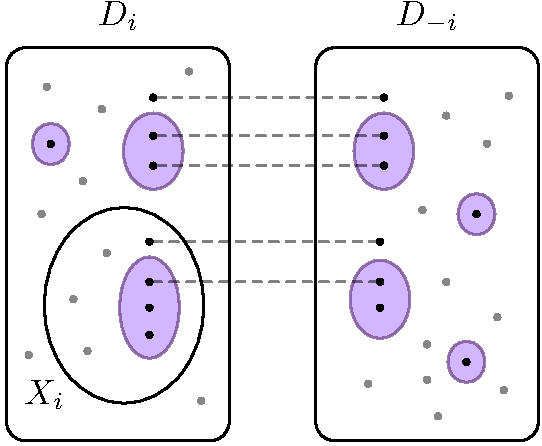
\includegraphics[scale=0.9]{chapter5/fig-efinf.pdf}
%			% \caption{$k=10, n=5, m=2, |S|_{X_i}=3$ and $|S|_{D_i}=|S|_{D_{-i}}=6$.}
%			\caption{Elements of type $S$ have coloured background.}
%			\label{fig:efinf}
%		\end{figure}

		For item~\eqref{it:equiv} we proceed as follows: for every type $S$ such that there is an element $d\in X_i$ of type $S$, we add a new element $d'\in D_{-i}$ of type $S$ to $X_{-i}$. To see that this is always possible, observe first that $\osmodel_0 \sim_k^\infty \osmodel_1$ implies $\osmodel_0 \sim_k^= \osmodel_1$. Using the properties of this relation, we divide in two cases:
		%
		\begin{itemize}
			\item If $|S|_{D_i} \geq k$ we know that $|S|_{D_{-i}} \geq k$ as well. From the elements of $D_{-i}$ of type $S$, at most $n<k$ are used by $f_n$. Hence, there is at least one $d'\in D_{-i}$ of type $S$ to choose from.
			%
			\item If $|S|_{D_i} < k$ we know that $|S|_{D_{i}} = |S|_{D_{-i}}$. From the elements of $D_{i}$ of type $S$, at most $|S|_{D_{i}}-1$ are used by $f_n$. The reason for the $-1$ is that we are assuming that we have just chosen a $d\in X_i$ which is not in $f_n$. Using that $|S|_{D_{i}} = |S|_{D_{-i}}$ and that $f_n$ is a partial isomorphism we can again conclude that there is at least one $d'\in D_{-i}$ of type $S$ to choose from.
		\end{itemize}
		%
		For item~\eqref{it:inf} observe that as $X_{i}$ is infinite but there are only finitely many types, there must be some $S$ such that $|S|_{X_i} \geq \omega$. It is then safe to add infinitely many elements for $S$ in $X_{-i}$ while considering point~\eqref{it:equiv}. Moreover, the existence of infinitely many elements satisfying $S$ in $D_{-i}$ is guaranteed by $\osmodel_0 \sim_k^\infty \osmodel_1$.

		Having shown that \eloise can choose a set $X_{-i}$ satisfying the above conditions, it is now clear that using point~\eqref{it:equiv} \eloise can survive the ``first-order part'' of the second-order move we were considering. This finishes the proof of the claim.
		% we continue the proof of the claim as follows: as $\osmodel_0{\rest}X_0 \sim_{m+1}^= \osmodel_1{\rest}X_1$ and $f':\vlist{r_0}\mapsto\vlist{r_1}$ is a partial isomorphism between them (with sequences of length $m$) then by the first claim of Lemma~\ref{lem:connofoe}, we know that \eloise can survive one round in $\efgame_{m+1}^=(\osmodel_0{\rest}X_0,\osmodel_1{\rest}X_1)@(\vlist{r_0},\vlist{r_1})$. In particular, she can survive the ``first-order part'' of the second-order move we were considering. This finishes the proof of the claim.
	\end{pfclaim}
	%
	Going back to the proof of Lemma~\ref{lem:connolque}, for step~(\ref{lem:connolque:iii}) to~(\ref{lem:connolque:i}) we prove the following.
	%
	\begin{claim}
		Let $\vlist{s_i} \in D_i^n$ and $\varphi(z_1,\dots,z_n) \in \ofoei(A)$ be such that $qr(\varphi) \leq k-n$. If \eloise has a winning strategy in $\efgame_k^\infty(\osmodel_0,\osmodel_1)@(\vlist{s_0},\vlist{s_1})$ then $\osmodel_0 \models \varphi(\vlist{s_0})$ iff $\osmodel_1 \models \varphi(\vlist{s_1})$.
	\end{claim}
	%
	\begin{pfclaim}
		All the cases involving operators of \ofoe are the same as in Lemma~\ref{lem:connofoe}. We prove the inductive case for the generalized quantifier. Let $\varphi(z_1,\dots,z_n)$ be of the form $\qu x.\psi(z_1,\dots,z_n,x)$ and let $\osmodel_0 \models \varphi(\vlist{s_0})$. Hence, there is an \emph{infinite} set $X_0 \subseteq D_0$ such that
		%
		\begin{equation}\label{eq:ind0ok}
		\osmodel_0 \models \psi(\vlist{s_0},x_0) \text{ if and only if } x_0\in X_0 .
		\end{equation}
		%
		By hypothesis we know that \eloise has a winning strategy for $\efgame_k^\infty(\osmodel_0,\osmodel_1)@(\vlist{s_0},\vlist{s_1})$. Therefore, if \abelard plays a second-order move by picking $X_0 \subseteq D_0$ she can respond with some infinite set $X_1 \subseteq D_1$. We claim that $\osmodel_1 \models \psi(\vlist{s_1},x_1)$ for every $x_1\in X_1$. First observe that if this holds then the set $X'_1 := \{ d_1 \in D_1 \mid \osmodel_1 \models \psi(\vlist{s_1},d_1)\}$ must be infinite, and hence $\osmodel_1 \models \qu x.\psi(\vlist{s_1},x)$.% and we are done.
		
		Assume, for a contradiction, that $\osmodel_1 \not\models \psi(\vlist{s_1},x'_1)$ for some $x'_1\in X_1$. Let \abelard play that $x'_1$ as the second part of his move. Then, as \eloise has a winning strategy, she will respond with some $x'_0 \in X_0$ such that she has a winning strategy for $\efgame_{k}^\infty(\osmodel_0,\osmodel_1)@(\vlist{s_0}{\cdot}x'_0,\vlist{s_1}{\cdot}x'_1)$. By induction hypothesis, as $qr(\psi) \leq k-(n+1)$, this means that $\osmodel_0 \models \psi(\vlist{s_0},x'_0)$ iff $\osmodel_1 \models \varphi(\vlist{s_1},x'_1)$ which contradicts~(\ref{eq:ind0ok}). The other direction is symmetric.
	\end{pfclaim}
	%
	Combining the claims finishes the proof of the lemma.
\end{proof}


\begin{theorem}\label{thm:bfofoei}
Every formula $\varphi \in \ofoei(A)$ is equivalent to a formula in basic form.
\end{theorem}
\begin{proof}
	This can be proved using the same technique as in Theorem~\ref{thm:bnfofoe}. Hence we only focus on showing that $\varphi_E^\infty \equiv \dbnfofoei{\vlist{T}}{\Pi}{\Sigma}$ for some $\Pi,\Sigma \subseteq \wp A$ and $T_i \subseteq A$. Recall that
	\[
	\varphi^\infty_E = \varphi^=_{E'} \land \dbnfinf{\{S_1,\dots,S_n\}}
	\]
	where $\{S_1,\dots,S_n\}$ are all the types that should be satisfied by infinitely many elements.
	Using Theorem~\ref{thm:bnfofoe} on $\varphi^=_{E'}$ we know that this is equivalent to
	\[
	\varphi^\infty_E = \dbnfofoe{\vlist{T}'}{\Pi'} \land \dbnfinf{\{S_1,\dots,S_n\}}
	\]
	for some $\Pi' \subseteq \wp A$ and $T'_i \subseteq A$. Now separate $\Pi'$ as $\Pi' = \Pi \uplus \Sigma$ where $\Sigma:=\{S_1,\dots,S_n\}$ is composed of the infinite types and $\Pi := \Pi'\setminus\Sigma$ is composed of the finite types. After a minor rewriting, we get that
	%
	\[
	\varphi^\infty_E \equiv \dbnfofoe{\vlist{T}'}{\Pi\cup\Sigma} \land \dbnfinf{\Sigma}.
	\]
	%
	Therefore, we can conclude that $\varphi^\infty_E \equiv \dbnfofoei{\vlist{T}'}{\Pi}{\Sigma}$.
\end{proof}

\noindent The following stronger normal form will be useful in later chapters.

\begin{proposition}\label{prop:bfofoei-sigmapi}
	For every formula in the basic form $\bigvee \dbnfofoei{\vlist{T}}{\Pi}{\Sigma}$ it is possible to assume, without loss of generality, that $\Sigma \subseteq \Pi$.
\end{proposition}
\begin{proof}
	This is direct from observing that $\dbnfofoei{\vlist{T}}{\Pi}{\Sigma}$ is equivalent to $\dbnfofoei{\vlist{T}}{\Pi\cup\Sigma}{\Sigma}$. To check it we just unravel the definitions and observe that
	$\dbnfofoe{\vlist{T}}{\Pi \cup \Sigma} \land \dbnfinf{\Sigma}$ is equivalent to $\dbnfofoe{\vlist{T}}{\Pi \cup \Sigma \cup \Sigma} \land \dbnfinf{\Sigma}$.
\end{proof}

\subsection{One-step monotonicity}\label{subsec:one-stepmonot}
% !TEX root = ../main.tex

\index{formula!one-step!monotone}
Given a one-step logic $\llang(A)$ and formula $\varphi \in \llang(A)$.
%
We say that $\varphi$ is \emph{monotone in $\{\vlist{a}\} \subseteq A$} if for every one step model $(D,\val)$ and assignment $\ass:\fovar\to D$,
\[
\text{if } (D,\val),\ass \models \varphi \text{ and } \val(\vlist{a}) \subseteq \vlist{E} \text{ then } (D,\val[\vlist{a}\mapsto \vlist{E}]),\ass \models \varphi.
\]
%
% We use $\llang^+(A)$ to denote the fragment of $\llang(A)$ composed of formulas monotone in all $a\in A$.

\begin{remark}\label{rem:monotprodeach}
	It is easy to prove that a formula is monotone in $\{\vlist{a}\} \subseteq A$ iff it is monotone in every $a_i$. Therefore, in the following proofs we will, in general, consider monotonicity in every single $a_i$ instead of in the full $\vlist{a}$. This is equivalent, and only done to avoid an even more complex notation.
\end{remark}

Monotonicity is usually tightly related to positivity. If the quantifiers are well-behaved (i.e., monotone) then a formula $\varphi$ will usually be monotone in $a \in A$ iff $a$ has positive polarity in $\varphi$, that is, if it only occurs under an even number of negations. This is the case for all one-step logics considered in this dissertation. In this section we give a syntactic characterization of monotonicity for several one-step logics.

\index{$\tau^{A'}_S$}
\index{type!$A'$-positive}
\begin{definition}
	Given $S \subseteq A$ and $A' \subseteq A$ we use the following notation
	\[
	\tau^{A'}_S(x) := \bigwedge_{b\in S} b(x) \land \bigwedge_{b\in A\setminus (S\cup A')}\lnot b(x) ,
	\]
	for what we call the \emph{$A'$-positive} $A$-type $\tau^{A'}_S$.
	Intuitively, $\tau^{A'}_S$ works almost like the $A$-type $\tau_S$, but discarding the negative information for the names in $A'$.
	If $A' = \{a\}$ we write $\tau^a_S$ instead of $\tau^{\{a\}}_S$. Observe that with this notation, $\tau^+_S$ is equivalent to $\tau^A_S$.
	%Moreover, we use $\tau^+_S$ to denote the \emph{positive} $A$-type defined as $\tau^+_S(x) := \bigwedge_{b\in S} b(x)$.
\end{definition}

%	For every one-step logic $\llang$ for which we have a basic form based on disjuncts $\dbnf_{\llang}$ we use $\dbnf^p_{\llang}$ to denote the basic form that we get by replacing every type $\tau_S$ with $\tau^a_S$; analogously, we use $\dbnf_{\llang}^+$ to denote the replacement of every type $\tau_S$ with $\tau^+_S$.

%%
\subsubsection{Monotone fragment of $\ofo$}

\index{fragment!monotone!$\ofo$}
\index{$\ofo$!$\monot{}{A'}$}
\begin{theorem}\label{thm:ofomonot}
A formula of $\ofo(A)$ is monotone in $A' \subseteq A$ iff it is equivalent to a sentence given by:
\[
\varphi ::= \psi \mid a(x) \mid \exists x.\varphi \mid \forall x.\varphi \mid \varphi \land \varphi \mid \varphi \lor \varphi
\]
where $a \in A'$,
$\psi \in \ofo(A\setminus A')$. We denote this fragment as $\monot{\ofo}{A'}(A)$.
\end{theorem}
%
The result will follow from the following two lemmas and Remark~\ref{rem:monotprodeach}.

\begin{lemma}\label{lem:monofoismonot}
Every $\varphi \in \monot{\ofo}{a}(A)$ is monotone in $a$.
\end{lemma}
\begin{proof}
	The proof is a routine argument by induction on the complexity of $\varphi$.
\end{proof}
% \begin{proof}
% We show, by induction, that any one-step formula $\varphi$ in the fragment (which may not be a sentence) satisfies, for every one-step model $(D,\val:A\to\wp D)$, assignment ${\ass:\fovar\to D}$, 
% %
% \[(D,\val),\ass \models \varphi \text{ and } \val(a) \subseteq E \text{ then } (D,\val[a\mapsto E]),\ass \models \varphi.\] 
% %
% \begin{enumerate}[\textbullet]
% \item If ${\varphi = \psi \in \ofo(A\setminus \{a\})}$ changes in the $a$ part of the valuation will make no difference and hence the condition is trivial. %The same happens if $\varphi = q(x)$ with $q\in P$ but $q \neq a$.

% \item Case $\varphi = a(x)$: if $(D,\val),\ass \models a(x)$ then $\ass(x)\in \val(a)$. Clearly, $\ass(x) \in \val[a\mapsto E](a)$ because $\val(a) \subseteq E$. Therefore $(D, \val[a\mapsto E]),\ass \models a(x)$. %For the other direction assume $U \subseteq_\omega \val(a)$ and $(D, \val[a\mapsto U]),\ass \models a(x)$. This means that $\ass(x) \in U \subseteq \val(a)$, hence $(D, \val),\ass \models a(x)$.

% \item Case $\varphi = \varphi_1 \lor \varphi_2$: assume $(D,\val),\ass \models \varphi$. Without loss of generality we can assume that $(D,\val),\ass \models \varphi_1$ and hence by induction hypothesis we have that $(D,\val[a\mapsto E]),\ass \models \varphi_1$ which clearly satisfies $(D,\val[a\mapsto E]),\ass \models \varphi$. %For the other direction let $U \subseteq_\omega \val(a)$ and assume wlog that $(D,\val[a\mapsto U]),\ass \models \varphi_1$. By induction hypothesis $(D,\val),\ass \models \varphi_1$ which entails $(D,\val),\ass \models \varphi$.

% \item Case $\varphi = \varphi_1 \land \varphi_2$: assume $(D,\val),\ass \models \varphi$. As we have $(D,\val),\ass \models \varphi_i$, by induction hypothesis we get $(D,\val[a\mapsto E]),\ass \models \varphi_i$. Therefore $(D,\val[a\mapsto E]),\ass \models \varphi$. %The other direction is very similar to the case of disjunction.

% \item Case $\varphi = \exists x.\varphi'(x)$ and $(D,\val),\ass \models \varphi$. By definition there exists $d\in D$ such that $(D,\val),\ass[x\mapsto d] \models \varphi'(x)$. By induction hypothesis $(D,\val[a\mapsto E]),\ass[x\mapsto d] \models \varphi'(x)$ and hence $(D,\val[a\mapsto E]),\ass \models \exists x.\varphi'(x)$.

% \item Case $\varphi = \forall x.\varphi'(x)$ and $(D,\val),\ass \models \varphi$. By definition $(D,\val),\ass[x\mapsto d] \models \varphi'(x)$ for all $d\in D$. By induction hypothesis $(D,\val[a\mapsto E]),\ass[x\mapsto d] \models \varphi'(x)$ for all $d\in D$. Hence $(D,\val[a\mapsto E]),\ass \models \forall x.\varphi'(x)$.
% \end{enumerate}
% %
% This finishes the proof.
% \end{proof}

Before going on we need to introduce a bit of new notation. In Section~\ref{subsec:normalforms} we introduced the formula $\dbnfofo{\Sigma}$. We now give a few variants of this notation, which will be crucial to build the normal forms of the fragments discussed in this dissertation.

\index{$\mondbnfofo{\Sigma}{A'}$}
\index{$\mondgbnfofo{\Sigma}{\Pi}{A'}$}
\begin{definition}
Let $A'\subseteq A$ be a finite set of names. The $A'$-positive variant of $\dbnfofo{\Sigma}$ is given as follows:
% \begin{align*}
% 	\mondbnfofo{\Sigma}{A'} &:= \bigwedge_{S\in\Sigma} \exists x. \tau^{A'}_S(x) \land \forall x. \bigvee_{S\in\Sigma} \tau^{A'}_S(x) \\
% 	\posdbnfofo{\Sigma} &:= \bigwedge_{S\in\Sigma} \exists x. \tau^+_S(x) \land \forall x. \bigvee_{S\in\Sigma} \tau^+_S(x) .
% \end{align*}
\[
	\mondbnfofo{\Sigma}{A'} := \bigwedge_{S\in\Sigma} \exists x. \tau^{A'}_S(x) \land \forall x. \bigvee_{S\in\Sigma} \tau^{A'}_S(x).
\]
We also introduce the following generalized forms of the above notation:
% \begin{align*}
% 	\mondgbnfofo{\Sigma}{\Pi}{A'} &:= \bigwedge_{S\in\Sigma} \exists x. \tau^{A'}_S(x) \land \forall x. \bigvee_{S\in\Pi} \tau^{A'}_S(x) \\
% 	\posdgbnfofo{\Sigma}{\Pi} &:= \bigwedge_{S\in\Sigma} \exists x. \tau^+_S(x) \land \forall x. \bigvee_{S\in\Pi} \tau^+_S(x) .
% \end{align*}
\[
	\mondgbnfofo{\Sigma}{\Pi}{A'} := \bigwedge_{S\in\Sigma} \exists x. \tau^{A'}_S(x) \land \forall x. \bigvee_{S\in\Pi} \tau^{A'}_S(x) .
\]
The \emph{positive} variants of the above notations are defined as $\posdbnfofo{\Sigma} := \mondbnfofo{\Sigma}{A}$ and $\posdgbnfofo{\Sigma}{\Pi} := \mondgbnfofo{\Sigma}{\Pi}{A}$.
\end{definition}

To prove that the fragment $\monot{\ofo}{a}$ is complete for monotonicity in $a$, we need to show that every formula which is monotone in $a$ is equivalent to some formula in $\monot{\ofo}{a}$. We prove a stronger result: we give a translation that constructively maps arbitrary formulas into $\monot{\ofo}{a}$. The interesting observation is that the translation will preserve truth iff the given formula is monotone in $a$.

\begin{lemma}
There exists a translation $(-)^\tmono:\ofo(A) \to \monot{\ofo}{a}(A)$ such that
a formula ${\varphi \in \ofo(A)}$ is monotone in $a\in A$ if and only if $\varphi\equiv \varphi^\tmono$.
\end{lemma}
%
\begin{proof}
To define the translation we assume, without loss of generality, that $\varphi$ is in the normal form $\bigvee \dbnfofo{\Sigma}$ given in Definition~\ref{def:bfofo}, that is:
%
\[
\dbnfofo{\Sigma} := \bigwedge_{S\in\Sigma} \exists x. \tau_S(x) \land \forall x. \bigvee_{S\in\Sigma} \tau_S(x).
\]
%
% for some types $\Sigma \subseteq \wp A$.
%
We define the translation as
$(\bigvee \dbnfofo{\Sigma})^\tmono:= \bigvee \mondbnfofo{\Sigma}{a}$.
%  where
% %
% \[
% \mondbnfofo{\Sigma}{A'} := \bigwedge_{S\in\Sigma} \exists x. \tau^{A'}_S(x) \land \forall x. \bigvee_{S\in\Sigma} \tau^{A'}_S(x)
% \]

From the construction it is clear that $\varphi^\tmono \in \monot{\ofo}{a}(A)$ and therefore the right-to-left direction of the lemma is immediate by Lemma~\ref{lem:monofoismonot}. For the left-to-right direction assume that $\varphi$ is monotone in $a$, we have to prove that $(D,\val) \models \varphi$ if and only if $(D,\val) \models \varphi^\tmono$.

\bigskip
\noindent \fbox{$\Rightarrow$} This direction is trivial.

\bigskip
\noindent \fbox{$\Leftarrow$} Assume $(D,\val) \models \varphi^\tmono$ and let $\Sigma$ be such that $(D,\val) \models \mondbnfofo{\Sigma}{a}$. Because of the universal part of $\mondbnfofo{\Sigma}{a}$, it is safe to assume that the \emph{only} ($a$-positive) types realized in $(D,\val)$ are exactly those in $\Sigma$; moreover, it is also safe to assume that every type has a (single) distinct witness (this is because $(D,\val)$ can be proved to be $\ofo$-equivalent to such a model).
%
%We have to prove that $(D,\val) \models \varphi$. It is easy to prove that $(D,\val) \equiv_\fo (D\times \{0,1\},\val_\pi)$ where $D\times\{0,1\}$ has $2$ copies of each element of $D$ and $\val_\pi((d,i)) := \val(d)$. Hence, it is enough to prove that $(D\times \{0,1\},\val_\pi) \models \varphi$.
%
For every $S \in \Sigma$, let $d_S$ be the witness of the $a$-positive type $\tau^a_S(x)$ in $(D,\val)$. Let $U := \{d_S \mid S\in \Sigma, a\notin S\}$ and $\val' := \val[a \mapsto \val(a) \setminus U]$. 

\begin{claimfirst}
	$(D,\val') \models \dbnfofo{\Sigma}$.
\end{claimfirst}

\begin{pfclaim}
First we show that the existential part of the normal form is satisfied. That is, that for every $S\in \Sigma$ we have a witness for the \emph{full} type $\tau_S(x)$. If $a\in S$ the witness is given by $\varphi^\tmono$, that is, $d_S$. If $a \notin S$ then we specially crafted $d_S$ to be a witness. The universal part is clearly satisfied.
\end{pfclaim}
%
To finish observe that, by monotonicity of $\varphi$, we get $(D,\val) \models \varphi$. %This finishes the proof of the lemma.
\end{proof}

Putting together the above lemmas we obtain Theorem~\ref{thm:ofomonot}. Moreover, a careful analysis of the translation gives us the following corollary, providing normal forms for the monotone fragment of $\ofo$.

\begin{corollary}\label{cor:ofopositivenf} Let $\varphi \in \ofo(A)$, the following hold:
	\begin{enumerate}[(i)]
		\item The formula $\varphi$ is monotone in $A' \subseteq A$ iff it is equivalent to a formula in the basic form $\bigvee \mondbnfofo{\Sigma}{A'}$ for some types $\Sigma \subseteq \wp A$.
		%
		\item The formula $\varphi$ is monotone in every $a\in A$ (i.e., $\varphi\in\ofo^+(A)$) iff $\varphi$ is equivalent to a formula $\bigvee \posdbnfofo{\Sigma}$ for some types $\Sigma \subseteq \wp A$. %, where
		%
		%For the translation, let
		%$(\bigvee \dbnfofo{\Sigma})^\tmono:= \bigvee \mondbnfofo{\Sigma}{a}$ and
		%
		% \[
		% \posdbnfofo{\Sigma} := \bigwedge_{S\in\Sigma} \exists x. \tau^+_S(x) \land \forall x. \bigvee_{S\in\Sigma} \tau^+_S(x) .
		% \]
	\end{enumerate}
\end{corollary}

% The following stronger normal form will be useful. Intuitively, it says that every set $\Sigma$ is comprised of types that are incomparable (in terms of containment) between each other.

% \begin{proposition}\label{props:strongmonofo}
% In the above normal form we can assume that every disjunct $\mondbnfofo{\Sigma}{A'}$ is such that for every pair of distinct $S,S'\in \Sigma$ at least one of the following conditions hold:
% \begin{itemize}
% 	\itemsep 0 pt
% 	\item $S \cap (A\setminus A') \neq S' \cap (A\setminus A')$, or
% 	\item $S \cap A' \not\subseteq S' \cap A'$ and $S' \cap A' \not\subseteq S \cap A'$.
% \end{itemize}
% \end{proposition}
% %
% \begin{proof}
% 	Assume that for some distinct $S,S'\in\Sigma$ neither of the conditions hold. That is,
% 	%
% 	$S \cap (A\setminus A') = S' \cap (A\setminus A')$ and
% 	either (1) $S \cap A' \subseteq S' \cap A'$ or (2) $S' \cap A' \subseteq S \cap A'$.
% 	%
% 	It is easy to observe that if (1) holds then $\tau^{A'}_{S'}(x) \models \tau^{A'}_{S}(x)$ and if (2) holds then $\tau^{A'}_{S}(x) \models \tau^{A'}_{S'}(x)$.

% 	\begin{claimfirst}
% 		In both cases $\mondbnfofo{\Sigma}{A'}\equiv \mondbnfofo{\Sigma\setminus \{S\}}{A'} \lor \mondbnfofo{\Sigma\setminus \{S'\}}{A'}$.
% 	\end{claimfirst}
% 	%
% 	\begin{pfclaim}
% 		We only prove case (1) since the cases are symmetric. Let $(D,\val) \models \mondbnfofo{\Sigma}{A'}$. Either (a) every element satisfying $\tau^{A'}_{S}(x)$ also satisfies $\tau^{A'}_{S'}(x)$ or; (b)~there are witnesses for $\tau^{A'}_{S}(x)$ which do not satisfy $\tau^{A'}_{S'}(x)$. In case~(a) we clearly have that $(D,\val) \models \mondbnfofo{\Sigma\setminus \{S\}}{A'}$. For case~(b), it is trivial to see that $(D,\val)$ satisfies the existential part of $\mondbnfofo{\Sigma\setminus \{S'\}}{A'}$ since it poses less constraints. For the universal part, suppose that some element satisfies $\tau^{A'}_{S'}(x)$, then in particular (by hypothesis) it also satisfies $\tau^{A'}_{S}(x)$. Since $S\in \Sigma\setminus \{S'\}$ this does not carry any problem. We can conclude that $(D,\val) \models \mondbnfofo{\Sigma\setminus \{S'\}}{A'}$.
% 	\end{pfclaim}
% 	%
% 	This finishes the proof.
% \end{proof}

%%
\subsubsection{Monotone fragment of $\ofoe$}

\index{fragment!monotone!$\ofoe$}
\index{$\ofoe$!$\monot{}{A'}$}
\begin{theorem}\label{thm:ofoemonot}
A formula of $\ofoe(A)$ is monotone in ${A'\subseteq A}$ iff it is equivalent to a sentence given by:
\[
\varphi ::= \psi \mid a(x) \mid \exists x.\varphi \mid \forall x.\varphi \mid \varphi \land \varphi \mid \varphi \lor \varphi
\]
where $a\in A'$ and $\psi \in \ofoe(A\setminus A')$. We denote this fragment as $\monot{\ofoe}{A'}(A)$.
\end{theorem}

Observe that, in this definition, the equality predicate is taken into account by the $\psi$ clause.
Before going on we need to introduce a bit of new notation. 

\index{$\mondbnfofoe{\vlist{T}}{\Pi}{A'}$}
\index{$\posdbnfofoe{\vlist{T}}{\Pi}$}
\begin{definition}
Let $A'\subseteq A$ be a finite set of names. The monotone variant of $\dbnfofoe{\vlist{T}}{\Pi}$ is given as follows:
\begin{align*}
	\mondbnfofoe{\vlist{T}}{\Pi}{A'} &:= \exists \vlist{x}.\big(\arediff{\vlist{x}} \land \bigwedge_i \tau^{A'}_{T_i}(x_i) \land \forall z.(\arediff{\vlist{x},z} \lthen \bigvee_{S\in \Pi} \tau^{A'}_S(z))\big). 
	% \\
	% \posdbnfofoe{\vlist{T}}{\Pi} &:= \exists \vlist{x}.\big(\arediff{\vlist{x}} \land \bigwedge_i \tau^{+}_{T_i}(x_i) \land \forall z.(\arediff{\vlist{x},z} \lthen \bigvee_{S\in \Pi} \tau^{+}_S(z))\big) .
\end{align*}
When the set $A'$ is a singleton $\{a\}$ we will write $a$ instead of $A'$. The positive variant of $\dbnfofoe{\vlist{T}}{\Pi}$ is defined as above but with $+$ in place of $A'$.
\end{definition}

\noindent The result follows from the following lemma.

\begin{lemma}
The following hold:
\begin{enumerate}
	\itemsep 0pt
	\item Every $\varphi \in \monot{\ofoe}{A'}(A)$ is monotone in $A'$.
	\item There exists a translation $(-)^\tmono:\ofoe(A) \to \monot{\ofoe}{A'}(A)$ such that
a formula ${\varphi \in \ofoe(A)}$ is monotone in $A'$ if and only if $\varphi\equiv \varphi^\tmono$.
\end{enumerate}
\end{lemma}
\begin{proof}
	In Theorem~\ref{thm:ofoeimonot} this result is proved for \ofoei (i.e., \ofoe extended with generalized quantifiers). It is not difficult to adapt the proof for $\ofoe$. Intuitively, the translation is defined as $\varphi^\tmono := \varphi[\lnot a(x) \mapsto \top \mid a\in A']$ for $\varphi$ in negation normal form.
\end{proof}

Combining the normal form for $\ofoe$ and the above lemma, we obtain the following corollary providing a normal form for the monotone fragment of $\ofoe$.

\begin{corollary}\label{cor:ofoepositivenf}
	Given $\varphi \in \ofoe(A)$, the following hold:
	\begin{enumerate}[(i)]
		\item The formula $\varphi$ is monotone in $A'\subseteq A$ iff it is equivalent to a formula in the basic form $\bigvee \mondbnfofoe{\vlist{T}}{\Pi}{A'}$
		where
		%
		% \[
		% 	\mondbnfofoe{\vlist{T}}{\Pi}{A'} := \exists \vlist{x}.\big(\arediff{\vlist{x}} \land \bigwedge_i \tau^{A'}_{T_i}(x_i) \land \forall z.(\arediff{\vlist{x},z} \lthen \bigvee_{S\in \Pi} \tau^{A'}_S(z))\big)
		% \]
		% and
		for each disjunct we have $\vlist{T} \in \wp(A)^k$ for some $k$ and $\Pi\subseteq\vlist{T}$,
		%
		\item The formula $\varphi$ is monotone in all $a\in A$ (i.e., $\varphi\in \ofoe^+(A)$) iff it is equivalent to a formula in the basic form $\bigvee \posdbnfofoe{\vlist{T}}{\Pi}$
		where
		%
		% \[
		% 	\posdbnfofoe{\vlist{T}}{\Pi} := \exists \vlist{x}.\big(\arediff{\vlist{x}} \land \bigwedge_i \tau^{+}_{T_i}(x_i) \land \forall z.(\arediff{\vlist{x},z} \lthen \bigvee_{S\in \Pi} \tau^{+}_S(z))\big)
		% \]
		% and
		for each disjunct we have $\vlist{T} \in \wp(A)^k$ for some $k$ and $\Pi\subseteq\vlist{T}$.
	\end{enumerate}
\end{corollary}

%%
\subsubsection{Monotone fragment of $\ofoei$}

\index{fragment!monotone!$\ofoei$}
\index{$\ofoei$!$\monot{}{A'}$}
\begin{theorem}\label{thm:ofoeimonot}
A formula of $\ofoei(A)$ is monotone in ${A' \subseteq A}$ iff it is equivalent to a sentence given by:
\[
\varphi ::= \psi \mid a(x) \mid \exists x.\varphi \mid \forall x.\varphi \mid \varphi \land \varphi \mid \varphi \lor \varphi \mid \qu x.\varphi \mid \dqu x.\varphi
\]
where $a\in A'$ and $\psi \in \ofoei(A\setminus A')$. We call this fragment $\monot{\ofoei}{A'}(A)$.
\end{theorem}

Observe that $x \foeq y$ and $x \not\foeq y$ are included in the case $\psi \in \ofoei(A\setminus A')$. The result will follow from the following two lemmas and Remark~\ref{rem:monotprodeach}.

\begin{lemma}\label{lem:monofoeiismonot}
Every $\varphi \in \monot{\ofoei}{a}(A)$ is monotone in $a$.
\end{lemma}
\begin{proof}
The proof is basically the same as Lemma~\ref{lem:monofoismonot}.
That is, we show by induction, that any one-step formula $\varphi$ in the fragment (which may not be a sentence) satisfies, for every one-step model $(D,\val)$ and assignment ${\ass:\fovar\to D}$, 
%
\[
\text{if } (D,\val),\ass \models \varphi \text{ and } \val(a) \subseteq E \text{ then } (D,\val[a\mapsto E]),\ass \models \varphi.
\] 
%
We focus on the generalized quantifiers. Let $(D,\val),\ass \models \varphi$ and $\val(a) \subseteq E$.
%
\begin{enumerate}[\textbullet]
\item Case $\varphi = \qu x.\varphi'(x)$. By definition there exists an infinite set $I\subseteq D$ such that for all $d\in I$ we have $(D,\val),\ass[x\mapsto d] \models \varphi'(x)$. By induction hypothesis $(D,\val[a\mapsto E]),\ass[x\mapsto d] \models \varphi'(x)$ for all $d \in I$. Therefore $(D,\val[a\mapsto E]),\ass \models \qu x.\varphi'(x)$.

\item Case $\varphi = \dqu x.\varphi'(x)$. Hence there exists $I\subseteq D$ such that for all $d\in I$ we have $(D,\val),\ass[x\mapsto d] \models \varphi'(x)$ and $D\setminus I$ is \emph{finite}. By induction hypothesis $(D,\val[a\mapsto E]),\ass[x\mapsto d] \models \varphi'(x)$ for all $d \in I$. Therefore $(D,\val[a\mapsto E]),\ass \models \dqu x.\varphi'(x)$.
\end{enumerate}
%
This finishes the proof.
\end{proof}

\noindent Before going on, we introduce some notation.

\index{$\mondbnfofoei{\vlist{T}}{\Pi}{\Sigma}{A'}$}
\index{$\mondbnfinf{\Sigma}{A'}$}
\index{$\posdbnfofoei{\vlist{T}}{\Pi}{\Sigma}$}
\begin{definition}
Let $A'\subseteq A$ be a finite set of names. The $A'$-positive variant of $\dbnfofoei{\vlist{T}}{\Pi}{\Sigma}$ is given as follows:
\begin{align*}
	\mondbnfofoei{\vlist{T}}{\Pi}{\Sigma}{A'} &:= \mondbnfofoe{\vlist{T}}{\Pi \cup \Sigma}{A'} \land \mondbnfinf{\Sigma}{A'}\\
	%
	\mondbnfofoe{\vlist{T}}{\Lambda}{A'} &:= \exists \vlist{x}.\big(\arediff{\vlist{x}} \land \bigwedge_i \tau^{A'}_{T_i}(x_i) \land \forall z.(\arediff{\vlist{x},z} \lthen \bigvee_{S\in \Lambda} \tau^{A'}_S(z))\big) \\
	%
	\mondbnfinf{\Sigma}{A'} &:= \bigwedge_{S\in\Sigma} \qu y.\tau^{A'}_S(y) \land \dqu y.\bigvee_{S\in\Sigma} \tau^{A'}_S(y) .
\end{align*}
When the set $A'$ is a singleton $\{a\}$ we will write $a$ instead of $A'$. The positive variant of $\dbnfofoei{\vlist{T}}{\Pi}{\Sigma}$ is defined as $\posdbnfofoei{\vlist{T}}{\Pi}{\Sigma} := \mondbnfofoei{\vlist{T}}{\Pi}{\Sigma}{A}$.
\end{definition}

\noindent We are now ready to give the translation.

\begin{lemma}
There is a translation $(-)^\tmono:\ofoei(A) \to \monot{\ofoei}{a}(A)$ such that
a formula ${\varphi \in \ofoei(A)}$ is monotone in $a$ if and only if $\varphi\equiv \varphi^\tmono$.
\end{lemma}
\begin{proof}
We assume that $\varphi$ is in the normal form $\bigvee \dbnfofoei{\vlist{T}}{\Pi}{\Sigma}$ where 
%
\[
\dbnfofoei{\vlist{T}}{\Pi}{\Sigma} = \dbnfofoe{\vlist{T}}{\Pi \cup \Sigma} \land \dbnfinf{\Sigma} .
\]
%
for some sets of types $\Pi,\Sigma \subseteq \wp A$ and each $T_i \subseteq A$.
%
For the translation we define
\[
(\bigvee \dbnfofoei{\vlist{T}}{\Pi}{\Sigma})^\tmono:= \bigvee \mondbnfofoei{\vlist{T}}{\Pi}{\Sigma}{a}.
\]
%
From the construction it is clear that $\varphi^\tmono \in \monot{\ofoei}{a}(A)$ and therefore the right-to-left direction of the lemma is immediate by Lemma~\ref{lem:monofoeiismonot}. For the left-to-right direction assume that $\varphi$ is monotone in $a$, we have to prove that $(D,\val) \models \varphi$ if and only if $(D,\val) \models \varphi^\tmono$.

\bigskip
\noindent \fbox{$\Rightarrow$} This direction is trivial.

\bigskip
\noindent \fbox{$\Leftarrow$}
Assume $(D,\val) \models \varphi^\tmono$, and in particular that $(D,\val) \models \mondbnfofoei{\vlist{T}}{\Pi}{\Sigma}{a}$.
Observe that the elements of $D$ can be partitioned in the following way:
%
\begin{enumerate}[(a)]
	\itemsep 0 pt
	\item Distinct elements $t_i \in D$ such that each $t_i$ satisfies $\tau^{a}_{T_i}(x)$,% witnessing the $a$-positive type $T_i \in \vlist{T}$,
	\item\label{it:dpi} Disjoint sets $\compset{D_S \subseteq D \mid S \in \Sigma}$ such that each $D_S$ is \emph{infinite} and every $d \in D_S$ is a witness for the $a$-positive type $S \in \Sigma$,
	\item\label{it:ds} A \emph{finite} set $D_\Pi \subseteq D$ of witnesses of the $a$-positive types in $\Pi$.
\end{enumerate}
%
Following this partition, every element $d\in D$ is be the witness of an $a$-type in either (a)~$\vlist{T}$, (b)~$\Sigma$, or (c)~$\Pi$. We use $S_d \in \vlist{T}\cup \Pi \cup \Sigma$ to denote the $a$-type which $d$ witnesses. Now, we are talking about $a$-types, there might be a slight difference between $S_d$ and the actual type that each $d$ has (namely $\val^\natural(d)$). That is, it could be that $d\in\val(a)$ but that $a\notin S_d$. What we want to do now is to shrink $\val$ in such a way that the witnessed ($S_d$) type and the actual type coincide. We give a new valuation $\uval$ defined as $\uval^\natural(d) := S_d$.\footnote{Recall that a valuation $\uval:A\to\wp \osmoddom$ can also be represented as a marking $\uval^\natural: \osmoddom\to\wp A$ given by $\uval^\natural(d) := \{a \in A \mid d\in \val(a)\}$.} Observe that $\uval(a) \subseteq \val(a)$ and $\uval(b) = \val(b)$ for $b\in A\setminus\{a\}$.
%
\begin{claimfirst}
	$(D,\uval) \models \varphi$.
\end{claimfirst}
%
\begin{pfclaim}
	First we check that $(D,\uval) \models \dbnfofoe{\vlist{T}}{\Pi \cup \Sigma}$. It is easy to see that the elements $t_i$ work as witnesses for the \emph{full} types $T_i$. That is $(D,\uval) \models \tau_{T_i}(t_i)$ for every $i$. To prove the universal part of the formula it is enough to show that:
	%
	\begin{enumerate}
		\itemsep 0 pt
		\item Every element $d\in D_\Pi$ realizes the full type $S_d \in \Pi$,
		\item For all $S\in \Sigma$, every element of $D_S$ realizes the full type $S$.
	\end{enumerate}
	%
	Let $d$ be an element of either $D_\Pi$ or any of the $D_S$. By~\eqref{it:dpi} and~\eqref{it:ds} we know $(D,\val) \models \tau_{S_d}^a(d)$. If $a\in S_d$ we can trivially conclude $(D,\uval) \models \tau_{S_d}(d)$. If $a\notin S_d$, by definition of $\uval$ we know that $d \notin \uval(a)$ and hence we can also conclude that $(D,\uval) \models \tau_{S_d}(d)$.

	To prove that $(D,\uval) \models \bigwedge_{S\in\Sigma} \qu y.\tau_S(y) \land \dqu y.\bigvee_{S\in\Sigma} \tau_S(y)$ we only need to observe that the existential part is satisfied because each $D_S$ is infinite by~\eqref{it:ds} and the universal part is satisfied because the set $D_\Pi \cup \vlist{T}$ is finite by~\eqref{it:dpi}.
\end{pfclaim}
%
To finish the proof, note that by monotonicity of $\varphi$ we get $(D,\val) \models \varphi$.
%
% \begin{itemize}
% 	\itemsep 0 pt
% 	\item $(D,\val') \models \varphi^\tmono$,
% 	\item $\val'(a) \subseteq \val(a)$ and $\val'(b) = \val(b)$ for all $b\in A\setminus\{a\}$,
% 	\item For every $W \subset \val'(a)$ we have $(D,\val'[a\mapsto W]) \not\models \varphi^\tmono$.
% \end{itemize}
% %
% We prove that $(D,\val') \models \varphi$ and by monotonicity we get $(D,\val) \models \varphi$.
% Let $\vlist{d}$ be the sequence of pairwise distinct elements of $D$
% witnessing the types $\vlist{T}$ in $\mondbnfofoe{\vlist{T}}{\Pi \cup \Sigma}{a}$.
% %making $\arediff{\vlist{x}} \land \bigwedge_i \tau^a_{T_i}(x_i)  \land \forall z.(\arediff{\vlist{x},z} \lthen \bigvee_{S\in \Sigma \cup \Pi} \tau^a_S(z))$ true. Now, we modify $\val$ as follows. We state that $\val_1|_{D\setminus \vlist{d}}=\val|_{D\setminus \vlist{d}}$, while over $d_i \in \vlist{d}$ it is defined by
% % \[
% % \val_1(d_i)= \begin{cases}
% % \val(d_i) & \text{if } a \in T_i \\
% % \val(d_i) \setminus \{a\} & \text{else.} 
% % \end{cases}
% % \]
% % This means that 
% % \begin{equation}\label{eq:start}
% % (D,\val_1) \models \tau_{T_i}(d_i).
% %  \end{equation}
% % Now, we have that 
% %
% % \begin{claimfirst}\label{eq:1}
% % 	$(D\setminus \vlist{d},\val) \models  \forall z.\bigvee_{S\in \Sigma\cup\Pi} \tau^a_S(z) \land \bigwedge_{S\in\Sigma} \qu y.\tau^a_S(y) \land \dqu y.\bigvee_{S\in\Sigma} \tau^a_S(y)$.
% % \end{claimfirst}
% % %
% % \begin{pfclaim}
% % 	Prove.
% % \end{pfclaim}
%
% % \begin{equation}\label{eq:1}
% % (D\setminus \vlist{d},\val_1) \models  \forall z.\bigvee_{S\in \Sigma\cup\Pi} \tau^a_S(z)\land
% % \bigwedge_{S\in\Sigma} \qu y.\tau^a_S(y) \land \dqu y.\bigvee_{S\in\Sigma} \tau^a_S(y).
% % \end{equation}
%
% Let $D_\Pi= \{ d' \in D\setminus \vlist{d} \mid (D\setminus \vlist{d}, \val) \not\models \tau^a_S(d'), \forall S\in \Sigma\}$, and $D_\Sigma = D\setminus (\vlist{d} \cup D_\Pi)$. 
% By (\ref{eq:1}), $D_\Pi$ is finite and therefore it holds that
% \begin{equation}\label{eq:2}
% (D_\Sigma, \val_1)\models \forall z.\bigvee_{S\in \Sigma} \tau^a_S(z)\land
% \bigwedge_{S\in\Sigma} \qu y.\tau^a_S(y) \land \dqu y.\bigvee_{S\in\Sigma} \tau^a_S(y).
% \end{equation}
% Let $(D_S : S \in \Sigma)$ be a partition of $D_\Sigma$ such that, for each $D_S$:
% \begin{enumerate}
% \item $D_S$ is infinite, and
% \item $(D,\val) \models  \tau^a_S(d)$, for every $d \in D_S$. 
% \end{enumerate}
% We modify $\val_1$ by stating that $\val_2|_{ \vlist{d}}=\val_1|_{\vlist{d}}$, while over $d' \in D\setminus \vlist{d},$ $\val_2$ is defined as follows. If $d' \in D_\Sigma$, then there is an unique $S\in \Sigma$ such that $d' \in D_S$. Thence
% \[
% \val_2(d')= \begin{cases}
% \val(d') & \text{if } a \in S \\
% \val(d') \setminus \{a\} & \text{else.} 
% \end{cases}
% \]
% If $d' \in D_\Pi$, then let $S_1, \dots, S_\ell$ be the list of all types in $\Pi$ such that  $(D,\val) \models  \tau^a_{S_k}(d')$. Thus
% \[
% \val_2(d')= \begin{cases}
% \val(d') & \text{if } a \in S_1 \cup \dots \cup S_\ell \\
% \val(d') \setminus \{a\} & \text{else.} 
% \end{cases}
% \]
% By construction, we have that the following two facts hold:
%  \begin{itemize}
% \item $(D, \val_2) \models \bigvee_{S\in \Pi} \tau_S(d)$,
%  for each $d \in D_\Pi$, 
%  \item $(D, \val_2) \models \tau_S(d)$, for each $S \in \Sigma$ and $d \in D_S$. 
% \end{itemize}
% In particular, this means that 
% $(D, \val_2) \models \bigvee_{S\in \Sigma\cup\Pi} \tau_S(d),
% \text{ for each }d \in D_\Sigma \cup D_\Pi.
% $
% Thus, since $D_\Pi$ was chosen to be finite and each $D_S$ is infinite, for $S \in \Sigma$,
% \begin{equation}\label{eq:3}
% (D\setminus \vlist{d}, \val_2) \models \forall z.\bigvee_{S\in \Sigma\cup\Pi} \tau_S(z)\land
% \bigwedge_{S\in\Sigma} \qu y.\tau_S(y) \land \dqu y.\bigvee_{S\in\Sigma} \tau_S(y).
% \end{equation}
%  By (\ref{eq:start}) and (\ref{eq:3}) and the fact that $\val_2|_{ \vlist{d}}=\val_1|_{\vlist{d}}$, we have that $(D, \val_2) \models \varphi$.
% Now, notice that $\val_2(a) \subseteq \val(a)$ and $\val_1(a)=\val(a)$, for each $a \in A\setminus \{a\}$. By monotonicity of $\varphi$ in $a$ we can conclude that $(D, V) \models \varphi$.
\end{proof}

Putting together the above lemmas we obtain Theorem~\ref{thm:ofoeimonot}. Moreover, a careful analysis of the translation gives us the following corollary, providing normal forms for the monotone fragment of $\ofoei$.

\begin{corollary}\label{cor:ofoeipositivenf}
	Let $\varphi \in \ofoei(A)$, the following hold:
	\begin{enumerate}[(i)]
		\item The formula $\varphi$ is monotone in $A' \subseteq A$ iff it is equivalent to a formula $\bigvee \mondbnfofoei{\vlist{T}}{\Pi}{\Sigma}{A'}$ for $\Sigma\subseteq\Pi \subseteq \wp A$ and $\vlist{T} \in \wp(A)^k$ for some $k$.
		%
		\item The formula $\varphi$ is monotone in every $a\in A$ (i.e., $\varphi\in{\ofoei}^+(A)$) iff it is equivalent to a formula in the basic form $\bigvee \posdbnfofoei{\vlist{T}}{\Pi}{\Sigma}$ for types $\Sigma\subseteq\Pi \subseteq \wp A$ and $\vlist{T} \in \wp(A)^k$ for some $k$.
		% , where
		% %
		% %For the translation, let
		% %$(\bigvee \dbnfofo{\Sigma})^\tmono:= \bigvee \mondbnfofo{\Sigma}{a}$ and
		% %
		% \begin{align*}
		% 	\posdbnfofoei{\vlist{T}}{\Pi}{\Sigma} :=\ & \mondbnfofoe{\vlist{T}}{\Pi \cup \Sigma}{+} \land \posdbnfinf{\Sigma} \\
		% 	%
		% 	\posdbnfofoe{\vlist{T}}{\Lambda} :=\ & \exists \vlist{x}.\big(\arediff{\vlist{x}} \land \bigwedge_i \tau^+_{T_i}(x_i) \land \forall z.(\arediff{\vlist{x},z} \lthen \bigvee_{S\in \Lambda} \tau^+_S(z))\big) \\
		% 	%
		% 	\posdbnfinf{\Sigma} :=\ & \bigwedge_{S\in\Sigma} \qu y.\tau^+_S(y) \land \dqu y.\bigvee_{S\in\Sigma} \tau^+_S(y) .
		% \end{align*}
		% %for some types $\Pi,\Sigma \subseteq \wp A$ and $T_i \subseteq A$.
	\end{enumerate}
	%
\end{corollary}
\begin{proof}
	We only remark that to obtain $\Sigma\subseteq\Pi$ in the above normal forms it is enough to use Proposition~\ref{prop:bfofoei-sigmapi} before applying the translation.
\end{proof}

\subsection{One-step continuity}\label{subsec:one-stepcont}
% !TEX root = ../main.tex

Recall from Chapter~\ref{chap:sub} that a formula $\varphi \in \llang(A)$ is continuous in $\{\vlist{a}\} \subseteq A$ if $\varphi$ is monotone in $\vlist{a}$ and additionally, for every $(D,\val)$ and assignment $\ass:\fovar\to D$,
\[
\text{if } (D,\val),\ass \models \varphi \text{ then } \exists \vlist{U} \subseteq_\omega \val(\vlist{a}) \text{ such that } (D, \val[\vlist{a} \mapsto \vlist{U}]),\ass \models \varphi.
\]

\begin{remark}\label{rem:contprodeach}
	It was proved in Proposition~\ref{prop:contiffpcont} that continuity in the product coincides with continuity in every variable. Therefore, in the following proofs we will, in general, consider continuity in every single $a_i$ instead of in the full $\vlist{a}$. This is equivalent, and only done to avoid an even more complex notation.
\end{remark}

In this section we will characterize the continuous fragment of $\ofo$ and $\ofoei$ but we will not characterize that of $\ofoe$, since it is not used in this dissertation.
% It will be useful to give a syntactic characterization of continuity for several one-step logics.

%%
\subsubsection{Continuous fragment of $\ofo$}

\index{fragment!continuous!$\ofo$}
\index{$\ofo$!$\cont{}{A'}$}
\begin{theorem}\label{thm:ofocont}
A formula of $\ofo(A)$ is continuous in $A' \subseteq A$ iff it is equivalent to a sentence given by:
\[
\varphi ::= \psi \mid a(x) \mid \exists x.\varphi \mid \varphi \land \varphi \mid \varphi \lor \varphi
\]
where $a\in A'$ and $\psi \in \ofo(A\setminus A')$. We denote this fragment as $\cont{\ofo}{A'}(A)$.
\end{theorem}
%
The theorem will follow from the next two lemmas and Remark~\ref{rem:contprodeach}.

\begin{lemma}\label{lem:cofoiscont}
Every $\varphi \in \cont{\ofo}{a}(A)$ is continuous in $a$.
\end{lemma}
\begin{proof}
First observe that $\varphi$ is monotone in $a$ by Theorem~\ref{thm:ofomonot}.
We show, by induction, that any one-step formula $\varphi$ in the fragment (which may not be a sentence) satisfies, for every one-step model $(D,\val)$, assignment ${\ass:\fovar\to D}$,
%
\[
\text{if } (D,\val),\ass \models \varphi \text{ then } \exists U \subseteq_\omega \val(a) \text{ such that } (D,\val[a\mapsto U]),\ass \models \varphi.
\]
%
\begin{enumerate}[\textbullet]
\item If ${\varphi = \psi \in \ofo(A\setminus \{a\})}$ changes in the $a$ part of the valuation will make no difference and hence the condition is trivial. 

\item Case $\varphi = a(x)$: if $(D,\val),\ass \models a(x)$ then $\ass(x)\in \val(a)$. Clearly, $\ass(x) \in \val[a\mapsto \{\ass(x)\}](a)$ and hence $(D, \val[a\mapsto \{\ass(x)\}]),\ass \models a(x)$. %For the other direction assume $U \subseteq_\omega \val(a)$ and $(D, \val[a\mapsto U]),\ass \models a(x)$. This means that $\ass(x) \in U \subseteq \val(a)$, hence $(D, \val),\ass \models a(x)$.

\item Case $\varphi = \varphi_1 \lor \varphi_2$: assume $(D,\val),\ass \models \varphi$. Without loss of generality we can assume that $(D,\val),\ass \models \varphi_1$ and hence by induction hypothesis we have that there is $U \subseteq_\omega \val(a)$ such that $(D,\val[a\mapsto U]),\ass \models \varphi_1$ which clearly implies $(D,\val[a\mapsto U]),\ass \models \varphi$. %For the other direction let $U \subseteq_\omega \val(a)$ and assume wlog that $(D,\val[a\mapsto U]),\ass \models \varphi_1$. By induction hypothesis $(D,\val),\ass \models \varphi_1$ which entails $(D,\val),\ass \models \varphi$.

\item Case $\varphi = \varphi_1 \land \varphi_2$: assume $(D,\val),\ass \models \varphi$. By induction hypothesis we have $U_1,U_2 \subseteq_\omega \val(a)$ such that $(D,\val[a\mapsto U_1]),\ass \models \varphi_1$ and $(D,\val[a\mapsto U_2]),\ass \models \varphi_2$. By monotonicity this also holds with $\val[a\mapsto U_1 \cup U_2]$ and therefore $(D,\val[a\mapsto U_1 \cup U_2]),\ass \models \varphi$. %The other direction is very similar to the case of disjunction.

\item Case $\varphi = \exists x.\varphi'(x)$ and $(D,\val),\ass \models \varphi$. By definition there exists $d\in D$ such that $(D,\val),\ass[x\mapsto d] \models \varphi'(x)$. By induction hypothesis there exists $U \subseteq_\omega \val(a)$ such that $(D,\val[a\mapsto U]),\ass[x\mapsto d] \models \varphi'(x)$ and hence $(D,\val[a\mapsto U]),\ass \models \exists x.\varphi'(x)$.
% \item Case $\varphi = \exists x.\varphi'(x)$ and $(D,\val),\ass \models \varphi$. This occurs iff there exists $d\in D$ such that $(D,\val),\ass[x\mapsto d] \models \varphi'(x)$. By induction hypothesis this is equivalent to $\exists U \subseteq_\omega \val(a)$ such that $(D,\val[a\mapsto U]),\ass[x\mapsto d] \models \varphi'(x)$ which holds iff $(D,\val[a\mapsto U]),\ass \models \exists x.\varphi'(x)$.
\end{enumerate}
This finishes the proof.
\end{proof}

\begin{lemma}
There is a translation $(-)^\tcont:\monot{\ofo}{a}(A) \to \cont{\ofo}{a}(A)$ such that
a formula ${\varphi \in \monot{\ofo}{a}(A)}$ is continuous in $a$ if and only if $\varphi\equiv \varphi^\tcont$.
\end{lemma}
\begin{proof}
To define the translation we assume, without loss of generality, that $\varphi$ is in the basic form $\bigvee \mondbnfofo{\Sigma}{a}$.
% where
% %
% \[
% \mondbnfofo{\Sigma}{a} := \bigwedge_{S\in\Sigma} \exists x. \tau^a_S(x) \land \forall x. \bigvee_{S\in\Sigma} \tau^a_S(x).
% \]
%
For the translation, let
$(\bigvee \mondbnfofo{\Sigma}{a})^\tcont := \bigvee \mondgbnfofo{\Sigma}{\Sigma^{-}_{a}}{a}$
where
%
% \[
% \mondgbnfofo{\Sigma}{\Pi}{a} := \bigwedge_{S\in\Sigma} \exists x. \tau^a_S(x) \land \forall x. \bigvee_{S\in\Pi} \tau^a_S(x)
% \]
%
% and
$\Sigma^{-}_{a} := \{S\in \Sigma \mid a\notin S\}$.
%Intuitively, the translation says that we should be able to divide the description given by $\dbnfofo{\Sigma}$ in two parts: (1) $\nabla^{-}_p(\Gamma)$ gives a complete (existential and universal) description with respect to colours which are not $a$ and (2) an existential description where $a$ can only appear as a positive constraint.

\bigskip
From the construction it is clear that $\varphi^\tcont \in \cont{\ofo}{a}(A)$ and therefore the right-to-left direction of the lemma is immediate by Lemma~\ref{lem:cofoiscont}. For the left-to-right direction assume that $\varphi$ is continuous in $a$, we have to prove that $(D,\val) \models \varphi$ iff $(D,\val) \models \varphi^\tcont$, for every one-step model $(D,\val)$. We will take a slightly different but equivalent approach.

It is easy to prove that $(D,\val) \equiv_\fo (D\times \omega,\val_\pi)$ where $D\times\omega$ has countably many copies of each element in $D$ and $\val_\pi(a) := \{(d,k) \mid d\in \val(a), k\in\omega\}$.
%
Moreover, as $\varphi$ is continuous in $a$ there is $U \subseteq_\omega \val_\pi(a)$ such that $\val'_\pi := \val[a \mapsto U]$ satisfies $(D\times\omega,\val_\pi) \models \varphi$ iff $(D\times\omega,\val'_\pi) \models \varphi$.
%
Therefore, it is enough to prove that $(D\times\omega,\val'_\pi) \models \varphi$ iff $(D\times\omega,\val'_\pi) \models \varphi^\tcont$. % Assume again that $\varphi = \bigvee \dbnfofo{\Sigma}$.

\bigskip
\noindent \fbox{$\Rightarrow$}
Let $(D\times\omega,\val'_\pi) \models \mondbnfofo{\Sigma}{a}$, we show that $(D\times\omega,\val'_\pi) \models \mondgbnfofo{\Sigma}{\Sigma^{-}_{a}}{a}$. The existential part of $\mondgbnfofo{\Sigma}{\Sigma^{-}_{a}}{a}$ is trivially true. We have to show that every element of $(D\times\omega,\val'_\pi)$ realizes an $a$-positive type in $\Sigma^{-}_{a}$. Take $(d,k) \in D\times\omega$ and let $T$ be the (full) type of $(d,k)$. If $a\notin T$ then trivially $T\in \Sigma^{-}_{a}$ and we are done. Suppose $a\in T$. Observe that in $D\times\omega$ we have infinitely many copies of $d\in D$. However, as $\val'_\pi(a)$ is finite, there must be some $(d,k')$ with type $T' := T\setminus\{a\}$.
%\fcwarning{Write better}
For $\mondbnfofo{\Sigma}{a}$ to be true we must have $T'\in \Sigma$ and hence $T'\in \Sigma^{-}_{a}$. It is easy to see that $(d,k)$ realizes the $a$-positive type $T'$.

\bigskip
\noindent \fbox{$\Leftarrow$}
Let $(D\times\omega,\val'_\pi) \models \mondgbnfofo{\Sigma}{\Sigma^{-}_{a}}{a}$, we show that $(D\times\omega,\val'_\pi) \models \mondbnfofo{\Sigma}{a}$. The existential part is trivial. For the universal part just observe that $\Sigma^{-}_{a} \subseteq \Sigma$.
\end{proof}

Putting together the above lemmas we obtain Theorem~\ref{thm:ofocont}. Moreover, a careful analysis of the translation gives us the following corollary, providing normal forms for the continuous fragment of $\ofo$.

\begin{corollary}\label{cor:ofocontinuousnf}
	Let $\varphi \in \ofo(A)$, the following hold:
	\begin{enumerate}[(i)]
		\item The formula $\varphi$ is continuous in $a \in A$ iff it is equivalent to a formula $\bigvee \mondgbnfofo{\Sigma}{\Sigma^{-}_{a}}{a}$ for some types $\Sigma \subseteq \wp A$, where $\Sigma^{-}_{a} := \{S\in \Sigma \mid a\notin S\}$.
		%
		\item If $\varphi$ is monotone in $A$ (i.e., $\varphi\in\ofo^+(A)$) then $\varphi$ is continuous in $a \in A$ iff it is equivalent to a formula in the basic form $\bigvee \posdgbnfofo{\Sigma}{\Sigma^{-}_{a}}$ for some types $\Sigma \subseteq \wp A$, where $\Sigma^{-}_{a} := \{S\in \Sigma \mid a\notin S\}$.
	\end{enumerate}
\end{corollary}

%%
\subsubsection{Continuous fragment of $\ofoei$}

\index{fragment!continuous!$\ofoei$}
\index{$\ofoei$!$\cont{}{A'}$}
\begin{theorem}\label{thm:ofoeicont}
A formula of $\ofoei(A)$ is continuous in $ A' \subseteq A$ iff it is equivalent to a sentence given by:
\[
\varphi ::= \psi \mid a(x) \mid \exists x.\varphi \mid \varphi \land \varphi \mid \varphi \lor \varphi \mid \wqu x.(\varphi,\psi)
\]
where $a\in A'$ and $\psi \in \ofoei(A\setminus A')$. Recall from Definition~\ref{def:contmufoei} that $\wqu x.(\varphi,\psi)$ is defined as $\forall x.(\varphi(x) \lor \psi(x)) \land \dqu x.\psi(x)$. We denote this fragment as $\cont{\ofoei}{A'}(A)$.
\end{theorem}

\noindent The theorem will follow from the next two lemmas and Remark~\ref{rem:contprodeach}.

\begin{lemma}\label{lem:cofoeiiscont}
Every $\varphi \in \cont{\ofoei}{a}(A)$ is continuous in $a$.
\end{lemma}
\begin{proof}
Observe that monotonicity of $\varphi$ is guaranteed by Theorem~\ref{thm:ofoeimonot}.
We show, by induction, that any formula of the fragment (which may not be a sentence) satisfies, for every one-step model $(D,\val)$ and assignment ${\ass:\fovar\to D}$,
%
\[
\text{if } (D,\val),\ass \models \varphi \text{ then } \exists U \subseteq_\omega \val(a) \text{ such that } (D,\val[a\mapsto U]),\ass \models \varphi.
\]
%
We focus on the inductive case of the new quantifier. Let $\varphi' = \wqu x.(\varphi,\psi)$, i.e., %In other words,
%
\[\varphi' = \forall x.\underbrace{(\varphi(x) \lor \psi(x))}_{\alpha(x)} \land \underbrace{\dqu x.\psi(x)}_\beta.\]
%
Let $(D,\val),\ass \models \varphi'$. By induction hypothesis,
for every $\ass_d := \ass[x\mapsto d]$ which satisfies $(D,\val),\ass_d \models \alpha(x)$ there is $U_d \subseteq_\omega \val(a)$ such that $(D,\val[a\mapsto U_d]),\ass_d \models \alpha(x)$. The crucial observation is that because of $\beta$, %part of $\varphi'$ we know that
only finitely many elements of $d$ make $\psi(d)$ false. Let $U := \bigcup \{U_d \mid (D,\val), \ass_d \not\models \psi(x) \}$. Note that $U$ is a finite union of finite sets, hence finite.
%
\begin{claimfirst}
	Let $\val_U := \val[a\mapsto U]$; then we have $(D,\val_U),\ass \models \varphi'$.
\end{claimfirst}
%
\begin{pfclaim}
	It is clear that $(D,\val_U),\ass \models \beta$ because $\psi$ is $a$-free. To show that the first conjunct is true we have to show that $(D,\val_U),\ass_d \models \varphi(x) \lor \psi(x)$ for every $d\in D$. We consider two cases: (i) if $(D,\val),\ass_d \models \psi(x)$ we are done, again because $\psi$ is $a$-free; (ii) if the former is not the case then $U_d \subseteq U$; moreover, we knew that $(D,\val[a\mapsto U_d]),\ass_d \models \alpha(x)$ and by monotonicity of $\alpha(x)$ we can conclude that $(D,\val_U),\ass_d \models \alpha(x)$.
\end{pfclaim}
%
This finishes the proof of the lemma.
\end{proof}



\begin{lemma}\label{lem:ofoeictrans}
	There is a translation $(-)^\tcont:\monot{\ofoei}{a}(A) \to \cont{\ofoei}{a}(A)$ such that
a formula $\varphi \in \monot{\ofoei}{a}(A)$ is continuous in $a$ if and only if $\varphi\equiv \varphi^\tcont$.
\end{lemma}
\begin{proof} We assume that $\varphi$ is in basic normal form, i.e., $\varphi = \bigvee \mondbnfofoei{\vlist{T}}{\Pi}{\Sigma}{a}$.
% where
% \[
% \mondbnfofoei{\vlist{T}}{\Pi}{\Sigma}{a} = \mondbnfoe{\vlist{T}}{\Pi \cup \Sigma}{a} \land
% \bigwedge_{S\in\Sigma} \qu y.\tau^a_S(y) \land \dqu y.\bigvee_{S\in\Sigma} \tau^a_S(y) .
% \]
For the translation let $(\bigvee \mondbnfofoei{\vlist{T}}{\Pi}{\Sigma}{a})^\tcont := \bigvee \mondbnfofoei{\vlist{T}}{\Pi}{\Sigma}{a}^\tcont$ where
\[
\mondbnfofoei{\vlist{T}}{\Pi}{\Sigma}{a}^\tcont :=
\begin{cases}
	\bot &\text{ if } a\in \bigcup \Sigma\\
	\mondbnfofoei{\vlist{T}}{\Pi}{\Sigma}{a} &\text{ otherwise}.
\end{cases}
\]

First we prove the right-to-left direction of the lemma. By Lemma~\ref{lem:cofoeiiscont} it is enough to show that $\varphi^\tcont \in \cont{\ofoei}{a}(A)$. We focus on the disjuncts of $\varphi^\tcont$. The interesting case is when $a\notin \bigcup \Sigma$. If we rearrange $\mondbnfofoei{\vlist{T}}{\Pi}{\Sigma}{a}$ and define the formulas $\varphi', \psi$ as follows:
%
\begin{align*}
\mondbnfofoei{\vlist{T}}{\Pi}{\Sigma}{a} \equiv \exists \vlist{x}.\Big(& \arediff{\vlist{x}} \land \bigwedge_i \tau^a_{T_i}(x_i)\ \land \\
& \forall z.(\underbrace{\lnot\arediff{\vlist{x},z} \lor \bigvee_{S\in \Pi} \tau^a_S(z)}_{\varphi'(\vlist{x},z)} \lor \underbrace{\bigvee_{S\in \Sigma} \tau^a_S(z)}_{\psi(z)})\ \land \\
& \dqu y.\underbrace{\bigvee_{S\in\Sigma} \tau^a_S(y)}_{\psi(y)} \Big) \land \bigwedge_{S\in\Sigma} \qu y.\tau^a_S(y),
\end{align*}
%
then we get that
{\small
\[
\mondbnfofoei{\vlist{T}}{\Pi}{\Sigma}{a} \equiv \exists \vlist{x}.\Big(\arediff{\vlist{x}} \land \bigwedge_i \tau^a_{T_i}(x_i) \land \wqu z.(\varphi'(\vlist{x},z),\psi(z)) \Big) \land \bigwedge_{S\in\Sigma} \qu y.\tau^a_S(y)
\]}
%
which, because $a\notin \bigcup \Sigma$, is in the required fragment.

For the left-to-right direction of the lemma we have to prove that $\varphi \equiv \varphi^\tcont$.

\bigskip
\noindent\fbox{$\Leftarrow$} Let $(D,\val) \models \varphi^\tcont$. The only difference between $\varphi$ and $\varphi^\tcont$ is that some disjuncts may have been replaced by $\bot$. Therefore this direction is trivial.

\bigskip
\noindent\fbox{$\Rightarrow$} Let $(D,\val) \models \varphi$. Because $\varphi$ is continuous in $a$ we may assume that $\val(a)$ is finite. Let $\mondbnfofoei{\vlist{T}}{\Pi}{\Sigma}{a}$ be a disjunct of $\varphi$ such that $(D,\val) \models \mondbnfofoei{\vlist{T}}{\Pi}{\Sigma}{a}$. If $a \notin \bigcup\Sigma$ we trivially conclude that $(D,\val) \models \varphi^\tcont$ because the disjunct remains unchanged. Suppose now that $a\in \bigcup\Sigma$, then there must be some $S\in\Sigma$ with $a\in S$. Because $(D,\val) \models \mondbnfofoei{\vlist{T}}{\Pi}{\Sigma}{a}$ we have, in particular, that $(D,\val) \models \qu y.\tau^a_S(x)$ and hence $\val(a)$ must be infinite which is absurd.
\end{proof}

Putting together the above lemmas we obtain Theorem~\ref{thm:ofoeicont}. Moreover, a careful analysis of the translation gives us the following corollary, providing normal forms for the continuous fragment of $\ofoei$.

\begin{corollary}\label{cor:ofoeicontinuousnf}
Let $\varphi \in \ofoei(A)$, the following hold:
	\begin{enumerate}[(i)]
		\item The formula $\varphi$ is continuous in $a \in A$ iff it is equivalent to a formula in the basic form $\bigvee \mondbnfofoei{\vlist{T}}{\Pi}{\Sigma}{a}$ for some types $\Sigma\subseteq\Pi \subseteq \wp A$ and $T_i \subseteq A$ such that $a\notin \bigcup\Sigma$.
		%
		\item If $\varphi$ is monotone in every element of $A$ (i.e., $\varphi\in{\ofoei}^+(A)$) then $\varphi$ is continuous in $a \in A$ iff it is equivalent to a formula in the basic form $\bigvee \posdbnfofoei{\vlist{T}}{\Pi}{\Sigma}$ for some types $\Sigma\subseteq\Pi \subseteq \wp A$ and $T_i \subseteq A$ such that $a\notin \bigcup\Sigma$.
	\end{enumerate}
\end{corollary}
\begin{proof}
	We only remark that to obtain $\Sigma\subseteq\Pi$ in the above normal forms it is enough to use Proposition~\ref{prop:bfofoei-sigmapi} before applying the translation.
\end{proof}

\subsection{Dual fragments}\label{subsec:one-stepduals}
In this subsection we
%recall the notions of co-continuity and complete multiplicativity, which are dual to continuity and complete additivity, respectively. Next, we
give syntactic characterizations of the co-continuous  fragment of several one-step logics. This notion is dual to continuity.
%
% \bigskip
% Recall from Definition~\ref{def:os-continuity} that a formula $\varphi\in\llang(A)$ is \emph{continuous in $a\in A$} if $\varphi$ is monotone in $a$ and additionally, for every $(D,\val)$ and assignment $\ass:\fovar\to D$,
% \[
% \text{if } (D,\val),\ass \models \varphi \text{ then } \exists U \subseteq_\omega \val(a) \text{ such that } (D, \val[a \mapsto U]),\ass \models \varphi.
% \]
% %
% We say that $\varphi$ is \emph{co-continuous in $a\in A$} if the Boolean dual $\dual{\varphi}$ of $\varphi$ (\emph{cf.}~Definition~\ref{d:bdual1}) is continuous in $a\in A$.
%
%To define syntactic fragments for the dual notions
We first give a concrete definition of the dualisation operator of Definition~\ref{d:bdual1}.% and then show that the one-step language $\ofoei$ is closed under Boolean duals.

\index{dual!$\ofoei$}
\begin{definition}\label{def:concreteduals} 
The \emph{dual} $\varphi^{\delta} \in {\ofoei}(A)$ of $\varphi\in {\ofoei}(A)$ is given by:
\begin{align*}
 (a(x))^{\delta} & :=  a(x) 
 & (\lnot a(x))^{\delta} & :=  \lnot a(x) 
\\ (\top)^{\delta} & :=  \bot 
  & (\bot)^{\delta} & :=  \top 
\\  (x \approx y)^{\delta} & :=  x \not\approx y 
  & (x \not\approx y)^{\delta}& :=  x \approx y 
\\ (\varphi \wedge \psi)^{\delta} &:=  \varphi^{\delta} \vee \psi^{\delta} 
  &(\varphi \vee \psi)^{\delta}& :=  \varphi^{\delta} \wedge \psi^{\delta}
\\ (\exists x.\psi)^{\delta} &:=  \forall x.\psi^{\delta} 
  &(\forall x.\psi)^{\delta} &:=  \exists x.\psi^{\delta} 
\\ (\exists^{\infty} x.\psi)^{\delta} &:= \forall^{\infty} x.\psi^{\delta} 
  &(\forall^{\infty} x.\psi)^{\delta} &:=  \exists^{\infty} x.\psi^{\delta}
\end{align*}
\end{definition}

\begin{remark}
	Observe that if $\varphi \in \llang(A)$ for $\llang\in\{\ofo,\ofoe,\ofoei\}$ then $\varphi^{\delta} \in \llang(A)$. Moreover, the operator preserves positivity of the predicates, that is, if $\varphi \in \llang^+(A)$ then $\varphi^{\delta} \in \llang^+(A)$.
\end{remark}

\noindent The proof of the following proposition is a routine check.

\begin{proposition}\label{props:duals}
For every $\varphi \in \ofoei(A)$, $\varphi$ and $\varphi^{\delta}$ are Boolean duals.
\end{proposition}

We are now ready to give the syntactic definition of the dual fragments for the one-step logics into consideration.

\begin{definition}\label{def:cocontfrag}\label{def:multfrag}
The fragment $\cocont{\ofoei}{A'}(A)$ is given by the sentences generated by:
\[
\varphi ::= \psi \mid a(x) \mid \forall x.\varphi \mid \dqu x.\varphi \mid \varphi \lor \varphi \mid \varphi \land \varphi
\]
where $a\in A'$ and $\psi \in \ofoei(A\setminus A')$. Observe that the equality is included in $\psi$. The fragment $\cocont{\ofo}{A'}(A)$ is defined as $\cocont{\ofoei}{A'}(A)$ but without the clause for $\dqu$ and with $\psi\in \ofo(A\setminus A')$.
\end{definition}

The following proposition states that the above fragments are actually the duals of the fragments defined earlier in this chapter.

\begin{proposition}\label{prop:newfragsduals}
The following hold:
	%
	\begin{align*}
		\cocont{\ofoei}{A'}(A) &= \{\varphi \mid \varphi^\delta \in \cont{\ofoei}{A'}(A)\} \\
		\cocont{\ofo}{A'}(A) &= \{\varphi \mid \varphi^\delta \in \cont{\ofo}{A'}(A)\}.
	\end{align*}
	%
\end{proposition}
\begin{proof}
	Easily proved by induction.
\end{proof}

\noindent As a corollary, we get a characterisation for co-continuity.

\begin{corollary}~ \label{cor:cocontinuity}
	Let $\llang \in \{\ofo,\ofoei\}$. A formula $\varphi \in \llang(A)$ is co-continuous in $a\in A$ if and only if it is equivalent to some $\varphi' \in \cocont{\llang}{a}(A)$.
\end{corollary}
\begin{proof}
	Consequence of Proposition~\ref{prop:newfragsduals} and~\ref{props:duals}.
\end{proof}


%\clearpage

%%%% SECTION 4: AUTOMATA AND MODAL mu-CALCULI
\section{Parity automata and modal $\mu$-calculi}\label{sec:parityaut}
This section introduces and studies the parity automata that will be used in the characterisation of $\wmso$ and $\nmso$. The transition function of these automata will be defined by formulas of a so-called one-step language $\llang$. Subsection \ref{sec:parity-to-mc} illustrates one-step languages and give normal forms for relevant semantic properties such as monotonicity and continuity. We then have all the ingredients to formally introduce $\llang$-parity automata, in Subsection \ref{sec:parityaut}. The remaining part of the section is devoted to showing that classes of parity automata are equivalently described as modal fixpoint logics. After introducing the concept of a modal fixpoint logic parametric in $\llang$, in Subsection \ref{sec:onestep-to-mc}, we build an effective translation from $\llang$-parity automata, in Subsection~\ref{sec:parity-to-mc}. 


\subsection{One-step languages and normal forms}\label{sec:onestep-short}
% !TEX root = ../00CFVZ_TOCL.tex

\fznote{Missing defs: type, restriction of a valuation}

\subsubsection{One-step languages}

\begin{definition}
Given a finite set $A$, a \emph{one-step model} is a tuple $(D, \val) = (D,\val)$
consisting of a \emph{domain} set $D$ and a valuation $\val: A \to \wp D$.

Depending on context, elements of $A$ will be called \emph{monadic predicates}, \emph{names}
or \emph{propositional variables}.

A \emph{one-step language} is a set $\llang(A)$ of objects called \emph{one-step formulas} over $A$. We assume that one-step languages come with a \emph{truth} relation between one-step formulas and models, written $(D, \val) \models \varphi$.
%We require that $\llang(\bigcap_{i} A_{i}) = \bigcap_{i} \llang(A_{i})$, so that for each $\varphi \in \llang(A)$ there is a smallest $A_{\varphi} \subseteq A$ such that $\varphi \in \llang(A_{\varphi})$; this $A_{\varphi}$ is the set of names that \emph{occur} in $\varphi$.
\end{definition}

The following semantic properties will be useful when studying parity automata.

\begin{definition}\label{def:functionalsentenceofoe} Given a one-step language $\llang(A)$ and $\varphi \in \llang(A)$,
\begin{itemize}
\item $\varphi$ is \emph{monotone} in $B \subseteq A$ if for every one step model $(D,\val)$ and $V' \: A \to \wp(D)$ such that $V(b) \subseteq V'(b)$ for all $b \in B$, $(D,\val) \models \varphi$ implies $(D,\val') \models \varphi$.
\item $\varphi$ is \emph{functional} in $B\subseteq A$ if it is monotone in $B \subseteq A$ and, whenever $(D,\val) \models \varphi$, then there exists a restriction $\val' \: A \to \wp(D)$ of $\val$ such that $(D,\val') \models \varphi$ and $s \in \val'(b)$ for some $b \in B$ implies $s \not\in \val'(a)$ for all $a \in A\setminus\{b\}$.
\item $\varphi$ is \emph{continuous} in $B \subseteq A$ if $\varphi$ is monotone in $B$ and, whenever $(D,\val) \models \varphi$, then there exists a restriction $V' \: A \to \wp(D)$ of $V$ such that $(D,\val') \models \varphi$ and $V'(b)$ is finite for all $b \in B$.
\item $\varphi$ is \emph{functionally continuous} in $B \subseteq A$ if, whenever $(D,\val) \models \varphi$, then there exists a restriction $\val' \: A \to \wp(D)$ of $\val$ witnessing both functionality and continuity in $B$.
\end{itemize}
\end{definition}

\subsubsection{First-order logics}

Our chief examples of one-step languages will be variants of first-order logic with monadic predicates.

\begin{definition}
The one-step language of \emph{first-order logic with equality} ($\ofoe(A)$) on a set of predicates $A$, and individual variables $\fovar$ is given by the sentences (variable-free formulas) generated by the following grammar:\[
\varphi ::= a(x) \mid x \foeq y \mid \exists x.\varphi \mid \forall x.\varphi \mid \lnot\varphi \mid \varphi \lor \varphi \mid \varphi \land \varphi
\]
where $a \in A$ and $x,y\in\fovar$. We use $\ofo$ to denote \emph{first-order logic without equality}, which is defined as $\ofoe$ but without the $\foeq$ predicate.
\end{definition}
%As usual $\forall x.\varphi$ and $\varphi \land \psi$ are defined as $\lnot \exists x.\lnot \varphi$ and $\lnot (\lnot \varphi \lor \lnot \psi)$ respectively.
%The free variables $\FV(\varphi)$ of a formula $\varphi\in\ofoe$ are the \emph{individual} variables which are not bound by a quantifier. The inductive definition of $\FV(\varphi)$ is standard.

Formulas of $\ofoe$ will be interpreted over one-step models $(D,\val \: A \to \wp(D))$ with a variable assignment $\ass: \fovar \to D$. The semantics of $\ofoe$ (and also $\ofo$) is standard:
%

\begin{align*}
(D, \val),\ass \models a(x) & \quad\text{ iff }\quad  x \in \val(a) \\
(D, \val),\ass \models \mid x \foeq y & \quad\text{ iff }\quad \ass(x) = \ass(y) \\
(D, \val),\ass \models \lnot\varphi & \quad\text{ iff }\quad  (D, \val),\ass \not\models \varphi \\
(D, \val),\ass \models \varphi\lor\psi & \quad\text{ iff }\quad  (D, \val),\ass \models \varphi \text{ or } \npmodel,\ass \models \psi \\
(D, \val),\ass \models \varphi\land\psi & \quad\text{ iff }\quad  (D, \val),\ass \models \varphi \text{ and } \npmodel,\ass \models \psi \\
(D, \val),\ass \models \exists x.\varphi & \quad\text{ iff }\quad  \text{there is $s \in D$ such that $(D, \val), \ass[x\mapsto s] \models \varphi$}\\
(D, \val),\ass \models \forall x.\varphi & \quad\text{ iff }\quad  \text{for all $s \in D$, } (D, \val), \ass[x\mapsto s] \models \varphi.
\end{align*}

As wished, this definition induces a truth relation $(D, \val) \models \varphi$ between one-step models and one-step formulas, as the one-step formulas of $\ofoe(A)$ are defined to be the \emph{sentences}, thus there is no need of an explicit free variables assignment $\ass$ in determining their semantics.

We now introduce an extension of first-order logic with two additional quantifiers, which first appeared in the context of Mostowski's study~\cite{Mostowski1957} of generalised quantifiers. The first, written $\qu x. \varphi$, expresses that there exist infinitely many elements satisfying a formula $\varphi$. Its dual, written $\dqu x. \varphi$, expresses that there are \emph{at most finitely many} elements \emph{falsifying} the formula $\varphi$. The formal definition goes as follows, where $\mathcal Q$ ranges over $\{\qu, \dqu\}$.
\begin{equation}\label{eq:definfquant}
\begin{aligned}
\qu := \{(J,X) \mid |X| \geq \aleph_0\} \qquad \qquad \dqu =\{(J,X) \mid |J\setminus X| < \aleph_0\} \\
(D,V),\ass \models {\mathcal Q}x. \phi(x) \quad\text{iff}\quad (D , \{s\in D \mid (D, \val),\ass[x\mapsto s] \models \phi(x) \}) \in {\mathcal Q}
\end{aligned}
\end{equation}

\begin{definition}
The one-step language $\ofoei(A)$ is defined by adding to the grammar of $\ofoe(A)$ the cases $\qu x. \varphi$ and $\dqu x. \varphi$. The truth relation $(D, \val) \models \varphi$ is defined by extending the one for $\ofoe(A)$ with clauses \eqref{eq:definfquant}.
\end{definition}
%Notice that there is no need to explicitly introduce a clause $\dqu x. \varphi$ in the grammar, as semantically it is just equivalent to $\lnot \qu x. \lnot \varphi$. 

%Observe that every valuation $\val: A \to \wp (D)$ can equivalently be seen as a marking (or coloring) $\val^\natural:D \to \wp(A)$ given by $\val^\natural(d) := \{a \in A \mid d \in \val(a)\}$ and as a relation $Z_\val := \{ (a,d) \mid d\in \val(a)\}$. We will use these perspectives interchangeably.

\subsubsection{Normal Forms}

In the rest of the subsection we recall normal forms for $\ofoe$ and $\ofoei$ providing a syntactic characterisation for the aforementioned semantic properties. We start with $\ofoe$: a sentence in \emph{basic form} gives a complete description of the types that are satisfied in a one-step model.

\index{form, basic!$\ofoe$}
\index{$\posdbnfofoe{\vlist{T}}{\Pi}$}
\begin{definition}%[Basic form for \ofoe]
\begin{enumerate}[(i)]
\item A \emph{type} $T$ is just a subset of $A$. It defines a $\ofo$-formula $\tau^{+}_T(x) \df \bigwedge_{a \in T} a(x)$. Given a one-step model $(D,V)$, $s \in D$ \emph{witnesses} a type $T$ if $(D,V), \ass[x\mapsto s] \models \tau^{+}_T(x)$ for any~$\ass$.
\item We say that $\varphi \in \ofoe(A)$ is in \emph{basic form} if $\varphi = \bigvee \posdbnfofoe{\vlist{T}}{\Pi}$ where each disjunct is of the form
%
\begin{equation*}%\label{eq:normalformofoe}
\posdbnfofoe{\vlist{T}}{\Pi} = \exists \vlist{x}.\big(\arediff{\vlist{x}} \land \bigwedge_i \tau^{+}_{T_i}(x_i) \land \forall z.(\arediff{\vlist{x},z} \lthen \bigvee_{S\in \Pi} \tau^{+}_S(z))\big)
\end{equation*}
%
such that $\vlist{T} \in \wp(A)^k$ for some $k$ and $\Pi \subseteq \vlist{T}$.  The predicate $\arediff{\vlist{y}}$, stating that the elements $\vlist{y}$ are distinct, is defined as $\arediff{y_1,\dots,y_n} := \bigwedge_{1\leq m < m^{\prime} \leq n} (y_m \not\approx y_{m^{\prime}})$.
\end{enumerate}
\end{definition}

Intuitively, the formula $\posdbnfofoe{\vlist{T}}{\Pi}$ says that each one-step model satisfying it admits a partition of its domain in two parts: distinct elements $t_1,\dots,t_n$ witnessing types $T_1,\dots,T_n$, and all the remaining elements witnessing some type $S$ of $\Pi$. The following result characterises the monotone and the monotone functional fragments of $\ofoe(A)$.

\begin{theorem}\label{cor:ofoeicontinuousnf} For a sentence $\varphi \in \ofoe(A)$, the following are equivalent.
\begin{enumerate}[(i)]
\item $\varphi$ is monotone in $A$.
\item $\varphi$ is equivalent to a sentence given in the fragment $\monot{\ofo}{}(A)$ defined as follows, with $a$ ranging over $A$.
\[
\varphi ::= a(x) \mid \exists x.\varphi \mid \forall x.\varphi \mid \varphi \land \varphi \mid \varphi \lor \varphi.
\]
\item There is a translation $(\cdot)^{\bullet}$ turning $\varphi$ into an equivalent sentence in basic form $\varphi^{\bullet} = \bigvee \posdbnfofoe{\vlist{T}}{\Pi}$.
\end{enumerate}
Furthermore, for $B \subseteq A$, if each $T_1, \dots, T_k$ and each $S \in \Pi$ in $\varphi^{\bullet}$ are either $\emptyset$ of singletons $\{b\}$ for some $b \in B$, then $\varphi$ is functional in $B$.
\end{theorem}


%%%%

We now move to $\ofoei(A)$. Its capacity to tear apart finite and infinite sets of elements is reflected in the extra constraints of the basic form, compared to the one of $\ofoe(A)$.

\index{$\mondbnfofoei{\vlist{T}}{\Pi}{\Sigma}{A'}$}
\index{$\mondbnfinf{\Sigma}{A'}$}
\index{$\posdbnfofoei{\vlist{T}}{\Pi}{\Sigma}$}
\begin{definition}
We say that $\varphi \in \ofoei(A)$ is in \emph{basic form} if $\varphi = \bigvee \posdbnfofoei{\vlist{T}}{\Pi}{\Sigma}$ where each disjunct is of the form
\begin{align*}
	\posdbnfofoei{\vlist{T}}{\Pi}{\Sigma} &:= \posdbnfofoe{\vlist{T}}{\Pi \cup \Sigma} \land \posdbnfinf{\Sigma}\\
	%
	%\posdbnfofoe{\vlist{T}}{\Lambda} &:= \exists \vlist{x}.\big(\arediff{\vlist{x}} \land \bigwedge_i \tau^{+}_{T_i}(x_i) \land \forall z.(\arediff{\vlist{x},z} \lthen \bigvee_{S\in \Lambda} \tau^{+}_S(z))\big) \\
	%
	\posdbnfinf{\Sigma} &:= \bigwedge_{S\in\Sigma} \qu y.\tau^{+}_S(y) \land \dqu y.\bigvee_{S\in\Sigma} \tau^{+}_S(y) .
\end{align*}
for some set of types $\Pi,\Sigma \subseteq \wp A$ and $T_1, \dots, T_k \subseteq A$.
\end{definition}

Intuitively, the formula $\posdbnfinf{\Sigma}$ extends the information given by $\posdbnfofoe{\vlist{T}}{\Pi \cup \Sigma}$ by saying that (1) for every type $S\in\Sigma$, there are infinitely many elements satisfying $S$ and (2) only finitely many elements do not satisfy any type in $\Sigma$. In short, any one-step model satisfying $\posdbnfofoei{\vlist{T}}{\Pi}{\Sigma}$ admits a partition of its domain in three parts: (1) distinct elements $t_1,\dots,t_n$ witnessing types $T_1,\dots,T_n$ respectively; (2) finitely many elements whose types belong to $\Pi$, and (3) for each $S\in \Sigma$, infinitely many elements witnessing type $S$.

\begin{theorem}\label{cor:ofoeicontinuousnf} For a sentence $\varphi \in \ofoe(A)$, the following are equivalent.
\begin{enumerate}[(i)]
\item $\varphi$ is continuous in $B \subseteq A$.
\item $\varphi$ is equivalent to a sentence given in the fragment $\cont{\ofoei}{B}(A)$ defined as follows, with $a$ ranging over $B$.
\[
\varphi ::= \psi \mid a(x) \mid \exists x.\varphi \mid \varphi \land \varphi \mid \varphi \lor \varphi \mid \wqu x.(\varphi,\psi)
\]
where $a\in B$, $\psi \in \ofoei(A\setminus B)$ and $\wqu x.(\varphi,\psi) \df \forall x.(\varphi(x) \lor \psi(x)) \land \dqu x.\psi(x)$.
\item There is a translation $(\cdot)^{\bullet}$ turning $\varphi$ into an equivalent sentence in basic form $\varphi^{\bullet} = \bigvee \mondbnfofoei{\vlist{T}}{\Psi \cup \Sigma}{\Sigma}{+}$ such that, for all $b \in B$, $b\notin \bigcup\Sigma$.
\end{enumerate}
Furthermore if each $T_1, \dots, T_k$ and each $S \in \Pi$ in $\varphi^{\bullet}$ are either $\emptyset$ of singletons $\{b\}$ for some $b \in B$, then $\varphi$ is functionally continuous in $B$.
\end{theorem}

%\begin{theorem}\label{cor:ofoeicontinuousnf} ~%For a sentence $\varphi \in \ofoe(A)$, the following are equivalent.
%\begin{enumerate}[(i)]
%\item There is a translation $(\cdot)^{\bullet}$ of any sentence $\varphi \in \ofoei(A)$ into an equivalent sentence in basic form $\varphi^{\bullet} = \bigvee \mondbnfofoei{\vlist{T}}{\Psi \cup \Sigma}{\Sigma}{+}$.
%\item $\varphi$ is continuous in $B \subseteq A$ if and only if $b\notin \bigcup\Sigma$ for all $b \in B$ occurring in $\varphi^{\bullet}$.
%\item $\varphi$ is continuous in $B \subseteq A$ if and only if it is equivalent to a sentence given in the fragment $\cont{\ofoei}{B}(A)$ defined as follows
%\[
%\varphi ::= \psi \mid a(x) \mid \exists x.\varphi \mid \varphi \land \varphi \mid \varphi \lor \varphi \mid \wqu x.(\varphi,\psi)
%\]
%where $a\in B$, $\psi \in \ofoei(A\setminus B)$ and $\wqu x.(\varphi,\psi) \df \forall x.(\varphi(x) \lor \psi(x)) \land \dqu x.\psi(x)$.
%\item $\varphi$ is functionally continuous in $B \subseteq A$ if and only if each $T_1, \dots, T_k$ and each $S \in \Pi$ in $\varphi^{\bullet}$ are either $\emptyset$ of singletons $\{b\}$ for some $b \in B$.
%\end{enumerate}
%\end{theorem}



\begin{remark} Both for $\ofoe$ and $\ofoei$, a translation $(\cdot)^{\bullet}$ exists for all sentences, not just the monotone ones. Intuitively, the outcome of the translation is a normal form $\varphi^{\bullet}$ giving also a description of the complement of each type: type-subformulas are of the form $\tau_T(x) \df \bigwedge_{a \in T} a(x) \wedge \bigwedge_{b \not\in T} \lnot b(x)$ rather than $\tau^{+}_T(x) = \bigwedge_{a \in T} a(x)$. As the study of parity automata only uses the monotone fragment of $\ofoe$ and $\ofoei$, for simplicity we omit further details and refer the interested reader to \cite{???}.\end{remark}



\subsection{Parity automata}\label{sec:parityaut}
% !TEX root = ../00CFVZ_TOCL.tex

%\section{Parity automata and modal $\mu$-calculi}\label{sec:parityaut}

Throughout the rest of the section we fix, next to a set $\props$ of proposition 
letters, a one-step language $\llang$, as defined in Subsection \ref{sec:onestep-short}.
In light of the results therein, we assume that we have isolated fragments $\llang^+(A)$, $\cont{\llang}{B}(A)$ and $\cocont{\llang}{B}(A)$ consisting of one-step formulas in $\llang(A)$ that are respectively monotone, $B$-continuous and $B$-co-continuous, for $B \subseteq A$.
%we write $\llang^+(A)$ to denote the fragment of $\llang(A)$  where every predicate $a\in A$ occurs only positively, and we assume that we have isolated fragments $\cont{\llang}{A'}(A)$ and $\cocont{\llang}{A'}(A)$ consisting of one-step formulas in $\llang(A)$ that are respectively continuous and co-continuous in $A' \subseteq A$.

We first recall the definition of a general parity automaton, adapted to this
setting. 

\begin{definition}[Parity Automata] \label{def:partityaut}
A \emph{parity automaton} based on the one-step language $\llang$ and the set
$\props$ of proposition letters, or briefly: an \emph{$\llang$-automaton}, is a 
tuple $\bbA = \tup{A,\tmap,\pmap,a_I}$ such that $A$ is a finite set of states,
$a_I \in A$ is the initial state, $\tmap: A\times \wp(\props) \to \llang^+(A)$
is the transition map, and $\pmap: A \to \nat$ is the parity map.
The class of such automata will be denoted by $\Aut(\llang)$.

Acceptance of a $\props$-transition system $\model = 
\tup{\moddom,R,\tscolors,s_I}$ by $\bbA$ is determined by the \emph{acceptance 
game} $\agame(\bbA,\model)$ of $\bbA$ on $\model$. 
This is the parity game defined according to the rules of the following table.
\begin{center}
\small
\begin{tabular}{|l|c|l|c|} \hline
Position & Player & Admissible moves & Parity \\
\hline
    $(a,s) \in A \times \moddom$
  & $\eloise$
  & $\{\val : A \to \wp(R[s]) \mid (R[s],\val) \models \tmap (a, \tscolors(s)) \}$
  & $\pmap(a)$ 
\\
    $\val : A \rightarrow \wp(\moddom)$
  & $\abelard$
  & $\{(b,t) \mid t \in \val(b)\}$
  & $\max(\pmap[A])$
\\ \hline
 \end{tabular}
\end{center}
%
$\bbA$ \emph{accepts} $\model$ if $\eloise$ has a winning strategy in 
$\agame(\bbA,\model)@(a_I,s_I)$, and \emph{rejects} $\model$ if $(a_I,s_I)$ is 
a winning position for $\abelard$. 
We write $\autlang(\bbA)$ for the \emph{language} (class of transition systems) 
recognised by $\bbA$ and $\trees(\bbA)$ for the \emph{tree language} (class of 
trees) recognised by $\bbA$.
\end{definition}

\btbs
\item
Explain acceptance game in words
\etbs

% \myparagraphns{Closure under complementation.}
Many properties of parity automata can already be determined at the one-step
level.
An important example concerns the notion of complementation, which will be used
later in this section. Recall the notion of \emph{dual} of a one-step formula (Definition \ref{def:one-step}). Following ideas from~\cite{Muller1987,DBLP:conf/calco/KissigV09}, we can use duals, together with a \emph{role switch} between $\abelard$ and
$\eloise$, in order to define a negation or complementation operation on 
automata.

%\begin{definition}
%\label{d:bdual1}
%Two one-step formulas $\varphi$ and $\psi$ are each other's \emph{Boolean dual}
%if for every structure $(D,\val)$ we have $(D,\val) \models \varphi\quad
%\text{iff}\quad (D,\val^{c}) \not\models \psi$, where $\val^{c}$ is the 
%valuation given by $\val^{c}(a) \mathrel{:=} D \setminus \val(a)$, for all $a$.
%%
%A one-step language $\llang$ is \emph{closed under Boolean duals} if for every
%set $A$, each formula $\varphi \in \llang(A)$ has a Boolean dual $\dual{\varphi}
%\in \llang(A)$.
%\end{definition}



\begin{definition}
\label{d:caut}
Assume that, for some one-step language $\llang$, the map $\dual{(-)}$
provides, for each set $A$, a dual $\dual{\varphi} \in \llang(A)$ for each
$\varphi \in \llang(A)$.
We define the \emph{complement} of a given $\llang$-automaton 
$\bbA = \tup{A,\tmap,\pmap,a_I}$ as the automaton $\dual{\bbA} \isdef 
\tup{A,\dual{\tmap},\dual{\pmap},a_I}$ where $\dual{\tmap}(a,c) \isdef
\dual{(\tmap(a,c))}$, and $\dual{\pmap}(a) \isdef 1 + \pmap(a)$, for all 
$a \in A$ and $c \in \wp(\props)$.
\end{definition}

\begin{proposition}
\label{prop:autcomplementation}
Let $\llang$ and $\dual{(-)}$ be as in the previous definition.
For each $\bbA \in \Aut(\llang)$ and $\model$ we have that $\dual{\bbA}$ accepts
$\model$ if and only if $\bbA$ rejects $\model$.
\end{proposition}

The proof of Proposition~\ref{prop:autcomplementation} is based on the fact
that the power of $\eloise$ in $\agame(\dual{\bbA},\model)$ is the same
as that of $\abelard$ in $\agame(\bbA,\model)$, as defined 
in~\cite{DBLP:conf/calco/KissigV09}. 
As an immediate consequence, one may show that if the one-step language $\llang$
is closed under duals, then the class $\Aut(\llang)$ is closed under 
taking complementation.
Further on we will use Proposition~\ref{prop:autcomplementation} to show that
the same may apply to some subclasses of $\Aut(\llang)$.

The automata-theoretic characterisation of $\wmso$ and $\nmso$ will use classes 
of parity automata constrained by two additional properties.
To formulate these we first introduce the notion of a \emph{cluster}.

\begin{definition}
\label{d:wk}
\label{d:ctwk}
Let $\llang$ be a one-step language, and let $\bbA = \tup{A,\tmap,\pmap,a_I}$
be in $\Aut(\llang)$. 
Write $\ord$ for the reachability relation in $\bbA$, i.e., the transitive 
closure of $\{ (a,b) \mid b \text{ occurs in }\tmap(a,c) \text{ for 
some } c \in \wp(\props) \}$;
in case $a \ord b$ we say that $b$ is \emph{active} in $a$.
A \emph{cluster} of $\bbA$ is a cell of the equivalence relation generated by 
%the relation given by %$\ord \cup \rhd$ (i.e., 
the union of $\ord$ and its converse.
A cluster is called \emph{degenerate} if it consists of a  single element which
is not active in itself.
\end{definition}

Observe that any cluster of an automaton is either degenerate, or else each
of its states is active in itself and in any other state of the cluster.
Observe too that there is a natural order on clusters: we may say that one
cluster is \emph{higher} than another if each member of the second cluster
if active in each member of the first.
We may assume without loss of generality that the cluster to which the initial 
state belongs is in fact the highest cluster of the automaton.

We can now formulate the mentioned requirements on $\llang$-automata as follows.

\begin{definition}
\label{d:wk}
\label{d:ctwk}
Let $\bbA = \tup{A,\tmap,\pmap,a_I}$ be some $\llang$-automaton.
We say that $\bbA$ is \emph{weak} if $\pmap(a) = \pmap(b)$ whenever $a$ and $b$
belong to the same cluster.
For the property of \emph{continuity} we require that, for any cluster $M$, any
state $a \in M$ and any $c \in \wp\props$, we have that 
$\pmap(a) = 1$ implies $\tmap(a,c) \in \cont{\llang}{M}(A)$
and 
$\pmap(a) = 0$ implies $\tmap(a,c) \in \cocont{\llang}{M}(A)$.

We call a parity automaton $\bbA \in \Aut(\llang)$ \emph{continuous-weak} if it 
satisfies both properties, weakness and continuity.
The classes of weak and continuous-weak automata are denoted as $\AutW(\llang)$
and $\AutWC(\llang)$, respectively.
\end{definition}

% \begin{definition}
% \label{d:wk}
% \label{d:ctwk}
% Let $\llang$ be a one-step language, and let $\bbA = \tup{A,\tmap,\pmap,a_I}$
% be in $\Aut(\llang)$. Write $\ord$ for the reachability relation in $\bbA$, i.e.
% the reflexive-transitive closure of $\{ (a,b) \mid \exists c. b \text{ occurs 
% in }\tmap(a,c)\}$. 
% A \emph{strongly connected $\ord$-component} ($\ord$-SCC) is a subset $M
% \subseteq A$ such that, for every $a,b \in M$ we have $a \ord b$ and $b \ord c$.
% The SCC is called \emph{maximal} (MSCC) when $M\cup\{a\}$ ceases to be a SCC for
% any choice of $a \in A\setminus M$.
% We formulate two requirements on automata from $\Aut(\llang)$:
% \begin{description}
% \item[(weakness)] if $a \ord b$ and $b \ord a$ then $\pmap(a) = \pmap(b)$.
% \item[(continuity)] if $a \ord b$ and $b \ord a$, then for any $c\in C$:
%   \\ if ${\pmap(a)}=1$ then $\tmap(a,c)$ is syntactically continuous in $b$,
%      i.e., $\tmap(a,c) \in \cont{\llang}{b}(A)$;
%   \\ if ${\pmap(a)}=0$ then $\tmap(a,c)$ is syntactically co-continuous in $b$,
%      i.e., $\tmap(a,c) \in \cocont{\llang}{b}(A)$.
% \end{description}
% We call a parity automaton $\bbA \in \Aut(\llang)$ \emph{weak} if it satisfies
% \emph{(weakness)}, and \emph{continuous-weak} if it additionally satisfies 
% \emph{(continuity)}.
% The classes of weak and continuous-weak automata are denoted as $\AutW(\llang)$
% and $\AutWC(\llang)$, respectively.
% \end{definition}

Intuitively, weakness forbids an automaton to register non-trivial properties 
concerning the vertical `dimension' of input trees, whereas continuity expresses
a constraint on how much of the horizontal `dimension' of an input tree the 
automaton is allowed to process. 
In terms of second-order logic, they correspond respectively to quantification 
over `vertically' finite (i.e. included in well-founded subtrees) and 
`horizontally' finite (i.e. included in finitely branching subtrees) sets. 
The conjunction of weakness and continuity thus corresponds to quantification 
over finite sets. 

\begin{remark}\label{rmk:weak01}
Any weak parity automaton $\bbA$ is equivalent to a special weak automaton
$\bbA'$ with $\pmap: A' \to \{0,1\}$. 
This is because \emph{(weakness)} prevents states of different parity to occur
infinitely often in acceptance games; so we may just replace any even parity 
with $0$, and any odd parity with $1$.
We shall assume such a restricted parity map for weak parity automata.
\end{remark}




\subsection{$\mu$-Calculi}\label{sec:onestep-to-mc}
We now see how to associate, with each one-step language $\llang$, the following
variant of the modal $\mu$-calculus.

\begin{definition}
Given a one-step language $\llang$, we define the language $\mu\llang$ of the 
\emph{$\mu$-calculus over $\llang$}  by the following grammar:
% \[
% \varphi ::= q \mid \neg\varphi \mid \varphi\lor\varphi 
%    \mid \nxt{\al}(\varphi_{1},\ldots,\varphi_{n})
%    \mid \mu p. \varphi',
% \]
\[
\varphi ::= 
   q \mid \neg q 
   \mid \varphi\lor\varphi \mid \varphi\land\varphi 
   \mid \nxt{\al}(\varphi_{1},\ldots,\varphi_{n})
   \mid \mu p. \varphi'    \mid \nu p. \varphi',
\]
where $p,q \in\props$, $\al(a_{1},\ldots,a_{n}) \in \llang^{+}$ and $\varphi'$ 
is monotone in $p$.

We will freely use standard syntactic concepts and notations related to this 
language, such as the sets $\FV(\phi)$ and $\BV(\phi)$ of \emph{free} and 
\emph{bound} variables of $\phi$, and the collection $\Sfor(\phi)$ of subformulas
of $\phi$.
\end{definition}

Observe that the language $\mu\llang$ generally has a wealth of modalities:
one for each one-step formula in $\llang$.

The semantics of this language is given as follows.

\begin{definition}
Let $\model$ be a transition system.
The satisfaction relation $\mmodels$ is defined in the standard way, with the 
following clause for the modality $\nxt{\alpha}$:
\begin{equation}\label{eq:mumod}
\model \mmodels \nxt{\al}(\varphi_{1},\ldots,\varphi_{n})
\quad\text{iff}\quad 
(R[s_{I}],V_{\overline{\varphi}}) \models \al(a_{1},\ldots,a_{n}),
\end{equation}
where $V_{\overline{\varphi}}$ is the one-step valuation given by 
\begin{equation}\label{eq:valmod}
V_{\overline{\varphi}}(a_{i}) \isdef 
  \{ t \in R[s_{I}] \mid \model.t \mmodels \varphi_{i}\}.
\end{equation}
\end{definition}

% \begin{example}
% 
% \end{example}

\btbs
\item
give some examples ($\Diamond$, $\Box$, $\Diamond^{\geq 2}$, 
$\Diamond^{\infty}$, \ldots)
\item
remark that $\nxt{\alpha\land\beta}(\ol{\phi})$ is equivalent to
$\nxt{\alpha}(\ol{\phi}) \land \nxt{\beta}(\ol{\phi})$
\item
remark about nnf \& closure under negation in case the one-step 
language is closed under taking boolean duals.
\etbs

Alternatively but equivalently, one may interpret the language
game-theoretically.

\begin{definition}
Given a $\mu\llang$-formula $\phi$ and a model $\model$ we define the 
\emph{evaluation game} $\egame(\varphi,\model)$ as the two-player infinite
game of which the rules are given in the table below.
% Table~\ref{tab:EGL}.
For the admissible moves at a position of the form 
$(\nxt{\al}(\varphi_{1},\ldots,\varphi_{n}),s)$, we consider the valuation 
$V^{*}_{Z}: \{ a_{1}, \ldots, a_{n} \} \to \wp(R[s])$, given by
$V^{*}_{Z}(a_{i}) \isdef \{ t \in R[s] \mid (\phi_{i},t) \in Z \}$.
%
\begin{table}[htb]
\centering
\begin{tabular}{|l|c|l|c|}
\hline
Position & Player & Admissible moves
\\\hline
    $(q,s)$, with $q \in \FV(\phi) \cap \tscolors(s)$ 
  & $\abelard$ 
  & $\emptyset$
\\  $(q,s)$, with $q \in \FV(\phi) \setminus \tscolors(s)$ 
  & $\eloise$ & $\emptyset$
\\  $(\lnot q,s)$, with $q \in \FV(\phi) \cap \tscolors(s)$ 
  & $\eloise$ 
  & $\emptyset$
\\  $(\lnot q,s)$, with $q \in \FV(\phi) \setminus \tscolors(s)$ 
  & $\abelard$ 
  & $\emptyset$
\\ $(\psi_1 \lor \psi_2,s)$ 
  & $\eloise$ 
  & $\{(\psi_1,s),(\psi_2,s) \}$ 
\\  $(\psi_1 \land \psi_2,s)$ 
  & $\abelard$ 
  & $\{(\psi_1,s),(\psi_2,s) \}$ 
\\  $(\nxt{\al}(\varphi_{1},\ldots,\varphi_{n}),s)$ 
  & $\eloise$ 
  & $\{ Z \sse \{ \varphi_{1},\ldots,\varphi_{n} \} \times R[s]
     \mid (R[s],V^{*}_{Z}) \models \al(\ol{a}) \}$ 
\\  $Z \sse  \Sfor(\phi) \times S$
  & $\abelard$
  & $\{ (\psi, s) \mid (\psi,s) \in Z \}$
\\  $(\mu p.\varphi,s)$ & $-$ & $\{(\varphi,s) \}$ 
\\  $(\nu p.\varphi,s)$ & $-$ & $\{(\varphi,s) \}$ 
\\  $(p,s)$, with $p \in \FV(\phi)$ & $-$ & $\{(\delta_p,s) \}$ \\
  \hline
\end{tabular}
% \caption{Evaluation game for $\mu\llang$}
% \caption{}
\label{tab:EGL}
\end{table}
The winning conditions of $\egame(\varphi,\model)$ are standard: $\eloise$ wins
those infinite matches of which the highest variable that is unfolded infinitely
often during the match is a $\mu$-variable.
\end{definition}

The following proposition, 
stating the adequacy of the evaluation game for the semantics of $\mu\llang$,
is formulated explicitly for future reference.
We omit the proof, which is completely routine.

\begin{fact}[Adequacy]
\label{f:adeqmu}
For any formula $\phi \in \mu\llang$ and any model $\model$ the following 
equivalence holds:
\[
\model \mmodels \phi
\quad\text{iff}\quad 
(\phi,s_{I}) \text{ is a winning position for $\eloise$ in } 
\egame(\varphi,\model).
\]
\end{fact}

We will be specifically interested in two fragments of $\mu\llang$, associated 
with the properties of being noetherian and continuous, respectively, and with 
the associated variants of the $\mu$-calculus $\mu\llang$ where the use of the 
fixpoint operator $\mu$ is restricted to formulas belonging to these two
respective fragments.

\begin{definition}
Let $\qprops$ be a set  of proposition letters.
We first define the fragment $\noe{\mu\llang}{\qprops}$ of $\mu\llang$ of 
formulas that are syntactically \emph{noetherian} in $\qprops$ by the following 
grammar:
\begin{equation*}
   \varphi ::= q
   \mid \psi
   \mid \varphi \lor \varphi
   \mid \varphi \land \varphi
   \mid \nxt{\al}(\varphi_{1},\ldots,\varphi_{n})
   \mid \mu p.\phi'
\end{equation*}
where $q \in \qprops$, $\psi$ is a $\qprops$-free $\MC$-formula,
$\al(a_{1},\ldots,a_{n}) \in \llang^{+}$ and 
$\phi' \in \noe{\mu\llang}{\qprops\cup\{p\}}$. 
The \emph{co-noetherian} fragment $\conoe{\mu\llang}{Q}$ is defined dually.

Similarly, we define the fragment $\cont{\mu\llang}{\qprops}$ of 
$\mu\llang$-formulas that are syntactically \emph{continuous} in $\qprops$ as
follows:
\begin{equation*}
   \varphi ::= q
   \mid \psi
   \mid \varphi \lor \varphi
   \mid \varphi \land \varphi
   \mid 
   \nxt{\al}(\varphi_{1},\ldots,\varphi_{k},\psi_{1},\ldots,\psi_{m})
   \mid \mu p.\phi'
\end{equation*}
where $p\in\props$, $q \in \qprops$, $\psi$, $\psi_{i}$ are $\qprops$-free 
$\mu\llang$-formula, $\al(a_{1},\ldots,a_{k},b_{1},\ldots,b_{m}) \in 
\cont{\llang}{\ol{a}}(\ol{a},\ol{b})$,
and $\phi' \in \cont{\mu\llang}{\qprops\cup\{p\}}$. 
The \emph{co-continuous} fragment $\cocont{\mu\llang}{Q}$ is defined dually.
\end{definition}

Based on this we can now define the mentioned variants 
% $\mu_{D}\llang$ and $\mu_{C}\llang$ 
of the $\mu$-calculus $\mu\llang$ where the use of the least (greatest) 
fixpoint operator can only be applied to formulas that belong to, 
respectively, the noetherian (co-noetherian) and continuous (co-continuous)
fragment of the language that we are defining.

\begin{definition}
The formulas of the \emph{alternation-free} $\mu$-calculus $\mu_{D}\llang$ 
are defined by the following grammar:
\begin{equation*}
   \varphi ::= 
      q \mid \neg q 
   \mid \varphi\lor\varphi \mid \varphi\land\varphi 
   \mid \nxt{\al}(\varphi_{1},\ldots,\varphi_{n})
   \mid \mu p. \varphi'    
   \mid \nu p. \varphi'',
\end{equation*} 
where $\al(a_{1},\ldots,a_{n}) \in \llang^{+}$,
$\phi' \in \mu_{D}\llang \cap \noe{\mu\llang}{p}$
and dually $\phi'' \in \mu_{D}\llang \cap \conoe{\mu\llang}{p}$.

Similarly, the formulas of the \emph{continuous} $\mu$-calculus $\mu_{C}\llang$
are given by the grammar
\begin{equation*}
   \varphi ::= 
      q \mid \neg q 
   \mid \varphi\lor\varphi \mid \varphi\land\varphi 
   \mid \nxt{\al}(\varphi_{1},\ldots,\varphi_{n})
   \mid \mu p. \varphi'    
   \mid \nu p. \varphi'',
\end{equation*} 
where $\al(a_{1},\ldots,a_{n}) \in \llang^{+}$,
$\phi' \in \mu_{C}\llang \cap \cont{\mu\llang}{p}$
and dually $\phi'' \in \mu_{C}\llang \cap \cocont{\mu\llang}{p}$.
\end{definition}



%%%


\subsection{Automata and formulas}\label{sec:parity-to-mc}

% !TEX root = ../00CFVZ_TOCL.tex
\subsection{Automata and formulas}

\btbs
\item
Generally it is well-known that there are effective translations from automata
to formulas and vice versa.
\item
In this subsection we focus on the following theorem.
\etbs


\begin{theorem}\label{t:autofor}
There is an effective procedure that, given an automaton $\bbA$ in 
$\AutW(\llang)$, returns an equivalent formula $\xi_{\bbA} \in \mu\llang$. 
Moreover, 

(1) $\xi_{\bbA} \in \mu_{D}\llang$ if $\bbA \in \AutW(\llang)$;

(2) $\xi_{\bbA} \in \mu_{C}\llang$ if $\bbA \in \AutWC(\llang)$.
\end{theorem}

\btbs
\item
THIS THEOREM NEEDS TO BE PROVED BUT PROBABLY IN THE FINAL VERSION WE 
WILL BE VERY BRIEF ABOUT IT TO SAVE SPACE.
\item
BELOW IS AN EARLIER PROOF OF A SPECIAL CASE.
\etbs

\begin{proof}
The argument  is a refinement of the standard proof showing that any automaton 
$\aut$ from $\Aut(\llang)$ can be translated into an equivalent $\mu$-formula 
$\xi_\aut$ (cf. e.g. \cite[Section 6]{Ven08}). 
%From now on, we always assume that a formula $\tmap(a,c)$ is in normal form. 
Following~\cite{Ven08}, we introduce another type of automata, called $(\prop,X)$-automata, which operate on $\p{(\prop \cup X)}$-trees.
They are defined as parity automata on the one-step language $\llang(A \cup X)$ (so formulas may have predicates in $A \cup X$) and alphabet $\wp{\prop}$, additionally satisfying the following two conditons.
\begin{itemize}
\item Monadic predicate letters from $X$ can occur in the scope of a %existential
quantifier and only there, meaning that $(\prop,X)$-automata have transition 
$\tmap(a,c) \in \llang^+(A\cup X)$
%
\item 
The transition function is uniquely determined by the restriction of the 
colouring to $\prop$, that is, for every $a \in A$, and $c_1, c_2 \in C$, if $c_1 \cap \prop = c_2 \cap \prop$ then $\tmap(a, c_1)= \tmap(a, c_2)$.
\end{itemize}
We also assume that
for every $x \in X$ there is a unique $a \in A$ and an unique $c \in C$ such that $x$ occurs in $\tmap(a,c)$.
The notion of acceptance is defined as expected, the only difference with being that during the acceptance game player $\exists$ has to provide a valuation only for predicates in $A$ making formula given by the transition function true. Observe that when $X = \emptyset$ we recover the standard notion of $\llang$-automata given according to Definition \ref{def:partityaut}. %According to this definition, observe that standard parity automata, i.e. those defined on  a one-step language $\llang$ with predicates in $A$ and on alphabet $\wp{\prop}$, are simply $(\prop,\emptyset)$-automata. 
In order to complete our proof, it is then enough to show the following claim.
\begin{claimfirst}\label{c:1}
Let $\aut$ be a $(\prop,X)$-automaton. Then, there is an effective procedure that associates to $\aut$ an equivalent formula $\xi_\aut \in \mu\llang$ such that:
\begin{equation}\label{eq:c1}
\xi_\aut \in 
\begin{cases}\mu_{D}\llang &\text{ if }\aut \in \AutW(\llang) \\
\mu_{C}\llang &\text{ if }\aut \in \AutWC(\llang) 
.
\end{cases}\end{equation}
Moreover all occurrences in $\xi_\aut$ of variables in $X$ are positive.
\end{claimfirst}
\begin{pfclaim} %\ref{c:1}


Without loss of generality, we can assume that:
\begin{itemize}
\itemsep 0 pt
\item Every (maximal) strongly connected component (SCC) in the graph of $\ord$ has an unique entrance point,
\item The directed acyclic graph (DAG) of the SCCs of $\ord$ is a tree, and more specifically,
\item 
$\{c \in A \mid a \leadsto c, c \prec a\}  \cap \{c \in A \mid b \leadsto c, c \prec b\}  = \emptyset$ whenever $a,b$ are in the same SCC, with $a\neq b$.
\end{itemize}

Given a $(\prop,X)$-automaton $\aut$, we are now going to define a function $\delta_\aut: A \to \llang (A \cup X \cup \prop)$
%\fcwarning{one-step ML undefined} 
that assigns to each state $a$ of $\aut$ a formula $\delta_\aut(a)$ over $\llang(A \cup X \cup \prop)$ representing all possible transitions from $a$ in the one-step language.  

Let $c \in C$, and assume $\Delta(a,c)$ is in positive basic form $\bigvee \posdbnfofo{\Sigma}$. We define a first translation $TR_1$ taking as argument $\Delta(a,c)$ and giving as result a formula from the (guarded fragment of) first-order logic over $A \cup X \cup \prop$ as follows. %Assume $c \cap P= \{q_{c_1}, \dots, q_{c_\ell}\}$.
With every disjunct
$$
\posdbnfofo{\Sigma} = \bigwedge_{S\in\Sigma} \exists x. \tau^+_{S}(x) \land \forall z.( \bigvee_{S\in \Sigma} \tau^+_S(z)),
$$
we associate the formula

$$
TR_1(\posdbnfofo{\Sigma}) := \bigwedge_{S\in\Sigma} \exists y. (R(x,y) \land \tau^+_{S}(y)) \land \forall z.( R(x,z) \to \bigvee_{S\in \Sigma} \tau^+_S(z)).
$$
\fcwarning{Why do we need to go through this?}The formula $TR_1(\posdbnfofo{\Sigma})$ is bisimulation invariant, and it is equivalent to the modal formula

$$
TR_2(\posdbnfofo{\Sigma}) := \bigwedge_{S\in\Sigma}  \Diamond(\bigwedge S) \land \Box \bigvee_{S\in \Sigma} (\bigwedge S).
$$
\fcwarning{Maybe better to define this directly}
Let $TR_3(\Delta(a,c))= \bigwedge (c \cap \prop) \land \bigwedge_{p \in \prop \setminus c} \lnot p \land \bigvee TR_2(\posdbnfofo{\Sigma})$.
 The modal formula $\delta_\aut(a)$ is then defined as
\marginpar{FZ: how we define $\delta_\aut(a)$ without a normal form for $\Delta(a,c)$?}
 \[
 \bigvee_{c \in C} TR_3(\Delta(a,c)).
 \]
By construction we have, for every $\model$,
    \begin{eqnarray*}
    \model[x\mapsto s_I] \models \bigvee_{c \in C} \big (\tau_{(c \cap \prop)}(y) \land \bigvee TR_1(\posdbnfofo{\Sigma})\big) & \text{iff} &\model \mmodels \delta_\aut(a).
    \end{eqnarray*}
Moreover, if $\aut$ satisfies continuity, it holds that $\delta_\aut(a)$ is continuous in $b$ whenever $b \in A$ is in the same $\ord$-cycle of $a$. Dually for $\pmap(a)=0$.


A modal automaton over $\prop$ is an automaton $ \tup{A, \delta, \pmap, a_I}$ such that $\delta : A \to \ML^+ (A)$, where $\ML^+ (A)$ is the set of all modal formulas over propositions $A \cup \prop$ such that elements from $A$ appear only positively.
The acceptance game associated with such an automaton and a tree $\model$ is determined by the (symmetric) acceptance game defined according to the rules of Table~\ref{symmetric_modal_game}.
This means that we can equivalently see the automaton $\aut$ as a modal automaton $\tup{A, \delta_\aut, \pmap, a_I}$ whose transition function satisfies the weakness condition, and also continuity when $\aut$ is weak-continuous. Thus, from now on we see $\aut$ as the equivalent modal automaton we have just described.

\begin{table}[h]
  \centering
\begin{tabular}{|l|c|l|c|}
 \hline
  % after \\: \hline or \cline{col1-col2} \cline{col3-col4} ...
  Position & Player & Admissible moves & Parity\\
   \hline
  $(a,s) \in A \times S$ & $\exists$ & $\{(\delta_\aut(a),s)\}$ & $\pmap(a)$\\
  $(\psi_1 \vee \psi_2,s)$ & $\exists$ & $\{(\psi_1,s),(\psi_2,s) \}$ & $-$ \\
  $(\psi_1 \wedge \psi_2,s)$ & $\forall$ & $\{(\psi_1,s),(\psi_2,s) \}$ & $-$ \\
  $(\Diamond\varphi,s)$ & $\exists$ & $\{(\varphi,t)\ |\ t \in R[s] \}$ & $-$ \\
  $(\Box\varphi,s)$ & $\forall$ & $\{(\varphi,t)\ |\ t \in R[s] \}$ & $-$ \\
  % $(\bot,s)$ & $\exists$ & $\emptyset$ & $n_A$ \\
  % $(\top,s)$ & $\forall$ & $\emptyset$ & $n_A$ \\
  $(\lnot p,s) \in \prop \times S$ and $p \notin \tscolors(s)$ & $\forall$ & $\emptyset$ & $-$\\
  $(\lnot p,s) \in \prop \times S$ and $p \in \tscolors(s)$ & $\exists$ & $\emptyset$ & $-$\\
  $(p,s) \in \prop \times S$ and $p \in \tscolors(s)$ & $\forall$ & $\emptyset$ & $-$\\
  $(p,s) \in \prop \times S$ and $p \notin \tscolors(s)$ & $\exists$ & $\emptyset$ & $-$\\

  \hline
\end{tabular}
 \caption{(Symmetric) acceptance game for modal automata}
 \label{symmetric_modal_game}
\end{table}





For the construction of $\xi_\aut$, we proceed by induction on the tree height of the DAG $t$ of SCC. If the height is 1, that is the DAG is a single point graph, we reason as follows.
 We have two cases to consider: either the SCC is trivial (i.e. it consists of a single non looping node), or not.
In the first case, $A=\{a_I\}$ and $\aut$ is equivalent to $\xi_\aut:=\delta_\aut(a_I)$.

For the second case, let us assume that $\pmap(a_I)=1$, the case when it is $0$ being, mutatis mutandis, the same.
Let $A=\{a_0, \dots, a_\ell\}$, and $a_I=a_\ell$.
Notice that when $\aut$ is a weak modal automaton {\color{red} satisfying the continuity condition, given $a,b \in A$, if $b$ occurs in $\delta_\aut(a)$, then $b$ is only in the scope of $\Diamond$ operator.\marginpar{FZ: How to generalise this?}} 
We can now see the automaton $\bbA$
as a system of modal equations, and by applying the standard inductive procedure \emph{solves} this system of equations and
construct the least fixpoint formula $\xi_\aut$ equivalent to $\aut$, 

Here the key observation is that the starting conditions on
strongly connected components of the automaton ensure that when we execute
a single step in solving the system of equations, we 
may work within either the alternation-free fragment or the
(syntactically) continuous fragment of the modal $\mu$-calculus.
From this, we can deduce that $\xi_\aut$ satisfies Equation \ref{eq:c1}
 Clearly the procedure preserves the polarity of each $x \in X$, meaning that all variables in $X$ are positive in $\xi_\aut$.


For the induction step, assume the successors of the root of $t$ are $(n_1, \dots, n_\ell)$. For each $i \in \{1,\dots,\ell\}$, let $a_i$ be the entrance point of the SCC of $n_i$, and let $\aut_{i}$ be the automaton $\aut$ but having as an initial state $a_i$. If we do not consider the states that are not reachable by $a_i$, the DAG of the SCC of $\aut_{i}$ is $t.{n_i}$ (the subtree of $t$ starting at $n_i$).
Let $Y=\{a_1, \dots, a_\ell\}$, and $M$ be the set of states of $\aut$ that belong to the root of $t$. We assume $X \cap Y = \emptyset$. The structure
\[
\aut_M := \tup{M, \delta_\aut|_{M}, \pmap|_{M}, a_I}
\] is a $(\prop, X \cup Y)$-automaton.

The inductive hypothesis applies to automata $\aut_M, \aut_{1}, \dots, \aut_{\ell}$. Thus we obtain fixpoint formulas $\xi_M, \xi_1, \dots, \xi_\ell$, the former taking free variables in $\prop \cup X \cup Y$, all the remaining in $\prop \cup X$, equivalent to $\aut_M, \aut_1, \dots, \aut_\ell$ respectively.
Notice that:
\begin{itemize}
\item by induction hypothesis, $\xi_M, \xi_1, \dots, \xi_\ell$ all satisfy Equation \ref{eq:c1}, every variable $x \in X \cup Y$ is positive in each of those formulas (if $x$ occurs in it),
\item by construction, if $x$ is free in $\xi_i$, then $x$ is not bounded in $\xi_{M}$.
\end{itemize}
 We can therefore deduce that
 $\xi_\aut= \xi_{M}[a_1\mapsto\xi_{1}, \dots, a_\ell\mapsto\xi_{\ell}]$
  %\in \mu_{C}\llang$
also satisfies Equation \ref{eq:c1}, and that each variable from $X$ occurs positively in $\xi_\aut$.

 We verify that $\model \mmodels \xi_{M}[a_1\mapsto\xi_{1}, \dots, a_\ell\mapsto\xi_{\ell}]$ iff $\model \in \trees(\aut)$, for every model $\model$.
 %\fcwarning{I think the $(\model,s)$ thould be $\model$ or rather a variant of $\model$ with a changed point}
But this follows by the following two facts:
\begin{enumerate}
\item $\model\mmodels \xi_{M}[a_1\mapsto\xi_{1}, \dots, a_\ell\mapsto\xi_{\ell}]$ iff $\model[a_1\mapsto \ext{\xi_1}^{\model}, \dots, a_\ell\mapsto \ext{\xi_\ell}^{\model}  ] \mmodels \xi_M$,
\item $\model \in \trees(\aut)$  iff $\model[a_1\mapsto \ext{\aut_1}^{\model}, \dots, a_\ell\mapsto \ext{\aut_\ell}^{\model}  ] \in \trees(\aut_M)$
\end{enumerate}
where %$\ext{\xi_i\ext{_{\model}=\{ s \in \model \mid s \in \ext{\xi_i\ext{^\model \}$, and 
$\ext{\aut_i}^{\model} := \{ s \in \model \mid \model.s \in \trees(\aut_i) \}$. 
\end{pfclaim}
This finishes the proof of Theorem~\ref{t:autofor}. 
\end{proof}



\clearpage

%%%% SECTION 5: AUTOMATA FOR WMSO
\section{Automata for $\wmso$}\label{sec:autwmso}
% \section{Automata for $\wmso$}\label{sec:autwmso}

In this section we start looking at the automata-theoretic characterisation of 
$\wmso$.
That is, we introduce the following automata, corresponding to this version of 
monadic second-order logic; these \emph{$\wmso$-automata} are the continuous-weak
automata for the one-step language $\olque$, cf.~Definition~\ref{d:ctwk}.

\begin{definition}
A \emph{$\wmso$-automaton} is a continuous-weak automaton for the one-step 
language $\olque$.
\end{definition}

Recall that our definition of continuous-weak automata is syntactic in nature,
i.e., if $\bbA = \tup{A,\tmap,\pmap,a_I}$ is a $\wmso$-automaton, then for any 
pair of states $a,b$ with $a \ord b$ and $b \ord a$, and any $c\in C$, we have
$\tmap(a,c) \in \cont{{\olque}^+}{b}(A)$ if $\pmap(a)$ is odd and $\tmap(a,c) 
\in \cocont{{\olque}^+}{b}(A)$ if $\pmap(a)$ is even.

The main result of this section states one direction of the automata-theoretic
characterisation of $\wmso$.

\begin{theorem}
\label{t:wmsoauto}
There is an effective construction transforming a $\wmso$-formula $\phi$
into a $\wmso$-automaton $\bbA_{\phi}$ that is equivalent
to $\phi$ on the class of trees.
% That is, for any tree $\bbT$, $\bbA_{\phi}$ accepts $\bbT$ if and only if $\bbT 
% \models {\phi}$.
\end{theorem}

The proof proceeds by induction on the complexity of
$\phi$. For the inductive steps, we will need to verify that the class of
$\wmso$-automata is closed under the boolean operations and finite projection.
The latter closure property requires most of the work: we devote 
Section \ref{sec:simulationwmso} to a simulation theorem that puts
$\wmso$-automata in a suitable shape for the projection construction.
%
To this aim, it is convenient to define a closure operation on tree languages 
corresponding to the semantics of $\wmso$ quantification. 
The inductive step of the proof of Theorem \ref{t:wmsoauto} will show that tree
languages accepted by $\wmso$-automata are closed under this operation.

\begin{definition}\label{def:tree_finproj}
Fix a set $\prop$ of proposition letters, $p \not\in P$ and a language $\trees$ 
of $\p (\prop\cup\{p\})$-labeled trees.
The \emph{finitary projection} of $\trees$ over $p$ is the language of $\p 
(\prop)$-labeled trees defined as ${\finexists} p.\trees \df \{\bbT \mid
\text{ there is a finite $p$-variant } \bbT' \text{ of } \bbT \text{ with } 
\bbT' \in \trees\}$.
%
A class $K$ of tree languages is \emph{closed under finitary projection
over $p$} if, for any language $\trees$ in $K$, also ${{\finexists} p}.\trees$ 
is in $K$.
\end{definition} 



\subsection{Simulation theorem for $\wmso$-automata}\label{sec:simulationwmso}

\noindent 
Our next goal is a \emph{projection construction} that, given a $\wmso$-automaton
$\aut$, provides one recognizing ${\finexists p}.\trees(\aut)$. 
For $\mso$-automata, an analogous construction crucially uses the following 
\emph{simulation theorem}: every $\mso$-automaton $\aut$ is equivalent to a 
\emph{non-deterministic} automaton $\aut'$ \cite{Walukiewicz96}.
Semantically, non-determinism yields the appealing property that every node of 
the input model $\bbT$ is associated with at most one state of $\aut'$ during 
the acceptance game--- that means, we may assume $\eloise$'s strategy $f$ in 
$\agame(\aut',\bbT)$ to be \emph{functional} (\emph{cf.} 
Definition \ref{def:StratfunctionalFinitary} below). 
This is particularly helpful in case we want to define a $p$-variant of $\bbT$
that is accepted by the projection construct on $\aut'$: our decision whether
to label a node $s$ with $p$ or not, will crucially depend on the value 
$f(a,s)$, where $a$ is the unique state of $\aut'$ that is associated with $s$. 
Now, in the case of $\wmso$-automata we are interested in guessing
\emph{finitary} $p$-variants, which requires $f$ to be functional only on a 
\emph{finite} set of nodes. 
Thus the idea of our simulation theorem is to turn a $\wmso$-automaton $\aut$ 
into an equivalent one $\aut^{\f}$ that behaves non-deterministically on a 
\emph{finite} portion of any accepted tree.

For $\mso$-automata, the simulation theorem is based on a powerset construction: 
if the starting automaton has carrier $A$, the resulting non-deterministic 
automaton is based on ``macro-states'' from the set $\shA := \pw (A \times A)$%
\footnote{The use of carrier $\pw (A \times A)$ instead of the more obvious 
  $\pw A$ is needed to correctly associate with a run on macro-states the 
  corresponding bundle of runs of the original automaton $\aut$ (\emph{cf.} 
  \cite{Walukiewicz96}).
  }.
Analogously, for $\wmso$-automata we will associate the non-deterministic 
behaviour with macro-states. 
However, as explained above, the automaton $\aut^{\f}$ that we construct has to 
be non-deterministic just on finitely many nodes of the input and may behave as
$\aut$ (i.e. in ``alternating mode'') on the others. 
To this aim, $\aut^{\f}$ will be ``two-sorted'', roughly consisting of a copy of
$\aut$ (with carrier $A$) together with a variant of its powerset construction, 
based both on $A$ and $\shA$. 
For any accepted $\bbT$, the idea is to make any match $\pi$ of 
$\mc{A}(\aut^{\f},\bbT)$ consist of two parts:
\begin{description}
\item[(\textit{Non-deterministic mode})] for finitely many rounds $\pi$ is 
  played on macro-states, i.e. positions are of the form $\shA \times T$. 
  In her strategy player $\exists$ assigns macro-states (from $\shA$) only to 
  \emph{finitely many} nodes, and states (from $A$) to the rest. 
  Also, her strategy is functional in $\shA$, i.e. it assigns \emph{at most one
  macro-state} to each node.
\item[(\textit{Alternating mode})] At a certain round, $\pi$ abandons 
  macro-states and turns into a match of the game $\mc{A}(\aut,\bbT)$, i.e. all
  subsequent positions are from $A \times T$ (and are played according to a 
  non-necessarily functional strategy).
\end{description}
Therefore successful runs of $\aut^{\noet}$ will have the property of processing only a \emph{finite} amount of the input with $\aut^{\noet}$ being in a macro-state and all the rest with $\aut^{\noet}$ behaving exactly as $\aut$. We now proceed in steps towards the construction of $\aut^{\noet}$. The following is a notion of lifting for types on states that is instrumental in defining a translation to types on macro-states. 
The distinction between empty and non-empty subsets of $A$ is to make sure that 
the empty type on $A$ is lifted to the empty type on $\pw A$.
\begin{definition}
Given a set $A$ and $\Sigma \subseteq \wp A$, we define the \emph{lifting} $\lift{\Sigma} \subseteq \wp \wp A$ as $\{\{S\} \mid S \in \Sigma \wedge S \neq \emptyset\} \cup
    \{\emptyset \mid \emptyset \in \Sigma \}$.
\end{definition}

Next we define a translation on the sentences associated with the transition 
function of the original $\wmso$-automaton.
Following the intuition given above, we want to work with sentences that can be
made true by assigning macro-states (from $\shA$) to finitely many nodes in the
model, and ordinary states (from $A$) to all the other nodes. 
Moreover, each node should be associated with \emph{at most one} macro-state, 
because of functionality. 
Corollary \ref{def:functionalsentenceofoe}.\ref{pt:ofoeifunctionalcontinuous} 
expresses these desiderata as \emph{functional continuity in $\shA$} and 
suggests the following syntactic shape in order to fulfil them.

\begin{definition}\label{DEF_finitary_lifting}
Let $\varphi \in {\olque}^+(A \times A)$ be a formula of shape $\posdbnfofoei{\vlist{T}}{\Pi}{\Sigma}$ for some $\Pi,\Sigma \subseteq \shA$ and $\vlist{T} = \{T_1,\dots,T_k\} \subseteq \shA$. Fix $\widetilde{\Sigma} \df \{\Ran(S) \mid S \in \Sigma\} \subseteq \wp A$. We define $\varphi^{\fin} \in {\olque}^+(A \cup \shA)$ as $\posdbnfofoei{\lift{\vlist{T}}}{\lift{\Pi} \cup \lift{\Sigma}}{\widetilde{\Sigma}}$, that means,
\begin{equation}\label{eq:unfoldingNablaolque}
\begin{aligned}
\varphi^{\fin} \df\ &
    \exists \vlist{x}.\Big(\arediff{\vlist{x}} 
      \land \bigwedge_{0 \leq i \leq n} \tau^+_{\lift{T}_i}(x_i)
\land
    \forall z.(\arediff{\vlist{x},z} \lthen 
    \bigvee_{S\in \lift{\Pi} \cup \lift{\Sigma} \cup \widetilde{\Sigma}} 
       \tau^+_S(z))\Big)
\\ & 
    \land \bigwedge_{P\in\widetilde{\Sigma}} \qu y.{\tau}^{+}_P(y)
 \land
    \dqu y.\bigvee_{P\in\widetilde{\Sigma}} {\tau}^{+}_P(y)
    \end{aligned}
\end{equation}
\end{definition}

The next definition is standard (see e.g.  \cite{Walukiewicz96,Ven08}) as an 
intermediate step to define the transition function of the powerset automaton.

\begin{definition}\label{DEF_delta star} For a parity automaton $\aut = \tup{A,\tmap,\pmap,a_I}$, $a \in A$ and $c \in C$, we define $\tmap^{\star}(a,c) \df \tmap(a,c)[b \mapsto (a,b) \mid b \in A]$, that is, the sentence in ${\olque}^+(A\times A)$ obtained by replacing each occurrence of a unary predicate $b \in A$ in $\tmap(a,c)$ with the unary predicate $(a,b) \in A \times A$. \end{definition}

We combine the previous definitions to form the transition function for macro-states.

\begin{definition}\label{PROP_DeltaPowerset}
Let $\aut = \tup{A,\tmap,\pmap,a_I}$ be a $\wmso$-automaton. Fix $c \in C$ and $Q \in \shA$. By Corollary \ref{cor:ofoeipositivenf}, for some $\Pi,\Sigma \subseteq \shA$ and $T_i \subseteq A \times A$, there is a sentence $\Psi_{Q,c} \in {\olque}^+(A\times A)$ in the basic form $\bigvee \posdbnfofoei{\vlist{T}}{\Pi}{\Sigma}$ such that $\bigwedge_{a \in \Ran(Q)} \tmap^{\star}(a,c) \equiv \Psi_{Q,c}$. By definition $\Psi_{Q,c}$ is of the form $\bigvee_{i}\varphi_i$, with each $\phi_{i}$ of shape $\posdbnfofoei{\vlist{T}}{\Pi}{\Sigma}$. We put $\shDe(Q,c) := \bigvee_{i}\varphi_i^{\fin}$, where the translation $(-)^{\fin}$ is given as in Definition~\ref{DEF_finitary_lifting}. Observe that $\shDe(Q,c)$ is of type ${\olque}^+(A \cup \shA)$.
\end{definition}

We have now all the ingredients to define our two-sorted automaton.

\begin{definition}\label{def:finitaryconstruct}
Let $\aut = \tup{A,\tmap,\pmap,a_I}$ be a {\wmso-automaton}.
We define the \emph{finitary construct over $\aut$} as the automaton 
$\aut^{\fin} = \tup{A^{\fin},\tmap^{\fin},\pmap^{\fin},a_I^{\fin}}$ given by
% \begin{gather*}
%       % \nonumber to remove numbering (before each equation)
%         A^{\fin} \ \df \  A \cup \shA \quad\quad\quad a_I^{\fin} \ \df \  \{(a_I,a_I)\} \quad\quad\quad \pmap^{\fin}(a) \ \df \  \pmap(a) \quad\quad\quad \pmap^{\fin}(R) \ \df \  1 \\
%         \tmap^{\fin}(a,c) \ \df \  \tmap(a,c) \qquad \qquad \qquad 
%         \tmap^{\fin}(Q,c) \ \ \df \ \  \shDe(Q,c) \vee \! \! \! \! \bigwedge_{a \in \Ran(Q)} \! \! \! \tmap(a,c).
% \end{gather*}
\[
\begin{array}{lll}
   A^{\fin}   &\df&  A \cup \shA
\\ a_I^{\fin} &\df&  \{(a_I,a_I)\}
\end{array}
%
\hspace*{5mm}
%
\begin{array}{lll}
   \pmap^{\fin}(a) &\df& \pmap(a)
\\ \pmap^{\fin}(R) &\df& 1
\end{array}
%
\hspace*{5mm}
%
\begin{array}{lll}
   \tmap^{\fin}(a,c) &\df& \tmap(a,c) 
\\ \tmap^{\fin}(Q,c) &\df&  
  \shDe(Q,c) \vee \bigwedge_{a \in \Ran(Q)} \! \! \tmap(a,c).
\end{array}
\]
\end{definition}

The idea behind this definition is that $\aut^{\fin}$ is enforced to process only a finite portion of any accepted tree while in the non-deterministic mode. This is encoded in game-theoretic terms through the notion of functional and finitary strategy. 

\begin{definition}\label{def:StratfunctionalFinitary}
Given a $\wmso$-automaton $\bbA = \tup{A,\tmap,\pmap,a_I}$ and transition system $\bbT$, a strategy $f$ for \eloise in $\mathcal{A}(\bbA,\bbT)$ is \emph{functional in $B \subseteq A$} (or simply functional, if $B=A$) if for each node $s$ in $\bbT$ there is at most one $b \in B$ such that $(b,s)$ is a reachable position in an $f$-guided match. Also $f$ is \emph{finitary} in $B$ if there are only finitely many nodes $s$ in $\bbT$ for which a position $(b,s)$ with $b \in B$ is reachable in an $f$-guided match.
\end{definition}



The next proposition establishes the desired properties of the finitary
construct.

\begin{theorem}[Simulation Theorem for $\wmso$-automata]
\label{PROP_facts_finConstrwmso} 
Let $\aut$ be a $\wmso$-automaton and $\aut^{\fin}$ its finitary construct.
\begin{enumerate}[(i)]
  \itemsep 0 pt
  \item $\aut^{\fin}$ is a $\wmso$-automaton.\label{point:finConstrAut}
  \item For any $\bbT$, if $\eloise$ has a winning strategy in 
  $\agame(\aut^{\fin},\bbT)$ from position $(a_I^{\fin},s_I)$ then she has one 
  that is both functional and finitary in $\shA$.% (\emph{cf.} Definition \ref{def:StratfunctionalFinitary}).
  \label{point:finConstrStrategy}
  \item $\aut \equiv \aut^{\fin}$. \label{point:finConstrEquiv}
  \end{enumerate}
\end{theorem}
\begin{proof}
\begin{enumerate}[(i)]
\item 
Observe that any SCC of $\aut^{\fin}$ involves states of exactly one sort, 
either $A$ or $\shA$. 
For SCCs on sort $A$, weakness and continuity of $\aut^{\fin}$ follow by the 
ones of $\aut$. 
For SCCs on sort $\shA$, wekaness follows by observing that all macro-states in
$\aut^{\fin}$ have the same parity value. 
Concerning continuity, by definition of $\tmap^{\fin}$ any macro-state can only 
appear inside a formula of the form $\varphi^{\fin} = 
\posdbnfofoei{\lift{\vlist{T}}}{\lift{\Pi} \cup \lift{\Sigma}}{\widetilde{\Sigma}}$ as in \eqref{eq:unfoldingNablaolque}. Because $\shA \cap \widetilde{\Sigma} = \emptyset$, by Corollary \ref{cor:ofoeicontinuousnf}.\ref{pt:ofoeimonotone} $\varphi^{\fin}$ is continuous in each $Q \in \shA$.
 
\item  
Let $f$ be a (positional) winning strategy for $\eloise$ in $\mathcal{A}
(\aut^{\fin},\bbT)@(a_I^{\fin},s_I)$.
We define a strategy $f'$ for $\eloise$ in the same game as follows:
\begin{enumerate}[label=(\alph*),ref=\alph*]
\item on basic positions of the form $(a,s) \in A\times T$, let $\val$ be the 
  valuation suggested by $f$. 
  We let the valuation suggested by $f'$ be the restriction $\val'$ of $\val$ 
  to $A$. 
  Observe that, as no predicate from $A^{\fin}\setminus A =\shA$ occurs in 
  $\tmap^{\fin}(a,\V(s)) = \tmap(a,\V(s))$, then $\val'$ also makes that 
  sentence true in $\R{s}$.
  \label{point:stat2point1}
\item for basic positions of the form $(R,s) \in \shA \times T$, let $\val_{R,s}$
  be the valuation suggested by $f$. 
  As $f$ is winning, $\tmap^{\fin}(R,\V(s))$ is true in the model $\val_{R,s}$. 
  If this is because the disjunct $\bigwedge_{a \in \Ran(R)} \tmap(a,\V(s))$ is 
  made true, then we can let $f'$ suggest the restriction to $A$ of $\val_{R,s}$,
  for the same reason as in \eqref{point:stat2point1}. 
  Otherwise, the disjunct $\shDe(R,\V(s)) = \bigvee_{i}\varphi_i^{\fin}$ is made 
  true. 
  This means that, for some $i$, $(R[s], \val_{R,s}) \models \varphi_i^{\fin}$.
  Now, by construction of $\varphi_i^{\fin}$ as in \eqref{eq:unfoldingNablaolque},
  $\lift{T}_1,\dots,\lift{T}_k$ and each $S \in \lift{\Pi} \cup \lift{\Sigma}$ 
  are either empty or singleton subsets of $\shA$ and $\widetilde{\Sigma} \cap 
  \shA = \emptyset$. 
  By Corollary \ref{def:functionalsentenceofoe}.\ref{pt:ofoeifunctionalcontinuous}, 
  this implies that $\varphi_i^{\fin}$ is functionally continuous in $\shA$. 
  Thus we have a restriction $\val_{R,s}'$ of $\val_{R,s}$ that verifies 
  $\varphi_i^{\fin}$, assigns only finitely many nodes to predicates from $\shA$
  and associates with each node at most one predicate from $\shA$. 
  We define $f'$ so that $\val_{R,s}'$ is its suggestion at position $(R,s)$.
\end{enumerate}
The strategy $f'$ defined as above is immediately seen to be surviving for 
$\eloise$. It is also winning, because the set of basic positions on which $f'$ 
is defined is a subset of the one of the winning strategy $f$. 
By this observation it also follows that any $f'$-guided match visits basic 
positions of the form $(R,s) \in \shA \times C$ only finitely many times, as 
those have odd parity. 
By definition, the valuation suggested by $f'$ only assigns finitely many nodes 
to predicates in $\shA$ from positions of that shape, and no nodes from other 
positions. It follows that $f'$ is finitary in $\shA$. Functionality in $\shA$ also follows immediately by definition of $f'$.
  \item For the direction from left to right, it is immediate by definition of $\aut^{\fin}$ that a winning strategy for $\eloise$ in $\mc{G} = \mathcal{A}(\aut,\bbT)@(a_I,s_I)$ is also winning for $\eloise$ in $\mc{G}^{\fin} = \mathcal{A}(\aut^{\fin},\bbT)@(a_I^{\fin},s_I)$.

      For the direction from right to left, let $f$ be a winning strategy for $\eloise$ in $\mc{G}^{\fin}$. The idea is to define a strategy $f'$ for $\eloise$ in stages, while playing a match $\pi'$ in $\mc{G}$. In parallel to $\pi'$, a shadow match $\pi$ in $\mc{G}^{\fin}$ is maintained, where $\eloise$ plays according to the strategy $f$. For each round $z_i$, we want to keep the following relation between the two matches:
\smallskip
\begin{center}
\fbox{\parbox{12cm}{
Either
\begin{enumerate}[label=(\arabic*),ref=\arabic*]
  \item positions of the form $(Q,s) \in \shA \times T$ and $(a,s) \in A \times T$ occur respectively in $\pi$ and $\pi'$, with $a \in \Ran(Q)$,
\end{enumerate}
or
\begin{enumerate}[label=(\arabic*),ref=\arabic*]
  \item[(2)] the same position of the form $(a,s) \in A \times T$ occurs in both matches.
\end{enumerate}
}}\hspace*{0.3cm}($\ddag$)
\end{center}
\smallskip
The key observation is that, because $f$ is winning, a basic position of the form $(Q,s) \in \shA \times T$ can occur only for finitely many initial rounds $z_0,\dots,z_n$ that are played in $\pi$, whereas for all successive rounds $z_n,z_{n+1},\dots$ only basic positions of the form $(a,s) \in A \times T$ are encountered. Indeed, if this was not the case then either $\eloise$ would get stuck or the minimum parity occurring infinitely often would be odd, since states from $\shA$ have parity $1$.

It follows that enforcing a relation between the two matches as in ($\ddag$) suffices to prove that the defined strategy $f'$ is winning for $\eloise$ in $\pi'$. For this purpose, first observe that $(\ddag).1$ holds at the initial round, where the positions visited in $\pi'$ and $\pi$ are respectively $(a_I,s_I) \in A \times T$ and $(\{(a_I,a_I)\},s_I) \in A^{\fin} \times T$. Inductively, consider any round $z_i$ that is played in $\pi'$ and $\pi$, respectively with basic positions $(a,s) \in A \times T$ and $(q,s) \in A^{\fin} \times T$. To define the suggestion of $f'$ in $\pi'$, we distinguish two cases.
\begin{itemize}
  \item First suppose that $(q,s)$ is of the form $(Q,s) \in
  \shA\times T$. By ($\ddag$) we can assume that $a$ is in $\Ran(Q)$. Let $\val_{Q,s} :A^{\fin} \rightarrow \wp(\R{s})$ be the valuation suggested by $f$, verifying the sentence $\tmap^{\fin}(Q,\V(s))$. We distinguish two further cases, depending on which disjunct of $\tmap^{\fin}(Q,\V(s))$ is made true by $\val_{Q,s}$.
      \begin{enumerate}[label=(\roman*), ref=\roman*]
        \item If $(\R{s},\val_{Q,s})\models \bigwedge_{b \in \Ran(Q)} \tmap(b,\V(s))$, then we let $\eloise$ pick the restriction to $A$ of the valuation $\val_{Q,s}$. \label{point:valuation1}
        \item If $(\R{s},\val_{Q,s})\models \shDe(Q,\V(s))$, we let $\eloise$ pick a valuation $\val_{a,s}:A \rightarrow \p (\R{s})$ defined by putting, for each $b \in A$:
            \begin{align*}
            % \nonumber to remove numbering (before each equation)
               \val_{a,s}(b)\ :=\ \bigcup_{b \in \Ran(Q')} \{t \in \R{s} \mid t \in \val_{Q,s}(Q')\} 
               \cup  \{t \in \R{s} \mid t \in \val_{Q,s}(b)\} .
            \end{align*} \label{point:valuation2}
      \end{enumerate}
      It can be readily checked that the suggested move is admissible for $\eloise$ in $\pi$, i.e. it makes $\tmap(a,\V(s))$ true in $\R{s}$. For case \eqref{point:valuation2}, observe that the nodes assigned to $b$ by $\val_{Q,s}$ have to be assigned to $b$ also by $\val_{a,s}$, as they may be necessary to fulfill the condition, expressed with $\qu$ and $\dqu$ in $\shDe$, that infinitely many nodes witness (or that finitely many nodes do not witness) some type.

      We now show that $(\ddag)$ holds at round $z_{i+1}$. If \eqref{point:valuation1} is the case, any next position $(b,t)\in A \times T$ picked by player $\forall$ in $\pi'$ is also available for $\forall$ in $\pi$, and we end up in case $(\ddag .2)$. Suppose instead that \eqref{point:valuation2} is the case. Given the choice $(b,t) \in A \times T$ of $\forall$, by definition of $\val_{a,s}$ there are two possibilities. First, $(b,t)$ is also an available choice for $\forall$ in $\pi$, and we end up in case $(\ddag .2)$ as before. Otherwise, there is some $Q' \in \shA$ such that $b$ is in $\Ran(Q')$ and $\forall$ can choose $(Q',t)$ in the shadow match $\pi$. By letting $\pi$ advance at round $z_{i+1}$ with such a move, we are able to maintain $(\ddag .1)$ also in $z_{i+1}$.
  \item In the remaining case, inductively we are given the same basic position $(a,s) \in A\times T$ both in $\pi$ and in $\pi'$. The valuation $\val$ suggested by $f$ in $\pi$ verifies $\tmap^{\fin}(a,\V(s)) = \tmap(a,\V(s))$, thus we can let the restriction of $\val$ to $A$ be the valuation chosen by $\eloise$ in the match $\pi'$. It is immediate that any next move of $\forall$ in $\pi'$ can be mirrored by the same move in $\pi$, meaning that we are able to maintain the same position --whence the relation $(\ddag.1)$-- also in the next round.
\end{itemize}
In both cases, the suggestion of strategy $f'$ was a legitimate move for $\eloise$ maintaining the relation $(\ddag)$ between the two matches for any next round $z_{i+1}$. It follows that $f'$ is a winning strategy for $\eloise$ in $\mc{G}$.
\end{enumerate}
\end{proof}





\subsection{From formulas to automata}

In this subsection we conclude the proof of Theorem~\ref{t:wmsoauto}.
We first focus on the case of projection with respect to finite sets, which 
exploits our simulation result, Theorem~\ref{PROP_facts_finConstrwmso}. 
The definition of the projection construction is formulated more generally for
parity automata, as it will be later applied to classes other than 
$\AutWC(\olque)$. 
It clearly preserves the weakness and continuity conditions.

%\subsection{Closure under Finitary Projection}

\begin{definition}\label{DEF_fin_projection}
Let $\aut = \tup{A, \tmap, \Omega, a_I}$ be a parity automaton on alphabet $\p(\prop \cup \{p\})$. We define the automaton ${{\exists} p}.\aut = \tup{A, \tmapProj, \Omega, a_I}$ on alphabet $\p\prop$ by putting
\begin{equation*}
% \nonumber to remove numbering (before each equation)
  \tmapProj(a,c) \ \df \ \tmap(a,c) \qquad \qquad
  \tmapProj(Q,c) \ \df \ \tmap(Q,c) \vee \tmap(Q,c\cup\{p\}).
\end{equation*}
The automaton ${{\exists} p}.\aut$ is called the \emph{finitary projection
construct of $\aut$ over $p$}.
\end{definition}


\begin{lemma}\label{PROP_fin_projection} 
For each $\wmso$-automaton $\aut$ on alphabet $\p (\prop \cup \{p\})$, let $\aut^{\fin}$ be its finitary construct. We have that
$$\trees({{\exists} p}.\aut) \equiv
{{\finexists} p}.\trees(\aut^{\fin}).$$
\end{lemma}

\begin{proof}
Unraveling definitions, we need to show that for any tree $\bbT = \tup{T,R,\V \: \prop \to \pw T,s_I}$:
$${{\exists} p}.\aut^{\fin} \text{ accepts } \bbT \text{ iff } \text{there is a finite }p \text{ -variant }\bbT' \text{of } \bbT \text{  such that } \aut \text{  accepts } \bbT'.$$
For direction from left to right, by the equivalence between $\aut$ and $\aut^{\fin}$ it suffices to show that if ${{\exists} p}.\aut^{\fin}$ accepts $\bbT$ then there is a finite $p$-variant $\bbT'$ of $\bbT$ such that $\aut^{\fin}$ accepts $\bbT'$. First, we first observe that the properties stated by Theorem~\ref{PROP_facts_finConstrwmso}, which hold for $\aut^{\fin}$ by assumption, by construction hold for ${{\exists} p}.\aut^{\fin}$ as well. Thus we can assume that the given winning strategy $f$ for $\eloise$ in $\mc{G_{\exists}} = \mc{A}({\finexists p}.\aut^{\fin},\bbT)@(a_I^{\fin},s_I)$ is functional and finitary in $\shA$. Functionality allows us to associate with each node $s$ either none or a unique state $Q_s \in \shA$ such that $(Q_s,s)$ is winning for $\eloise$. We now want to isolate the nodes that $f$ treats ``as if they were labeled with $p$''. For this purpose, let $\val_{s}$ be the valuation suggested by $f$ from a position $(Q_s,s) \in \shA \times T$. As $f$ is winning, $\val_{s}$ makes $\tmapProj(Q,\tscolors(s))$ true in $\R{s}$. We define a $p$-variant $\bbT' = \tup{T,R,\V' \: \prop\cup\{p\} \to \pw T,s_I}$ of $\bbT$ by coloring with $p$ all nodes in the following set:
 \begin{equation}\label{eq:X_p}
% \nonumber to remove numbering (before each equation)
   X_p\ :=\ \{s \in T\mid (\R{s},\widetilde{\val}_{s}) \models \tmap^{\f}(Q_s,\tscolors(s)\cup\{p\})\}.
\end{equation}
The fact that $f$ is finitary in $\shA$ guarantees that $X_p$ is finite, whence $\bbT'$ is a finite $p$-variant. It remains to show that $\aut^{\fin}$ accepts $\bbT'$: we claim that $f$ itself is also winning for $\eloise$ in $\mc{G} = (\aut^{\fin},\bbT')@(a_I,s_I)$. In order to see that, let us construct in stages an $f$-guided match $\pi^{2S}$ of $\mc{G}$ and an $f$-guided shadow match $\tilde{\pi}$ of $\mc{G_{\exists}}$. The inductive hypothesis we want to bring from one round to the next is that the same basic position occurs in both matches, as this suffices to prove that $f$ is winning for $\eloise$ in $\mc{G}$.

First we consider the case of a basic position $(Q,s) \in A^{\fin} \times T$ where $Q \in \shA$. By assumption $f$ provides a marking $\widetilde{m}_s$ that makes $\tmapProj(Q,\V(s))$ true in $\R{s}$. Thus $\widetilde{m}_s$ verifies either $\tmap^{\fin}(Q,\V(s))$ or $\tmap^{\fin}(Q,\V(s)\cup \{p\})$. Now, the match $\pi^{\fin}$ is played on the $p$-variant $\bbT'$, where the labeling $\V'(s)$ is decided by the membership of $s$ to $X_p$. According to \eqref{eq:X_p}, if $\widetilde{m}_s$ verifies $\tmap^{\fin}(Q,\V(s)\cup \{p\})$ then $s$ is in $X_p$, meaning that it is labeled with $p$ in $\bbT'$, i.e. $\V'(s) = \V(s)\cup \{p\}$. Therefore $\widetilde{m}_s$ also verifies $\tmap^{\fin}(Q,\V'(s))$ and it is a legitimate move for $\eloise$ in match $\pi^{\fin}$. In the remaining case, $\widetilde{m}_s$ verifies $\tmap^{\fin}(Q,\V(s))$ but falsifies $\tmap^{\fin}(Q,\V(s)\cup \{p\})$, implying by definition that $s$ is not in $X_p$. This means that $s$ is not labeled with $p$ in $\bbT'$, i.e. $\V'(s) = \V(s)$. Thus again $\widetilde{m}_s$ verifies $\tmap^{\fin}(Q,\V'(s))$ and it is a legitimate move for $\eloise$ in match $\pi^{\fin}$.

It remains to consider the case of a basic position $(a,s) \in A^{\fin} \times T$ with $a \in A$ a state. By definition $\tmapProj(a,\V(s))$ is just $\tmap^{\fin}(a,\V(s))$. As $(a,s)$ is winning, we can assume that no position $(Q,s)$ with $Q$ a macro-state is winning according to the same $f$, as making $\tmapProj$-sentences true never forces $\eloise$ to mark a node both with a state and a macro-state. Therefore, $s$ is not in $X_p$ either, meaning that it it is not labeled with $p$ in the $p$-variant $\bbT'$ and thus $\V'(s) = \V(s)$. This implies that $f$ makes $\tmap^{\fin}(a,\V'(s)) = \tmap^{\fin}(a,\V(s))$ true in $\R{s}$ and its suggestion is a legitimate move for $\eloise$ in match $\pi^{\fin}$. In order to conclude the proof, observe that for all positions that we consider the same marking is suggested to $\eloise$ in both games: this means that any next position that is picked by player $\abelard$ in $\pi^{\fin}$ is also available for $\abelard$ in the shadow match $\tilde{\pi}$.


We now show the direction from right to left of the statement. Let $\bbT'$ be a finite $p$-variant of
$\bbT$, with labeling function $\tscolors'$, and $g$ a winning strategy for $\exists$ in $\mc{G} = \mathcal{A}(\aut,\bbT')@(a_I,s_I)$. Our goal is to define a strategy $g'$ for $\exists$ in $\mc{G_{\exists}}$. As usual, $g'$ will be constructed in stages, while playing a match $\pi'$ in $\mc{G_{\exists}}$. In parallel to $\pi'$, a \emph{bundle} $\mc{B}$ of $g$-guided shadow matches in $\mc{G}$ is maintained, with the following condition enforced for each round $z_i$:
\smallskip
\begin{center}
\fbox{\parbox{13.5cm}{
\begin{enumerate}
  \item If the current basic position in $\pi'$ is of the form $(Q,s) \in \shA \times T$, then for each $a \in\Ran(Q)$ there is an $g$-guided (partial) shadow match $\pi_a$ at basic position $(a,s) \in A\times T$ in the current bundle $\mc{B}_i$. Also, either $\bbT'_s$ is not $p$-free (i.e., it does contain a node $s'$ with $p \in \tscolors'(s')$) or $s$ has some sibling $t$ such that $\bbT'_t$ is not $p$-free.
  \item Otherwise, the current basic position in $\pi'$ is of the form $(a,s) \in A \times T$ and $\bbT'_s$ is $p$-free. Also, the bundle $\mc{B}_i$ only consists of a single $g$-guided match $\pi_a$ whose current basic position is also $(a,s)$.
\end{enumerate}
}}\hspace*{0.3cm}($\ddag$)
\end{center}
\smallskip
We recall the idea behind ($\ddag$). Point ($\ddag.1$) describes the part of match $\pi'$ where it is still possible to encounter nodes which are labeled with $p$ in $\bbT'$. As $\tmapProj$ only takes the letter $p$ into account when defined on macro-states in $\shA$, we want $\pi'$ to visit only positions of the form $(Q,s) \in \shA \times T$ in that situation. Anytime we visit such a position $(Q,s)$ in $\pi'$, the role of the bundle is to provide one $g$-guided shadow match at position $(a,s)$ for each $a \in \Ran(Q)$.
Then $g'$ is defined in terms of what $g$ suggests from those positions.

 Point ($\ddag.2$) describes how we want the match $\pi'$ to be
 played on a $p$-free subtree: as any node that one might encounter has the same label in $\bbT$ and $\bbT'$,
it is safe to let ${\finexists p}.\aut^{\fin}$ behave as $\aut$ in such situation. Provided that the two matches visit the same basic positions, of the form $(a,s)\in A \times T$, we can let $g'$ just copy $g$.

The key observation is that, as $\bbT'$ is a \emph{finite} $p$-variant of $\bbT$, nodes labeled with $p$ are reachable only for finitely many rounds of $\pi'$. This means that, provided that ($\ddag$) hold at each round, ($\ddag.1$) will describe an initial segment of $\pi'$, whereas ($\ddag.2$) will describe the remaining part. Thus our proof that $g'$ is a winning strategy for $\exists$ in $\mc{G}_{\exists}$ is concluded by showing that ($\ddag$) holds for each stage of construction of $\pi'$ and $\mc{B}$.

For this purpose, we initialize $\pi'$ from position $(\shai,s) \in \shA\times T$ and the bundle $\mc{B}$ as $\mc{B}_0 = \{\pi_{a_I}\}$, with $\pi_{a_I}$ the partial $g$-guided match consisting only of the position $(a_I,s)\in A\times T$. The situation described by ($\ddag .1$) holds at the initial stage of the construction.
Inductively, suppose that at round $z_i$ we are given a position $(q,s) \in A^{\f} \times T$ in $\pi^{\f}$ and a bundle $\mc{B}_i$ as in ($\ddag$). To show that ($\ddag$) can be maintained at round $z_{i+1}$, we distinguish two cases, corresponding respectively to situation ($\ddag.1$) and ($\ddag.2$) holding at round $z_i$.
\begin{enumerate}[label = (\Alph*), ref = \Alph*]
%\yvwarning{Notation `$q$' is confusing, see $\val'(q)$ below FZ: I corrected $q$ into $q'$ below}
  \item If $(q,s)$ is of the form $(Q,s) \in \shA \times T$, by inductive hypothesis we are given with $g$-guided shadow matches $\{\pi_a\}_{a \in \Ran(Q)}$ in $\mc{B}_i$. For each match $\pi_a$ in the bundle, we are provided with a valuation $\val_{a,s}: A \rightarrow \p (\R{s})$ making $\tmap(a,\tscolors'(s))$ true. Then we further distinguish the following two cases.
\begin{enumerate}[label = (\roman*), ref = \roman*]
  \item \label{point:TsNotPFree} Suppose first that $\bbT'_s$ is not $p$-free. We let the suggestion $\val' \: A^{\f} \to \p (\R{s})$ of $g'$ from position $(Q,s)$ be defined as follows:
       \begin{align*}
       % \nonumber to remove numbering (before each equation)
       %\widetilde{\val}_{Q,s}(Q') \ \df \  \bigcup_{a \in \Ran(Q),\ b \in \Ran(Q')}\{t\ \in \R{s}|\ t \in \val_{a,s}(b)\}.
       \val'(q')\ :=\ \begin{cases}
               \bigcap\limits_{\substack{(a,b) \in q',\\ a \in \Ran(Q)}}\{t\ \in \R{s} \mid t \in \val_{a,s}(b)\}               & q' \in \shA \\[2em]
               \bigcup\limits_{a \in \Ran(Q)} \{t\ \in \R{s} \mid t \in \val_{a,s}(q') \text{ and }\bbT'.t\text{ is $p$-free}\}              & q' \in A.
               %\\[1.5em]               \hspace{.6cm}\emptyset & \text{otherwise.}
           \end{cases}
       \end{align*}
       The definition of $\val'$ on $q' \in \shA$ is standard (\emph{cf.}~\cite[Prop. 2.21]{Zanasi:Thesis:2012}) and guarantees a correspondence between the states assigned by the markings $\{\val_{a,s}\}_{a \in \Ran(Q)}$ and the macro-states assigned by $\val'$. The definition of $\val'$ on $q' \in A$ aims at fulfilling the conditions, expressed via $\qu$ and $\dqu$, on the number of nodes in $\R{s}$ witnessing (or not) some $A$-types. Those conditions are the ones that $\shDe(Q,\tscolors'(s))$ --and thus also $\tmap^{\f}(Q,\tscolors'(s))$-- ``inherits'' by $\bigwedge_{a \in \Ran(R)} \tmap(a,\tscolors'(s))$, by definition of $\shDe$. Notice that we restrict $\val'(q')$ to the nodes $t \in \val_{a,s}(q')$ such that $\bbT'.t$ is $p$-free. As $\bbT'$ is a \emph{finite} $p$-variant, only \emph{finitely many} nodes in $\val_{a,s}(q')$ will not have this property. Therefore their exclusion, which is crucial for maintaining condition ($\ddag$) (\emph{cf.}~case \eqref{point:ddag2CardfromMacro} below), does not influence the fulfilling of the cardinality conditions expressed via $\qu$ and $\dqu$ in $\shDe(Q,\tscolors'(s))$.

       On the base of these observations, one can check that $\val'$ makes $\shDe(Q,\tscolors'(s))$--and thus also $\tmap^{\f}(Q,\tscolors'(s))$--true in $\R{s}$. In fact, to be a legitimate move for $\exists$ in $\pi'$, $\val'$ should make $\tmapProj(Q,\tscolors(s))$ true: this is the case, for $\tmap^{\f}(Q,\tscolors'(s))$ is either equal to $\tmap^{\f}(Q,\tscolors(s))$, if $p \not\in \tscolors'(s)$, or to $\tmap^{\f}(Q,\tscolors(s)\cup\{p\})$ otherwise. In order to check that we can maintain $(\ddag)$, let $(q',t) \in A^{\f} \times T$ be any next position picked by $\forall$ in $\pi'$ at round $z_{i+1}$. As before, we distinguish two cases:
       \begin{enumerate}[label = (\alph*), ref = \alph*]
         \item If $q'$ is in $A$, then, by definition of $\val'$, $\forall$ can choose $(q',t)$ in some shadow match $\pi_a$ in the bundle $\mc{B}_i$. We dismiss the bundle --i.e. make it a singleton-- and bring only $\pi_a$ to the next round in the same position $(q',t)$. Observe that, by definition of $\val'$, $\bbT'.t$ is $p$-free and thus ($\ddag.2$) holds at round $z_{i+1}$. \label{point:ddag2CardfromMacro}
         \item Otherwise, $q'$ is in $\shA$. The new bundle $\mc{B}_{i+1}$ is given in terms of the bundle $\mc{B}_i$: for each $\pi_a \in \mc{B}_i$ with $a\in \Ran(Q)$, we look if for some $b \in \Ran(q')$ the position $(b,t)$ is a legitimate move for $\forall$ at round $z_{i+1}$; if so, then we bring $\pi_a$ to round $z_{i+1}$ at position $(b,t)$ and put the resulting (partial) shadow match $\pi_b$ in $\mc{B}_{i+1}$. Observe that, if $\forall$ is able to pick such position $(q',t)$ in $\pi'$, then by definition of $\val'$ the new bundle $\mc{B}_{i+1}$ is non-empty and consists of an $g$-guided (partial) shadow match $\pi_b$ for each $b \in \Ran(q')$. In this way we are able to keep condition ($\ddag.1$) at round $z_{i+1}$.
       \end{enumerate}
    \item Let us now consider the case in which $\bbT'_s$ is $p$-free. We let $g'$ suggest the valuation $\val'$ that assigns to each node $t \in \R{s}$ all states in $\bigcup_{a \in \Ran(Q)}\{b \in A\ |\ t \in \val_{a,s}(b)\}$. It can be checked that $\val'$ makes $\bigwedge_{a \in \Ran(Q)} \tmap(a,\tscolors'(s))$ -- and then also $\tmap^{\f}(Q,\tscolors'(s))$ -- true in $\R{s}$. As $p \not\in \tscolors(s)=\tscolors'(s)$, it follows that $\val'$ also makes $\tmapProj(Q,\tscolors(s))$ true, whence it is a legitimate choice for $\exists$ in $\pi'$. Any next basic position picked by $\forall$ in $\pi'$ is of the form $(b,t) \in A \times T$, and thus condition ($\ddag.2$) holds at round $z_{i+1}$ as shown in (i.a). %\eqref{point:ddag2CardfromMacro}
  \end{enumerate}
  \item In the remaining case, $(q,s)$ is of the form $(a,s) \in A \times T$ and by inductive hypothesis we are given with a bundle $\mc{B}_i$ consisting of a single $f$-guided (partial) shadow match $\pi_a$ at the same position $(a,s)$. Let $\val_{a,s}$ be the suggestion of $\exists$ from position $(a,s)$ in $\pi_a$. Since by assumption $s$ is $p$-free, we have that $\tscolors'(s) = \tscolors(s)$, meaning that $\tmapProj(a,\tscolors(s))$ is just $\tmap(a,\tscolors(s)) = \tmap(a,\tscolors'(s))$. Thus the restriction $\val'$ of $\val$ to $A$ makes $\tmap(a,\tscolors'(t))$ true and we let it be the choice for $\exists$ in $\tilde{\pi}$. It follows that any next move made by $\forall$ in $\tilde{\pi}$ can be mirrored by $\forall$ in the shadow match $\pi_a$.
      \begin{comment}Version with minimality:
      It follows that $\tmapProj(a,\tscolors(t))$ is just $\tmap(a,\tscolors(t)) = \tmap(a,\tscolors'(t))$ and the same valuation suggested by $f$ in $\pi_a$ is a legitimate choice for $\exists$ in $\tilde{\pi}$. By letting $\exists$ choose such valuation, it follows that any next move made by $\forall$ in $\tilde{\pi}$ can be mirrored by $\forall$ in the shadow match $\pi_a$.
      \end{comment}
\end{enumerate}
%As explained above, since $\bbT'$ is a noetherian $p$-variant, then ($\ddag .1$) holds for finitely many stages of construction of $\tilde{\pi}$, whereas ($\ddag .2$) holds for all the remaining stages, by construction of $\tilde{f}$. It follows that this strategy is winning for $\exists$ in $\tilde{G}$.
\end{proof} 

%%%%%%
%%%%%% BOOLEANS
%%%%%%

\subsubsection{Closure under Boolean operations}

In this section we show that the class of tree languages recognised by $\wmso$-automata is closed under the Boolean operations.
%
For union, we use the following result, without
providing the straightforward proof.

\begin{lemma}
\label{t:cl-dis}
Let $\bbA_{0}$ and $\bbA_{1}$ be $\wmso$-automata. 
Then there is a $\wmso$-automaton $\bbA$ such that $\trees(\bbA)$ is the 
union of $\trees(\bbA_{0})$ and $\trees(\bbA_{1})$.
\end{lemma}

For closure under complementation we reuse the general results established in Section \ref{sec:parityaut} for parity automata.

\begin{lemma}
\label{t:cl-cmp}
Let $\bbA$ be an $\wmso$-automaton.
Then the automaton $\overline{\aut}$ defined in Definition~\ref{d:caut} is a
$\wmso$-automaton recognizing the complement of $\trees(\bbA)$.
\end{lemma}

\begin{proof} It suffices to check that Proposition \ref{prop:autcomplementation} restricts to the class $\AutWC(\olque)$ of $\wmso$-automata. First, the fact that $\olque$ is closed under Boolean duals (Def. \ref{d:bdual1}) implies that it holds for the class $\Aut(\olque)$. It then remains to check that the dual automata construction $\overline{(\cdot)}$ preserves weakness and continuity. But this is straightforward, given the self-dual nature of these properties.\end{proof}


%%%%
%%%% PROOF THEOREM
%%%%

We are now finally able to conclude the direction from formulas to automata of the characterisation theorem.

\begin{proof}[of Theorem \ref{t:wmsoauto}] The proof is by induction on $\varphi$.
\begin{itemize}
  \item For the base case $\varphi = p \inc q$, the corresponding 
  $\wmso$-automaton is provided in \cite[Ex. 2.6]{Zanasi:Thesis:2012}. 
  For the base case $\varphi = R(p,q)$, we give the corresponding 
  $\wmso$-automaton $\aut_{R(p,q)} = \tup{A,\tmap,\Omega,a_I}$ below:
\begin{eqnarray*}
        A  \  \df \  \{a_0,a_1\}  \qquad \qquad  a_I  \   \df  \  a_0   \qquad \qquad   \Omega(a_0)  \  \df \  0 \qquad \qquad
    \Omega(a_1)  \  \df \  1 \\
  \tmap(a_0,c)  \  \df \  \left\{
	\begin{array}{ll}
           \exists x. a_1(x) \wedge \forall y. a_0(y)  \  \mbox{if }p \in c 
	\\ \forall x\ (a_0(x))  \  \mbox{otherwise.}
	\end{array}
\right. \qquad \qquad
  \tmap(a_1,c)  \  \df \  \left\{
	\begin{array}{ll}
        \top  \  \mbox{if }q \in c \\
        \bot  \  \mbox{otherwise}
	\end{array}
\right.
\end{eqnarray*}
Note that the $\mso$-automaton for $R(p,q)$ provided in 
\cite[Ex. 2.5]{Zanasi:Thesis:2012} is \emph{not} a $\wmso$-automaton, as the 
continuity property does not hold.

\item
For the Boolean cases, where $\varphi = \psi_1 \vee \psi_2$ or $\phi = \neg\psi$
we refer to the closure properties of recognizable tree languages, see 
Lemma~\ref{t:cl-dis} and~\ref{t:cl-cmp}, 
respectively.
  
\item 
The case $\varphi = \exists p. \psi$ follows by the following chain of
equivalences, where $\aut_{\psi}$ is given by the inductive hypothesis and 
${\finexists p}.\aut_{\psi}$ is constructed according to 
Definition~\ref{DEF_fin_projection}:
\begin{alignat*}{2}
{\finexists p}.\aut_{\psi} \text{ accepts }\mb{T} 
   & \text{ iff }
     \aut_{\psi} \text{ accepts } \mb{T}[p \mapsto X], 
     \text{ for some } X \sse_{\om} T
   & \quad\text{(Lemma~\ref{PROP_fin_projection})}
\\ & \text{ iff }
     \mb{T}[p \mapsto X] \models \psi,
     \text{ for some } X \sse_{\om} T
   & \quad\text{(induction hyp.)}
\\ & \text{ iff }
    \mb{T} \models \exists p. \psi
   & \quad\text{(semantics $\wmso$)}
\end{alignat*}
\end{itemize}
\end{proof}

\newpage
\clearpage

%%%% SECTION 6: AUTOMATA FOR NMSO
\section{Automata for $\nmso$}\label{sec:autnmso}
% !TEX root = ../00CFVZ_TOCL.tex
% \section{Automata for $\nmso$}\label{sec:autnmso}

In this section we introduce the automata class that captures $\nmso$. 

\begin{definition}
A \emph{$\nmso$-automaton} is a weak automaton for the one-step language $\ofoe$.
\end{definition}

Aanalogous to the previous section, our main goal here is to construct an 
equivalent $\nmso$-automaton for every $\nmso$-formula.

\begin{theorem}
\label{t:nmsoauto}
There is an effective construction transforming a $\nmso$-formula $\phi$
into a $\nmso$-automaton $\bbA_{\phi}$ that is equivalent
to $\phi$ on the class of trees.
% That is, for any tree $\bbT$, $\bbA_{\phi}$ accepts $\bbT$ if and only if $\bbT \models {\phi}$
\end{theorem}

The proof for Theorem \ref{t:nmsoauto} will closely follow the steps for proving 
the analogous result for $\wmso$ (Theorem \ref{t:wmsoauto}).
Again, the crux of the matter is to show that the tree languages recognised by
$\nmso$-automata are closed under the relevant notion of projection. 
Where this was finitary projection for $\wmso$ (Def. \ref{def:tree_finproj}), 
the notion mimicking $\nmso$-quantification is \emph{noetherian} projection.

\begin{definition}\label{def:tree_finproj}
Fix a set $\prop$ of proposition letters, $p \not\in P$ and a language $\trees$ 
of $\p (\prop\cup\{p\})$-labeled trees.
The \emph{noetherian projection} of $\trees$ over $p$ is the language of $\p 
(\prop)$-labeled trees given as $\noetexists p.\trees \df \{\bbT \mid \text{
there is a noetherian $p$-variant } \bbT' \text{ of } \bbT \text{ with } \bbT'
\in \trees\}$. 
A class $K$ of tree languages is \emph{closed under noetherian projection over 
$p$} if, for any language $\trees$ in $K$, also ${\noetexists p}.\trees$ is in 
$K$.
\end{definition} 

\subsection{Simulation theorem for $\nmso$-automata}\label{sec:simulation_nmso}

Just as for $\wmso$-automata, also for $\nmso$-automata the projection construction will rely on a simulation theorem, constructing a two-sorted automaton $\aut^{\noet}$ consisting of a copy of the original automaton, based on states $A$, and a variation of its powerset construction, based on macro-states $\shA = \pw(A \times A)$. For any accepted $\bbT$, we want any match $\pi$ of $\mc{A}(\aut^{\noet},\bbT)$ to split in two parts:
\begin{description}
  \item[(\textit{Non-deterministic mode})] for finitely many rounds $\pi$ is played on macro-states, i.e. positions are of the form $\shA \times T$. The strategy of player $\exists$ is functional in $\shA$, i.e. it assigns \emph{at most one macro-state} to each node.
  \item[(\textit{Alternating mode})] At a certain round, $\pi$ abandons macro-states and turns into a match of the game $\mc{A}(\aut,\bbT)$, i.e. all next positions are from $A \times T$ (and are played according to a non-necessarily functional strategy). %of shape $(a,t) \in A \times T$.
\end{description}
The only difference with the two-sorted construction for $\wmso$-automata is that, in the non-deterministic mode, the cardinality of nodes to which $\exists$'s strategy assigns macro-states is irrelevant. Indeed, $\nmso$'s finiteness is only on the vertical dimension: assigning an odd parity value to macro-states will suffice to guarantee that the non-deterministic mode processes just a well-founded portion of any accepted tree.

We now proceed in steps towards the construction of $\aut^{\noet}$. First, the following lifting from states to macro-states parallels Definition \ref{DEF_finitary_lifting}, but for the one-step language $\ofoe$ proper of $\nmso$-automata.

\begin{definition}\label{DEF_noetherian_lifting}
Let $\varphi \in {\ofoe}^+(A \times A)$ be of shape $\dbnfofoe{\vlist{T}}{\Pi}$ for some $\Pi \subseteq \shA$ and $\vlist{T} = \{T_1,\dots,T_k\} \subseteq \shA$. We define $\varphi^{\noet}$ as $\dbnfofoe{\lift{\vlist{T}}}{\lift{\Pi}} \in {\ofoe}^+(\shA )$, that means,
\begin{equation}\label{eq:unfoldingNablaofoe}
\varphi^{\noet} \ \df \ 
    \exists \vlist{x}.\big(\arediff{\vlist{x}} \land \bigwedge_{0 \leq i \leq n} \tau^+_{\lift{T}_i}(x_i)
\land 
    \forall z.(\arediff{\vlist{x},z} \lthen \bigvee_{S\in \lift{\Pi} } \tau^+_S(z))\big)
\end{equation}
\end{definition}

It is instructive to compare \eqref{eq:unfoldingNablaofoe} with its 
$\wmso$-counterpart \eqref{eq:unfoldingNablaolque}: the difference is that, 
because the quantifiers $\qu$ and $\dqu$ are missing, the sentence does not 
impose any cardinality requirement, but only enforces functionality 
(Definition \ref{def:functionalsentenceofoe}).

%The idea of translation $(\cdot)^{\noet}$ is to encode at the one-step level the non-deterministic mode of $\aut^{\noet}$: the property to enforce is that $\varphi^{\noet}$ is \emph{functional} in $\shA$, that means, whenever $(D,\val \: A \to \wp(D)) \models \varphi^{\noet}$, then there is $\val'  \: A \to \wp(D)$ such that $(D, \val') \models \varphi^{\noet}$ and  $ \val'(q_1)\cap \val'(q_2) = \emptyset$ for all $q_1,q_2 \in \shA$. 

\begin{lemma}\label{lemma:automatafunctionalsentence}
Let $\varphi \in {\ofoe}^+(A \times A)$ and $\varphi^{\noet}\in {\ofoe}^+(\shA )$ be as in Definition~\ref{DEF_noetherian_lifting}. Then $\varphi^{\noet}$ is functional in $\shA$.
 \end{lemma}
\begin{proof}
Each element of $\lift{\vlist{T}}$ and $\lift{\Pi}$ is by definition either the empty set or a singleton $\{Q\}$ for some $Q \in \shA$. Then the statement follows from Proposition \ref{lemma:functionalsentenceofoe}.\end{proof}

 We are now ready to define the transition function for macro-states. The following adapts Definition \ref{PROP_DeltaPowerset} to the one step-language $\ofoe$ of $\nmso$-automata, and its normal form result, Theorem~\ref{thm:bnfofoe}. Also, we use the translation $(\cdot)^{\star}$ from Definition \ref{DEF_delta star}.
\begin{definition}\label{PROP_DeltaPowerset_noet}
Let $\aut = \tup{A,\tmap,\pmap,a_I}$ be a $\nmso$-automaton. Fix any $c \in C$ and $Q \in \shA$. By Theorem~\ref{thm:bnfofoe} there is a sentence $\Psi_{Q,c} \in {\ofoe}^+(A\times A)$ in the basic form $\bigvee \dbnfofoe{\vlist{T}}{\Pi}$, for some $\Pi \subseteq \shA$ and $T_i \subseteq A \times A$, such that $\bigwedge_{a \in \Ran(Q)} \tmap^{\star}(a,c) \equiv \Psi_{Q,c}$.
By definition, $\Psi_{Q,c} = \bigvee_{n}\varphi_n$, with each $\phi_{k}$ of shape $\dbnfofoe{\vlist{T}}{\Pi}$.
%
We put $\bmDe(Q,c) := \bigvee_{n}\varphi_n^{\noet}  \in {\ofoe}^+(\shA)$, where the translation $(\cdot)^{\noet}$ is as in Definition \ref{DEF_noetherian_lifting}.
\end{definition}

\noindent 
We now have all the ingredients for the two-sorted construction over 
$\nmso$-automata.

\begin{definition}\label{def:noetherianconstruct}
Let $\aut = \tup{A,\tmap,\pmap,a_I}$ be a {\nmso-automaton}. 
We define the \emph{noetherian construct over $\aut$} as the automaton 
$\aut^{\noet} = \tup{A^{\noet},\tmap^{\noet},\pmap^{\noet},a_I^{\noet}}$ given
by 
% \begin{gather*}
%       % \nonumber to remove numbering (before each equation)
%         A^{\noet} \ \df \  A \cup \shA \quad\quad\quad
% 	a_I^{\noet} \ \df \  \{(a_I,a_I)\} \quad\quad\quad 
% 	\pmap^{\noet}(a) \ \df \  \pmap(a) \quad\quad\quad 
% 	\pmap^{\noet}(R) \ \df \  1 \\
%         \tmap^{\noet}(a,c) \ \df \  \tmap(a,c) \qquad \qquad \qquad 
%         \tmap^{\noet}(Q,c) \ \ \df \ \  \bmDe(Q,c) \vee \! \! \! \! \bigwedge_{a \in \Ran(Q)} \! \! \! \tmap(a,c).
%       \end{gather*}
\[
\begin{array}{lll}
   A^{\noet}   &\df&  A \cup \shA
\\ a_I^{\noet} &\df&  \{(a_I,a_I)\}
\end{array}
%
\hspace*{5mm}
%
\begin{array}{lll}
   \pmap^{\noet}(a) &\df& \pmap(a)
\\ \pmap^{\noet}(R) &\df& 1
\end{array}
%
\hspace*{5mm}
%
\begin{array}{lll}
   \tmap^{\noet}(a,c) &\df& \tmap(a,c) 
\\ \tmap^{\noet}(Q,c) &\df&  
  \bmDe(Q,c) \vee \bigwedge_{a \in \Ran(Q)} \! \! \tmap(a,c).
\end{array}
\]
\end{definition}

The construction is the same as the one for $\wmso$-automata (Definition \ref{def:finitaryconstruct}) but for the definition of the transition function for macro-states, which is now free of any cardinality requirement. %The definition of $\aut^{\noet}$ enforces its behaviour to be split according to the non-deterministic and alternating mode. Indeed, for any accepted $\bbT$, a match $\pi$ of $\agame(\aut^{\noet},\bbT)$ will visit positions involving macro-states only for finitely many initial rounds, because $\pmap^{\noet}[\shA] = \{1\}$. The alternating mode will be entered when, at a certain position $(R,s)\in \shA \times T$, the winning strategy for $\exists$ makes the disjunct $\bigwedge_{a \in \Ran(R)} \tmap(a,c)$ of $\tmap^{\noet}(R,c)$ true and then all successive positions only involve states from $A$. The next proposition fixes our desiderata on $\aut^{\noet}$. 

\begin{definition}\label{def:noetherianstrategy}
We say that a strategy $f$ in an acceptance game $\agame(\aut,\bbT)$ is \emph{noetherian} in $B \subseteq A$ when in any $f$-guided match there can be only finitely many rounds played at a position of shape $(q,s)$ with $q \in B$.
\end{definition}

%: in particular, \ref{point:finConstrStrategy} certifies the description that we did of the non-deterministic mode of $\aut^{f}$.

\begin{theorem}[Simulation Theorem for $\nmso$-automata]
\label{PROP_facts_noetConstr} 
Let $\aut$ be an $\nmso$-automaton and $\aut^{\noet}$ its noetherian construct.
\begin{enumerate}[(i)]
  \itemsep 0 pt
  \item $\aut^{\noet}$ is an $\nmso$-automaton.\label{point:finConstrAut}
  \item For any $\bbT$, if $\eloise$ has a winning strategy in $\mathcal{A}(\aut^{\noet},\bbT)$ from position $(a_I^{\noet},s_I)$ then she has one that is functional in $\shA$ and noetherian in $\shA$.% (\emph{cf.} Definition \ref{def:StratfunctionalFinitary}).
  \label{point:finConstrStrategy}
  \item $\aut \equiv \aut^{\noet}$. \label{point:finConstrEquiv}
  \end{enumerate}
\end{theorem}
\begin{proof}
The proof follows the same steps as the one of Proposition \ref{PROP_facts_finConstrwmso}, minus all the concerns about continuity of the constructed automaton and any associated winning strategy $f$ being finitary. One still has to show that $f$ is noetherian in $\shA$ (``vertically finitary''), but this is enforced by macro-states having an odd parity: visiting one of them infinitely often would mean $\exists$'s loss.
\end{proof}

\begin{remark}
As mentioned, the class $\Aut(\ofoe)$ of automata characterising $\MSO$ 
\cite{Jan96} also enjoys a simulation theorem \cite{Walukiewicz96}, turning any 
automaton into an equivalent non-deterministic one. 
Given that the class $\AutW(\ofoe)$ only differs for the weakness constraint, 
one may wonder if the simulation result for $\Aut(\ofoe)$ could not actually be
restricted to $\AutW(\ofoe)$, making our two-sorted construction redundant. 
This is actually not the case: not only does Walukiewicz's simulation theorem
\cite{Walukiewicz96} fail to preserve the weakness constraint, but even without
this failure our purposes would not be served: 
A fully non-deterministic automaton is instrumental in guessing a $p$-variant 
of any accepted tree, but it does not guarantee that the $p$-variant is also 
noetherian, as the two-sorted construct does.
\end{remark}

\subsection{From formulas to automata}

We can now conclude one direction of the automata characterisation of $\nmso$.

\begin{lemma}\label{PROP_noet_projection}
For each $\nmso$-automaton $\aut$ on alphabet $\p (\prop \cup \{p\})$, let $\aut^{\noet}$ be its noetherian construct.
We have that
$$\trees({{\exists} p}.\aut^{\noet}) \ \equiv\
{{\noetexists} p}.\trees(\aut).
$$
\end{lemma}
\begin{proof} The argument is the same as for $\wmso$-automata (Lemma \ref{PROP_fin_projection}). As in that proof, the inclusion from left to right relies on the simulation result (Theorem \ref{PROP_facts_noetConstr}): ${{\exists} p}.\aut^{\noet}$ is two-sorted and its non-deterministic mode can be used to guess a noetherian $p$-variant of any accepted tree. \end{proof}

\begin{proof}[of Theorem \ref{t:nmsoauto}] As for its $\wmso$-counterpart Theorem \ref{t:wmsoauto}, the proof is by induction on $\varphi \in \nmso$. The boolean inductive cases are handled by the $\nmso$-versions of Lemma \ref{t:cl-dis} and \ref{t:cl-cmp}. The projection case follows from Lemma~\ref{PROP_noet_projection}.
\end{proof} 


\clearpage

%%%% SECTION 7: FROM MFL TO MSO
\section{Fixpoint operators and second-order quantifiers}
% \section{Fixpoint operators and second-order quantifiers}

In this section we will show how to translate some of the mu-calculi that we
encountered until now into the appropriate second-order logics.

\subsection{Translating $\mu$-calculi into second-order logics}

More specifically, our aim is to prove the following result.

\begin{theorem}
\label{t:mfl2mso}
(1) There is an effective translation $(\cdot)^{*}: \mu_{D}\ofoe \to \nmso$
such that $\phi \equiv \phi^{*}$ for every $\phi \in \mu_{D}\ofoe$; that is:
\[
\mu_{D}\ofoe \leq \nmso,
\]
and as a corollary of this we obtain that 
\[
\mu_{D}\ML \leq \nmso.
\]

(2) There is an effective translation $(\cdot)^{*}: \mu_{C}\ofoei \to \wmso$
such that $\phi \equiv \phi^{*}$ for every $\phi \in \mu_{C}\ofoei$; that is:
\[
\mu_{C}\ofoei \leq \wmso,
\]
and as a corollary of this we find that 
\[
\mu_{C}\ML \leq \wmso.
\]
\end{theorem}

Two immediate observations on this Theorem are in order.
First, note that we use the same notation $(\cdot)^{*}$ for both translations; 
this should not cause any confusion since the maps agree on formulas belonging 
to their common domain.
Consequently, in the remainder we will speak of a single translation 
$(\cdot)^{*}$.
Second, as the target language of the translation $(\cdot)^{*}$ we will take 
the \emph{two-sorted} version of second-order logic, as discussed in 
\ref{xx:xxxx}.
% although in the Preliminaries we state that in this paper we will work with 
% one-sorted variants of second-order logics.
We reserve the fixed individual variable $v$ for this target language, i.e., 
every formula of the form $\phi^{*}$ will have this $v$ as its unique free 
variable; the equivalence $\phi \equiv \phi^{*}$ is to be understood accordingly.

The translation $(\cdot)^{*}$ will be defined by a straightforward induction on
the complexity of fixpoint formulas.
The two clauses of this definition that deserve some special attention are the
ones related to the fixpoint operators and the modalities.
We will discuss these cases here, in the mentioned order.

Concerning the fixpoint operators, it is important to realise that our clause
\emph{differs} from the one used in the standard inductive translation 
$(\cdot)^{s}$ of $\muML$ into ordinary $\mso$, where we would inductively
translate $(\mu p. \phi)^{*}$ as
\begin{equation}
\label{eq:st}
% \exists p\, \big(   p(x) \land \forall y\, (p(y) \to \phi^{s}_{y}) \big)
\forall p\, \big( \forall w\, (\phi^{*}[w/v] \to p(w)) \to p(v) \big).
\end{equation}
which states that $v$ belongs to any prefixpoint of $\phi$ with respect to $p$.
To understand the problem with this translation in the current context, suppose,
for instance, that we want to translate some continuous $\mu$-calculus into
$\wmso$.
Then the formula on the right hand side of \eqref{eq:st} will express that $v$ 
belongs to the intersection of all \emph{finite} prefixpoints of $\phi$, whereas
the least fixpoint is identical to the intersection of \emph{all} prefixpoints.
As a result, \eqref{eq:st} does not give the right translation for the formula 
$\mu p.\phi$ into \wmso.

To overcome this problem, we will prove that least fixpoints in restricted 
calculi like $\mu_{D}\ofoe$, $\mu_{C}\ofoei$ and many others, in fact satisfy a
rather special property.
We need the following definition to formulate this property.

\begin{definition}
\label{d:rst}
Let $F: \wp(S)\to \wp(S)$ be a functional; for a given $X \subseteq S$ we define
the map $F_{\rst{X}}: \wp(S)\to \wp(S)$ by putting $F_{\rst{S}}(X) := FX \cap S$.
\end{definition}

The observations formulated in the proposition below provide the crucial insight
underlying our embedding of various alternation-free and continuous 
$\mu$-calculus into, respectively, $\nmso$ and $\wmso$.

\begin{proposition}
\label{p:afmc-rstGen}
\label{p:keyfix}
Let $\model$ be an LTS, and let $r$ be a point in $\model$.

(1) For any formula $\phi$ with $\mu p. \phi \in \mu_{D}\ofoe$ we have
\begin{equation}
\label{eq:foe-d}
r \in \mng{\mu p.\phi}^{\model} \text{ iff there is a noetherian set $X$ such 
that } r \in \LFP. (\phi^{\model}_{p})_{\rst{X}}.
\end{equation}

(2) For any formula $\phi$ with $\mu p. \phi \in \mu_{C}\ofoei$ we have
\begin{equation}
\label{eq:foei-c}
r \in \mng{\mu p.\phi}^{\model} \text{ iff there is a finite set $X$ such 
that } r \in \LFP. (\phi^{\model}_{p})_{\rst{X}}.
\end{equation}
\end{proposition}

\begin{remark}
In fact, the statements in Proposition~\ref{p:keyfix} can be generalised to the
setting of a fixpoint logic $\mu\llang$ associated with an arbitrary one-step 
language $\llang$.
\end{remark}

We postpone the proof of this key proposition to the next two sections.
We treat its two parts separately since we can prove a slightly stronger result
in the continuous case.

\newcommand{\PRE}{\mathit{PRE}}
The point of Proposition~\ref{p:keyfix} is that it naturally suggests the
following translation for the least fixpoint operator, as a subtle but important 
variation of \eqref{eq:st}:

\begin{equation}
\label{eq:trlmu}
(\mu p. \varphi)^{*} \df 
   \exists q\,\Big(\forall  p \subseteq q.\,
      \big(p \in \PRE((\varphi^{\model}_{p})_{\rst{q}}) \to p(v)\big)\Big),
\end{equation}
where $p \in \PRE((\varphi^{\model}_{p})_{\rst{q}})$ expresses that $p \sse q$ 
is a prefixpoint of the map $(\phi^{\model}_{p})_{\rst{q}}$, that is:
\[
p  \in \PRE((\varphi^{\model}_{p})_{\rst{q}}) \df
\forall w\, \Big(
( q(w) \land \varphi^{*}[w/v]) \to p(w)
\Big).
\]

Finally, before we can give the definition of the translation $(\cdot)^{*}$, we
briefly discuss the clause involving the modalities.
Here we need to understand the role of the \emph{one-step formulas} in the 
translation.
First an auxiliary definition.

\begin{definition}
Given a model $\model$, a set $A$ of variables, and an $A$-valuation $V: A \to
\wp(X)$ on a subset $X$ of the carrier of the model, we let $\model^{V}$ denote
the obviously defined expansion of $\model$.
\end{definition}

The following proposition states that at the one-step level, the formulas that 
provide the semantics of the modalities of $\mu\ofoe$ and $\mu\ofoei$ can indeed 
be translated into, respectively $\nmso$ and $\wmso$.

\begin{proposition}
\label{p:1trl}
There is a translation $(\cdot)^{\dag}: \ofoei(A) \to \wmso$ such that for every 
model $\bbS$ and every valuation $V: A \to \wp(R[s_{I}])$:
\[
(R[s_{I}],V) \models \al \text{ iff } \model^{V} \models \al^{\dag}(v).
\]
Moreover, $(\cdot)^{\dag}$ restricts to first-order logic, i.e., $\al^{\dag}$ is
a first-order formula if $\al \in \ofoe$.
\end{proposition}

% \btbs
% \item
% Somehow clarify in the notation that $\al^{\dag}$ has exactly one free 
% individual variable, $v$.
% \etbs

\begin{proof}
Basically, the translation $(\cdot)^{\dag}$ \emph{restricts} all quantifiers
to the collection of successors of $v$.
In other words, $(\cdot)^{\dag}$ is the identity on basic formulas, it commutes
with the propositional connectives, and for the quantifiers $\exists$ and $\qu$
we define:
\[\begin{array}{lll}
(\exists x\, \al)^{\dag} &\df& \exists x\, (Rvx \land \al^{\dag})
\\ (\qu x\, \al)^{\dag}  &\df& \forall p \exists x\, (Rvx \land \neg p(x) 
    \land \al^{\dag})
\end{array}\]
We leave it for the reader to verify the correctness of this definition ---
observe that the clause for the infinity quantifier $\qu$ is based on the 
equivalence between $\wmso$ and $\foei$, established by 
V\"a\"an\"anen~\cite{vaananen77}.
\end{proof}

\noindent
We are now ready to define the translation used in the main result of this 
section.

\begin{definition}
By an induction on the complexity of formulas we define the following 
translation $(\cdot)^{*}$ from $\mu\foei$-formulas to formulas of monadic 
second-order logic:
\[\begin{array}{lll}
   p^{*} &\df& p(v)
\\ (\neg\phi)^{*}        &\df& \neg \phi^{*}
\\ (\phi\lor\psi)^{*}    &\df& \phi^{*} \lor \psi^{*}
\\ (\nxt{\al}(\ol{\phi})^{*} &\df& \al^{\dag}[\phi_{i}^{*}/a_{i}],
\end{array}\]
where $\al^{\dag}$ is as in Proposition~\ref{p:1trl}, and $[\phi_{i}^{*}/a_{i}]$
is the substitution that replaces every occurrence of an atomic formula of the 
form $a_{i}(x)$ with the formula $\phi_{i}^{*}(x)$ (i.e. the formula 
$\phi_{i}^{*}$ with the free variable $v$ substituted by $x$).

Finally, the inductive clause for a formula of the form $\mu p.\phi$ is given
as in \eqref{eq:trlmu}.
\end{definition}

\begin{proofof}{Theorem~\ref{t:mfl2mso}}
\btbs
\item
For both parts of the theorem we need to verify that 
\\ (i) the translation $(\cdot)^{*}$ lands in the correct language, 
\\ (ii) the translation $(\cdot)^{*}$ is truth preserving and
\\ (iii) the statement about the modal language indeed follows from the 
   main statement.
\etbs

For both parts of the theorem, we prove that $(\cdot)^{*}$ is truth preserving 
by a straightforward formula induction.
E.g., for part (2) we need to show that, for an arbitrary formula $\phi\in
\mu_{C}\ofoei$ and an arbitrary model $\model$:
\begin{equation}
\label{eq:xxxx1}
\model \mmodels \phi \text{ iff } \model \models \phi^{*}[s_{I}].
\end{equation}

As discussed in the main text, the two critical cases concern the inductive 
steps for the modalities and the least fixpoint operators.

\btbs
\item
for the modalities, \ldots
\etbs

The inductive step for the least fixpoint operator will be justified by 
Proposition~\ref{p:keyfix}.
In more detail, given a formula of the form $\mu x. \psi \in\mu_{C}\ofoei$,
consider the following chain of equivalences:
\begin{align*}
s_{I} \in \mng{\mu p.\psi}^{\bbS} \text{ iff } &
   \text{there is a finite set $Q$ s.t. } 
   s_{I} \in \LFP. (\psi^{\model}_{p})_{\rst{Q}} 
   & \eqref{eq:foei-c}
\\ \text{ iff } &
\text{there is a finite set $Q$ s.t. } 
   s_{I} \in \bigcap \Big\{ P \subseteq Q \mid P \in 
   \PRE((\psi^{\model}_{p})_{\rst{Q}})\Big\} 
\\ \text{ iff } & 
    \bbS \models \exists q.\, \Big(\forall p \subseteq q.\,
       \big(p \in \PRE((\psi^{\model}_{p})_{\rst{q}}) \to p(s_{I})\big)
       \Big)
   & (\text{IH})
\\ \text{ iff } & 
    \bbS \models (\mu p. \psi)^{*}[s_{I}].
\end{align*}
This concludes the proof of \eqref{eq:xxxx1}.
\end{proofof}

% \newpage

% \newpage

\subsection{Fixpoints of continuous maps}

It is well-known that continuous functionals are \emph{constructive}.
That is, if we construct the least fixpoint of a continuous functional $F: 
\wp(S) \to \wp(S)$ using the ordinal approximation $\nada, F\nada, F^2\nada, 
\ldots, F^{\al}\nada, \ldots$, then we reach convergence after at most $\omega$
many steps, implying that $\LFP. F = F^{\omega}\nada$.
We will see now that this fact can be strengthened to the following observation,
which is the crucial result needed in the proof of Proposition~\ref{p:keyfix}.

\begin{theorem}
\label{t:fixcont}
Let $F: \wp(S)\to \wp(S)$ be a continuous functional.
Then for any $s \in S$:
\begin{equation}
\label{eq:fixcont}
s \in \LFP. F \text{ iff }
s \in \LFP.F\rst{X}, \text{ for some finite } X \subseteq S.
\end{equation}
\end{theorem}

\begin{proof}
The direction from right to left of \eqref{eq:fixcont} can be proved by a 
straightforward argument.
Clearly, by definition of $F\rst{X}$ it holds that $F\rst{X}(U) \subseteq F(U)$, 
for all subsets $U \subseteq X$.
Then a routine proof by transfinite induction shows that 
$(F\rst{X})^{\alpha}(\nada) \subseteq F^{\alpha}(\nada)$, for all ordinals 
$\alpha$.
But from this it is immediate that $\LFP.F\rst{X} \subseteq \LFP. F$.

For the opposite direction of \eqref{eq:fixcont} a bit more work is needed.
Assume that $s \in \LFP. F$; we claim that there are sets $U_{1},\ldots,U_{n}$,
for some $n \in \omega$, such that $s \in U_{n}$, $U_{1} \sse_{\omega} F(\nada)$,
and $U_{i+1} \sse_{\omega} F(U_{i})$, for all $i$ with $1 \leq i < n$.

To see this, first observe that since $F$ is continuous, we have $\LFP. F = 
F^{\omega}(\nada) = \bigcup_{n\in\omega}F^{n}(\nada)$, and so we may take $n$ to
be the least natural number such that $s \in F^{n}(\nada)$.
By a downward induction we now define sets $U_{n},\ldots,U_{1}$, with $U_{i} 
\sse F^{i}(\nada)$ for each $i$. 
We set up the induction by putting $U_{n} \mathrel{:=} \{ s \}$, then $U_{n}
\sse F^{n}(\nada)$ by our assumption on $n$.
For $i<n$, we define $U_{i}$ as follows.
Using the inductive fact that $U_{i+1} \sse_{\omega} F^{i+1}(\nada) = 
F(F^{i}(\nada))$, it follows by continuity of $F$ that for each $u \in U_{i+1}$
there is a set $V_{u} \sse_{\omega} F^{i}(\nada)$ such that $u \in F(V_{u})$.
We then define $U_{i} \mathrel{:=} \bigcup \{ V_{u} \mid u \in U_{i+1} \}$,
so that clearly $U_{i+1} \sse_{\omega} F(U_{i})$ and $U_{i} \sse_{\omega}
F^{i}(\nada)$.
Continuing like this, ultimately we arrive at stage $i=1$ where we find
$U_{1} \sse F(\nada)$ as required.

Finally, given the sequence $U_{n},\ldots,U_{1}$, we define 
\[
X \mathrel{:=} \bigcup_{0<i\leq n} U_{i}.
\]
It is then straightforward to prove that $U_{i} \sse \LFP. F\rst{X}$, for each 
$i$ with $0<i\leq n$, and so in particular we find that $s \in U_{n} \sse \LFP.
F\rst{X}$.
This finishes the proof of the implication from left to right in 
\eqref{eq:fixcont}.
\end{proof}

\noindent
As an almost immediate corollary of this result we obtain the second part of 
Proposition~\ref{p:keyfix}.

\begin{proofof}{Proposition~\ref{p:keyfix}(2)}
Take an arbitrary formula $\mu p. \phi \in \mu_{C}\ofoei$, then by definition 
we have $\phi \in \cont{\mu_{C}\ofoei}{p}$.
But it follows from a routine inductive proof that every formula $\psi \in 
\cont{\mu_{C}\ofoei}{\qprops}$ is continuous in each variable in $\qprops$.
Thus $\phi$ is continuous in $p$, and so the result is immediate by 
Theorem~\ref{t:fixcont}.
\end{proofof}

% \newpage
\clearpage
\subsection{Fixpoints of noetherian maps}

We will now see how to prove Proposition~\ref{p:keyfix}(1), which is the key 
result that we need to embed alternation-free $\mu$-calculi such as 
$\mu_{D}\ofoe$ and $\mu_{D}\ML$ into noetherian second-order logic.
Perhaps suprisingly, this case is slightly more subtle than the characterisation of
fixpoints of continuous maps.

%We start with an easy observation concerning bundles.
%
%\begin{proposition}
%\label{p:bundle}
%Let $\model$ be an LTS. If $\mathcal{B}$ is a collection of $s$-bundles, 
%then $\bigcup \mathcal{B}$ is also an $s$-bundle.
%\end{proposition}

We start with stating some auxiliary definitions and results on monotone 
functionals, starting with a game-theoretic characterisation of their least
fixpoints~\cite{Ven08}.

\begin{definition}
\label{d:unfgame}
Given a monotone functional $F: \wp(S)\to \wp(S)$ we define the 
\emph{unfolding game} $\UG_{F}$ as follows:
\begin{itemize}
\item at any position $s \in S$, $\eloise$ needs to pick a set $X$ such that 
$s \in FX$;
\item at any position $X \in \wp(S)$, $\abelard$ needs to pick an element of 
$X$
\item all infinite matches are won by $\abelard$.
\end{itemize}
A positional strategy $\ystrat: S \to \wp(S)$ for $\eloise$ in $\UG_{F}$ is 
\emph{descending} if, for all ordinals $\alpha$,
\begin{equation}
\label{eq:dec}
s \in F^{\alpha+1}(\nada) \text{ implies } \ystrat(s) \sse F^{\alpha}(\nada).
\end{equation}
\end{definition}

It is not the case that \emph{all} positional winning strategies for $\eloise$ 
in $\UG_{F}$ are descending, but the next result shows that there always is one.

\begin{proposition}
\label{p:unfg}
Let $F: \wp(S)\to \wp(S)$ be a monotone functional.
Then
\\(1) for all $s \in S$, $s \in \win_{\eloise}(\UG_{F})$ iff $s \in \LFP. F$;
\\(2) if $s \in \LFP. F$, then \eloise has a descending winning strategy in 
$\UG_{F}@s$.
\end{proposition}

\begin{proof}
Point (1) corresponds to \cite[Theorem 3.14(2)]{Ven08}.
For part (2) one can simply take the following strategy.
Given $s \in \LFP.F$, let $\alpha$ be the least ordinal such that $s \in 
F^{\alpha}(\nada)$; it is easy to see that $\alpha$ must be a successor ordinal,
say $\alpha = \beta + 1$. 
Now simply put $\ystrat(s) := F^{\beta}(\nada)$.
\end{proof}

\begin{definition}
\label{d:str-tree}
Let $F: \wp(S)\to \wp(S)$ be a monotone functional, let $\ystrat$ be a 
positional winning strategy for $\eloise$ in $\UG_{F}$, and let $r \in S$. 
Define $T_{\ystrat,r} \sse S$ to be the set of states in $S$ that are 
$\ystrat$-reachable in $\UG_{F}@r$.
This set has a tree structure induced by the map $\ystrat$ itself, where the 
children of $s \in T_{\ystrat,r}$ are given by the set $\ystrat(s)$; we will
refer to $T_{\ystrat,r}$ as the \emph{strategy tree} of
$\ystrat$.
\end{definition}
Note that a strategy tree $T_{\ystrat,r}$ will have no infinite paths, since we
define the notion only for a \emph{winning} strategy $\ystrat$.

\begin{proposition}
\label{p:afmc-2}
Let $F: \wp(S)\to \wp(S)$ be a monotone functional, let $r \in S$, and let 
$\ystrat$ be a descending winning strategy for $\eloise$ in $\UG_{F}$.
Then
\begin{equation}
\label{eq:afmc3}
r \in \LFP. F \text{ iff } r \in \LFP. F\rst{T_{\ystrat,r}}.
\end{equation}
\end{proposition}

\begin{proof}
Let $F,r$ and $\ystrat$ be as in the formulation of the proposition.
The direction from right to left in \eqref{eq:afmc3} is immediate by
Proposition~\ref{p:rstfix}.

For the opposite direction, it clearly suffices to show that for all ordinals 
$\alpha$ we have
\begin{equation}
\label{eq:unf1}
F^{\al}(\nada) \cap T_{\ystrat,r} \sse (F\rst{T_{\ystrat,r}})^{\alpha}(\nada).
\end{equation}
We will prove \eqref{eq:unf1} by transfinite induction.
The base case, where $\alpha = 0$, and the inductive case where $\alpha$ is a 
limit ordinal are straightforward, so we focus on the case where $\alpha$ is a 
successor ordinal, say $\alpha = \beta +1$.
Take an arbitrary state $u \in F^{\beta+1}(\nada) \cap T_{\ystrat,r}$, then we 
find $\ystrat(u) \sse F^{\beta}(\nada)$ by our assumption \eqref{eq:dec}, and 
$\ystrat(u) \sse T_{\ystrat,r}$ by definition of $T_{\ystrat,r}$.
Then the induction hypothesis yields that 
$\ystrat(u) \sse (F\rst{T_{\ystrat,r}})^{\beta}(\nada)$, and so we have 
$\ystrat(u) \sse (F\rst{T_{\ystrat,r}})^{\beta}(\nada) \cap T_{\ystrat,r}$.
But since $\ystrat$ is a positional winning strategy, and $u$ is a winning 
position for $\eloise$ in $\UG_{F}$ by Claim~\ref{p:unfg}(i), $\ystrat(u)$ is a
legitimate move for $\eloise$, and so we have $u \in F(\ystrat(u))$.
Thus by monotonicity of $F$ we obtain $u \in 
F((F\rst{T})^{\beta}(\nada) \cap T_{\ystrat,r})$, and since $u \in T_{\ystrat,r}$ 
by assumption, this means that $u \in (F\rst{T_{\ystrat,r}})^{\beta+1}(\nada)$ as 
required.
\end{proof}

We now turn to the specific case where $F$ is induced by some least fixpoint 
formula $\phi(p) \in \mu\mathcal{L}_1$ on some LTS $\model$.   
By Proposition \ref{p:unfg} and Fact~\ref{f:adeqmu}, we have that $\eloise$ has
a winning strategy in  $\egame(\mu p.\phi(p),\model)@(\mu p.\phi(p),s)$ if and only if she has one in $\UG_{F}@s$ too, where $F := \phi_{p}^{\bbS}$ is the monotone functional defined by $\phi(p)$. The next Proposition  makes this correspondence explicit when $\mathcal{L}_1=\foe$. 

First, we need to introduce some auxiliary concepts and notations.
Given  a winning strategy   $\ystrat$ for $\eloise$ in $\egame(\mu p. \phi,\model)@(\mu p. \phi,s)$, 
let $B(\ystrat)$ be the set of all finite $\ystrat$-guided, possibly partial, 
matches in  $\egame(\psi,\model)@(\psi,s)$ in which no position of the form 
$(\nu q. \psi, r)$ is visited. 
Hence, $\eloise$ is said to have \emph{compatible} positional winning strategies
$\chi$ in $\UG_F@s$ and  $\chi'$  in $\egame(\mu p.\phi,\bbS)@(\mu p.\phi,s)$ if
each point in $T_{\chi,s}$ lies on some path belonging to $B^\model(\chi')$. 

\begin{proposition}\label{p:unfold=evalgame2}
%Player $\exists$ has a winning strategy $\chi$ in $\UG_F@(s,\phi(p))$ if and only she has winning strategy $\chi'$ in 
%$\egame(\mu p.\phi,\bbS)@(s, \mu p.\phi)$. 
%Moreover it holds that each $r \in  T_{\chi,s}$ lies in some path in $B^\model(\chi')$.
Let %$s \in \mng{\mu p.\phi(p)}^{\model}$, with 
$\phi(p) \in \mu_{D}\foe{p}$. Then 
\\(i) for every positional winning strategy $\chi$ for $\eloise$ in $\UG_F@s$,
there is a compatible positional winning strategy $\chi'$ for her in 
$\egame(\mu p.\phi,\bbS)@(\mu p.\phi,s)$;
\\(ii) for every positional winning strategy $\chi'$ for $\eloise$ in 
$\egame(\mu p.\phi,\bbS)@(\mu p.\phi,s)$, there is a compatible  positional 
winning strategy $\chi'$ for her in $\UG_F@s$.
\end{proposition}

\begin{proof}
For point (i) we reason as follows. 
Let $\chi: S \to \wp{(S)}$  be a positional winning strategy for $\eloise$ in $\UG_F@s$. 
Hence, for every $t \in \win_{\eloise}(\UG_{F})$, it holds that $t \in F(\chi(t))$ 
and therefore that there is a positional winning strategy $\chi_t$ for $\eloise$ 
in the game $\egame(\phi,\bbS[p \mapsto \chi(s)])$ starting at $(\phi,t)$. 
%\btbs
%\item
%YV: I get confused with the T,t and $\chi, s$.
%\etbs
Let $\chi'$ be the following strategy for $\eloise$ in
$\egame(\mu p.\phi,\bbS)@(\mu p.\phi,s)$:
\begin{enumerate}
\item after the initial automatic move, the position of the match is $(\phi,s)$; 
$\eloise$ first plays her strategy $\chi_s$;
\item each time a position $(p,t)$ is reached, 
\begin{enumerate}
%necessarily 
\item if $t \in \win_{\eloise}(\UG_{F})$, then $\eloise$ continues with $\chi_t$;
\item if $t \notin \win_{\eloise}(\UG_{F})$, then $\eloise$ continues with a random positional strategy.
\end{enumerate}
\end{enumerate}
We verify that this positional strategy is actually a compatible positional winning strategy for her.

First of all, notice that whenever by applying $\chi'$ a position of the form $(p,t)$ is reached,  necessarily $t \in \win_{\eloise}(\UG_{F})$. This can be proved by induction on the number of position of the form $(p,t)$ visited during a $\chi'$-guided match. For the inductive step, assume $w \in \win_{\eloise}(\UG_{F})$. Hence $\chi_w$ is winning for $\eloise$ in  $\egame(\phi,\bbS[p \mapsto \chi(w)])@(\phi,w)$. This means that if a position of the form $(p, t)$ is reached, the variable $p$ must be true at $t$ in the model $\bbS[p \mapsto \chi(w)]$, meaning that it belongs to the set $\chi(w)$. By assumption $\chi$ is a winning strategy for $\eloise$ in $\UG_F$, and therefore any element of $\chi(w)$ is again a member of $ \win_{\eloise}(\UG_{F})$. 
Finally, let $\pi$ any $\chi'$-guided match $\egame(\phi,\bbS[p \mapsto \chi(w)])@(\phi,w)$. We verify that $\pi$  is winning for $\eloise$. First notice that since $\chi$ is winning for her in $\UG_F@s$, the fixpoint variable $p$ is unfolded only finitely many often in $\pi$. 
Let $(p,t)$ be the last basic position in $\pi$ where $p$ occurs. Then from now on $\chi'$ and $\chi_t$ coincide, yielding  that the match is winning for $\eloise$. Clearly $\chi'$ and $\chi$ are compatible.


For point (ii), let $\chi'$ be a winning strategy for $\eloise$ in
$\egame(\mu p.\phi(p),\model)@(\mu p.\phi(p),s)$.  Let $B(\chi')$ be the set of all finite $\chi'$-guided partial matches in $\egame$, $\pi\in B(\chi')$ and define \[P_{\last(\pi)}:=\{ (p,w) \mid \exists \pi' \in B(\chi'), \pi'=\pi \rho(p,w), p\text{ does not occur in }\rho\}.\]

Remember that for every $\pi, \pi' \in B(\chi')$ such that $\last(\pi)=\last(\pi')$,  by positionality of $\chi'$ it holds that $\pi\rho \in B(\chi')$ if and only if $\pi'\rho \in B(\chi')$, for every finite match $\rho$.

Hence, consider  the positional strategy $\ystrat$ in $\UG_{F}@s$ 
defined by \[\chi(t)= \{ w \mid (p,w) \in P_{\last(\pi)}, \pi\in B(\chi'), \last(\pi)=(\mu p. \phi(p), t)\}.\]


%While playing the unfolding game $\UG$, $\eloise$ builds an 
%$\chi'$-guided `shadow match' $\egame(\mu p.\phi(p),\model)@(\mu p.\phi(p),s)$ 
%such that the positions in the $\UG$-match of the form $t$ exactly correspond to
%the positions of the form $(\phi(p),t)$ in the evaluation game $\egame$.

Compatibility being immediate, it suffices to verify that $\ystrat$ is winning for $\eloise$. First of all, since $\chi'$ is winning, $B(\chi')$ does not contain an infinite 
ascending chain of $\chi'$-guided matches, and thence any  $\chi$-guided match in $\UG_{F}@s$ is finite. It therefore remains to verify that for every $\chi$-guided match $\pi$ in $\UG_{F}@s$ such that $\last(\pi)$ is an $\eloise$ position, she can always move. But this is immediate since 
\begin{itemize}
\item $(\mu p. \phi(p), s) \in \last(B(\chi'))$, 
\item if $(\mu p. \phi(p), t) \in \last(B(\chi'))$, then %$(\phi(p), t) \in \last(B(\chi'))$ and  
$\chi'$ is (naturally induces) a winning strategy for $\eloise$ in $\egame(\phi(p),\bbS[p \mapsto \chi(t)])@(\phi(p),t)$, and thus in particular $t \in F(\chi(t))$,
\item if $(p, t) \in \last(B(\chi'))$ then $(\mu p. \phi(p), t) \in \last(B(\chi'))$,
\end{itemize}
%\btbs
%\item YV: some more detail here?
%\etbs
where $\last(B(\chi')):=\{\last(\pi) \mid \pi \in B(\chi')\} \subseteq \win_{\eloise}(\egame(\mu p.\phi(p),\model))$.
\end{proof}

%Notice that the evaluation game for the modal $\mu$ calculus can be easily adapted to $\mu_{D}\foe$ and provide a corresponding Adequacy Theorem (Proposition \ref{p:unfold=evalgame}). In particular, we would have that 
%$\eloise$ has a winning strategy in  $\egame(\mu p.\phi(p),\model)@(\mu p.\phi(p),s)$ if and only if $s \in \mng{\mu p.\phi(p)}^{\model}$, with $\phi(p) \in \mu_{D}\foe{p}$.

\begin{proofof}{Proposition~\ref{p:keyfix}(1)}
%    
%\btbs
%\item
%the argument below needs to be thoroughly checked.
%\etbs
Let $\model$ be an LTS and $\phi(p) \in \mu_{D}\ofoe{p}$. 

The right-to-left direction of \eqref{eq:foe-d} being proved by 
Proposition \ref{p:rstfix}, we check the left-to-right direction.
We first verify that winning strategies in evaluation games for noetherian fixpoint formulas naturally induce bundles. More precisely:

%Given  a winning strategy   $\ystrat$ for $\eloise$ in $\egame(\mu p. \phi,\model)@(\mu p. \phi,s)$,  let $B(\ystrat)$ be the set of all finite $\ystrat$-guided, possibly partial, matches in  $\egame(\psi,\model)@(\psi,s)$ in which a position of the form $(\nu q. \psi, r)$ is not visited.

\begin{claim}\label{p:strategybundledEv}
Let $B^\model(\ystrat)$ be the projection of $B(\ystrat)$ on $S$, that is the set of all paths in $\model$ that are a projection on $S$ of a $\ystrat$-guided (partial) match in $B(\ystrat)$. Then $B^\model(\ystrat)$ is a bundle.
\end{claim}
\begin{pfclaim}
Assume towards a contradiction that $B^\model(\ystrat)$ contains an infinite 
ascending chain $\pi_{0} \sqsubset \pi_{1} \sqsubset \cdots$. 
Let $\pi$ be its limit and consider the set of elements in $B(\ystrat)$ that,
projected on $S$, are prefixes of $\pi$. 
By  K\"{o}nig's Lemma, this set contains an infinite ascending chain whose 
limit is an infinite $\ystrat$-guided match in $\egame(\mu p. \phi,\model)$
which starts at $(\mu p. \phi,s)$, and of which $\pi$ is the projection on $S$.
By definition of $B(\ystrat)$,  the highest bound variables of $\mu p. \phi$ 
that get unravelled infinitely often in $\rho$ is a $\mu$-variable, meaning that
the match is winning for $\abelard$, a contradiction.
\end{pfclaim}

Then, let $F := \phi_{p}^{\bbS}$ be the monotone functional defined by $\phi(p)$.
Assume that $s \in \mng{\mu p.\phi}^{\model}$. This means that $s \in \LFP. F$, and by Proposition~\ref{p:afmc-2}, we obtain that $s \in \LFP. F\rst{T_{\ystrat,r}}$. We verify that $T_{\chi, s}$ is noetherian.
Applying Proposition~\ref{p:unfg} to the fact that $s \in \LFP. F$ yields that $\eloise$ has a descending winning strategy $\chi$
in $\UG_{F}@s$. 
By Proposition \ref{p:unfold=evalgame2}, $\eloise$ has a winning strategy $\chi'$ in $\egame(\mu p.\phi,\bbS)@(\mu p.\phi,s)$ compatible with $\chi$. Because of compatibility, every node in $T_{\chi, s}$ lies on some path of $B^\model(\ystrat)$. From Claim \ref{p:strategybundledEv}, we known that $B^\model(\ystrat)$ is a bundle, meaning that  $T_{\chi, s}$ is noetherian as required.   
%\btbs
%\item
%YV: some more detail here?
%\etbs
\end{proofof}

\clearpage

%%%% SECTION 8: EXPRESSIVENESS
\section{Expressiveness modulo bisimilarity}\label{sec:expresso}
% \section{Expressiveness modulo bisimilarity}\label{sec:expresso}

In this section we will prove the main results of the paper
In this Section we use the tools developed in the previous parts to prove  the
main results of the paper, namely that both $M=\mucML, L=\wmso$ and  $M=\AFMC,
L=\nmso$ are  solutions of the equation $M \equiv L / {\bis}$:

\begin{eqnarray}
% \[\begin{array}{rcl}
%\label{eq:1}
%\eqno{(*)}
   \AFMC &\equiv& \nmso / {\bis} 
   \label{eq:z1}
\\[1mm] \mucML &\equiv& \wmso / {\bis} 
   \label{eq:z2}
% \end{array}\]
\end{eqnarray}

As explained in the introduction, the structure of the proof is the same in both 
cases. 

\begin{proofof}{\eqref{eq:z1} and \eqref{eq:z2}}
The inclusions from left to right are given by effective translations,
cf.~Theorem \ref{t:mfl2mso}.

The translation in the other direction essentially passes through automata.
As the key technical result of this part, in subsection~\ref{ss:mso2mfl} below
we will provide a construction 
\[(\cdot)^{\bullet}: \begin{cases} \AutW(\ofoe) \to
\AutW(\ofo), \\
\AutWC(\olque) \to
\AutWC(\ofo), \\
\end{cases}\] 
such that for all $\bbA$ and $\model$: % we have
\begin{equation}
\label{eq:crux}
\bbA^{\bullet} \text{ accepts } \model \text{ iff } \bbA \text{ accepts
} \model^{\om},
\end{equation}
where $\model^{\om}$ is the $\om$-unravelling of $\model$.
 
Based on this automata-theoretic construction and result, we proceed as follows,
in the case of $\wmso$ and $\mucML$ (the case of $\nmso$ and $\AFMC$ is 
completely similar).
Given a \wmso-formula $\phi$, define 
\[
\phi^{\bullet} \df \xi_{\aut_{\phi}^{\bullet}},
\]
\btbs
\item
where $\aut_{\phi}$ is \ldots\ and $\xi_{\aut_{\phi}^{\bullet}}$ is \ldots
\etbs

To prove the right-to-left direction of \eqref{eq:z2}, clearly it suffices to
show that
\begin{equation}
\label{eq:qq1}
\phi\in\wmso \text{ is bisimulation invariant iff } \phi \equiv \phi^{\bullet}.
\end{equation}

The direction from right to left of \eqref{eq:qq1} is immediate by the 
observation that $\phi^{\bullet}$ is a formula in $\MC$.
The opposite direction follows from the following chain of equivalences:
\begin{align*}
\model \models \phi
  & \text{ iff } \model^{\om} \models \phi
  & \tag{$\phi$ bisimulation invariant}
\\ & \text{ iff }  \bbA_{\phi} \text{ accepts } \model^{\om}
  & \tag{$ \phi \equiv \aut_{\phi}$ on trees}
\\ & \text{ iff } \bbA_{\phi}^{\bullet} \text{ accepts } \model
& \tag{\ref{eq:crux}}
\\ & \text{ iff }  \model \models \xi_{ \aut_{\phi}^{\bullet}}
& \tag{$\aut_{\phi}^{\bullet}\equiv \xi_{ \aut_{\phi}^{\bullet}}$}
\end{align*}
This finishes the proof of \eqref{eq:z2}, and as mentioned, the proof of
\eqref{eq:z1} is similar.
\end{proofof}

\subsection{From second order languages to modal languages}
\label{ss:mso2mfl}

In this subsection we will define a construction that, for $\llang \in
\{{\ofoe},{\olque}\}$, transforms an arbitrary $\llang$-automaton $\bbA$ into
an $\ofo$-automaton $\bbA^{\bullet}$ such that $\bbA$ and $\bbA^{\bullet}$ 
are related as in~\eqref{eq:crux}; in addition, we will make sure that 
this transformation preserves both the weakness and the continuity condition.
This operation $(\cdot)^{\bullet}$ is completely determined by the following 
translation at the one-step level.

\begin{definition}
Recall that by Corollary~\ref{cor:ofoepositivenf}(ii), any formula in 
${\ofoe}^+(A)$ is equivalent to a disjunction of formulas of the form 
$\posdbnfofoe{\vlist{T}}{\Sigma}$, whereas
by Corollary~\ref{cor:ofoeicontinuousnf}(ii), any formula in ${\olque}^+(A)$ is 
equivalent to a disjunction of formulas of the form 
$\posdbnfolque{\vlist{T}}{\Pi}{\Sigma}$. 
Based on those results, for both one step languages $\llang={\ofoe}$ and 
$\llang={\olque}$, we define the translation 
$(-)^{\bullet} : {\llang}^+(A) \to \ofo^+(A)$ by setting
% \[
% \Big( \posdbnfofoe{\vlist{T}}{\Sigma} \Big)^{\bullet} = 
% \Big( \posdbnfolque{\vlist{T}}{\Pi}{\Sigma} \Big)^{\bullet} 
% \df
% \bigwedge_{i} \exists x_i. \tau^+_{T_i}(x_i) \land 
% \forall x. \bigvee_{S\in\Sigma} \tau^+_S(x),
% \]
\[
\left.\begin{array}{l}
   \Big( \posdbnfofoe{\vlist{T}}{\Sigma} \Big)^{\bullet} 
\\ \Big( \posdbnfolque{\vlist{T}}{\Pi}{\Sigma} \Big)^{\bullet} 
\end{array}\right\}
\df \bigwedge_{i} \exists x_i. \tau^+_{T_i}(x_i) \land 
\forall x. \bigvee_{S\in\Sigma} \tau^+_S(x),
\]
and for $\al = \bigvee_{i} \al_{i}$ we define $\al^{\bullet} \df \bigvee 
\al_{i}^{\bullet}$.
\end{definition}

The key property of this translation is the following.

\begin{proposition}
\label{p-1P}
Let $\llang\in \{{\ofoe},{\olque}\}$.
For every one-step model $(D,V)$ and every $\al \in \llang^+(A)$ we have
\begin{equation}
\label{eq-1cr}
(D,V) \models \alpha^{\bullet} \text{ iff } (D\times \om,V_\pi) \models \alpha,
\end{equation}
where $V_{\pi}$ % =  f^{-1} \circ V$
 is the induced valuation given by 
$V_{\pi}(a) \df \{ (d,k) \mid d \in V(a), k\in\omega\}$.
\end{proposition}

\begin{proof}
We prove the claim for $\llang={\olque}$, the other case being similar.
Clearly it suffices to prove \eqref{eq-1cr} for formulas of the form
$\al = \posdbnfolque{\vlist{T}}{\Pi}{\Sigma}$.
\smallskip

\noindent\fbox{$\Rightarrow$} 
Assume $(D,\val) \models \alpha^{\bullet}$, we will show that 
$(D\times \omega,\val_\pi) \models \posdbnfolque{\vlist{T}}{\Pi}{\Sigma}$.
Let $d_i$ be such that $\tau_{T_i}^+(d_i)$ in $(D,\val)$. 
It is clear that the $(d_i,i)$ provide \emph{distinct} elements satisfying 
$\tau_{T_i}^+((d_i,i))$ in $(D\times\omega,\val_{\pi})$ and therefore the 
first-order existential part of $\alpha$ is satisfied. 
With a similar but easier argument it is straightforward that the existential 
generalized quantifier part of $\alpha$ is also satisfied.
For the universal parts of $\posdbnfolque{\vlist{T}}{\Pi}{\Sigma}$ it is enough
to observe that, because of the universal part of $\alpha^\bullet$, \emph{every}
$d\in D$ realizes a positive type in $\Sigma$. 
By construction, the same applies to $(D\times\omega,\val_{\pi})$, 
therefore this takes care of both universal quantifiers.
\medskip
		
\noindent\fbox{$\Leftarrow$} 
Assuming that $(D\times \omega,\val_\pi) \models 
\posdbnfolque{\vlist{T}}{\Pi}{\Sigma}$,
we will show that $(D,\val) \models \alpha^\bullet$. 
The existential part of $\alpha^{\bullet}$ is trivial. 
For the universal part we have to show that every element of $D$ realizes the 
positive part of a type in $\Sigma$. 
Suppose not, and let $d\in D$ be such that $\lnot\tau_S^+(d)$ for all $S\in 
\Sigma$. 
Then we have $(D\times\omega,\val_\pi) \not\models \tau_S^+((d,k))$ for all $k$.
That is, there are infinitely many elements not realizing the positive part of 
any type in $\Sigma$. 
Hence we have $(D\times\omega,\val_\pi) \not\models \dqu y.\bigvee_{S\in\Sigma} 
\tau_S^+(y)$. 
Absurd, because that is part of $\posdbnfolque{\vlist{T}}{\Pi}{\Sigma}$.
\end{proof}

As a consequence of Proposition~\ref{p-1P} we obtain the following.

\begin{definition}
Let $\llang\in \{{\ofoe},{\olque}\}$.
Given an automaton $\bbA = \tup{A,\tmap,\pmap,a_{I}}$ in $\Aut(\llang)$, define 
the automaton $\bbA^{\bullet} \df \tup{A,\tmap^{\bullet},\pmap,a_{I}}$ in 
$\Aut(\ofo)$ by putting, for each $(a,c) \in A \times C$:
\[
\tmap^{\bullet}(a,c) \df (\tmap(a,c))^{\bullet}.
\]
\end{definition}

\begin{proposition}
For any automaton $\bbA = \tup{A,\tmap,\pmap,a_{I}}$ in $\Aut(\llang)$, and any
model $\model$, $\bbA$ and $\model$ satisfy \eqref{eq:crux}.
\end{proposition}

\begin{proof} Let $\llang\in \{{\ofoe},{\olque}\}$.
The proof of this proposition is based on a fairly routine comparison of the 
acceptance games $\mathcal{A}(\bbA^{\bullet},\model)$ and 
$\mathcal{A}(\bbA,\model^{\om})$.
In a slightly more general setting, the details of this proof can be found 
in~\cite{Venxx}.
\end{proof}
\medskip

It remains to be checked that the construction $(-)^{\bullet}$, which has
been defined for arbitrary automata in $\Aut(\llang)$, transforms 
both $\wmso$-automata and $\nmso$-automata into automata in the right class.
This is the content of the next proposition, which can be verified by a 
straightforward inspection at the one-step level.
\begin{proposition}
Let $\bbA \in \Aut(\ofoe)\cup\Aut(\olque)$. 
\begin{itemize}
\item If $\bbA \in \AutW(\ofoe)$, then $\bbA^{\bullet} \in \AutW(\ofo)$, and
\item if $\bbA \in \AutWC(\olque)$, then $\bbA^{\bullet} \in \AutWC(\ofo)$.
\end{itemize}
\end{proposition}

%\begin{proof}
%This proposition can be verified by a straightforward inspection, at the 
%one-step level, that if a formula $\al \in {\olque}^+(A)$ belongs to the fragment 
%$\cont{{\olque}^+}{a}(A)$, then its translation $\al^{\bullet}$ lands in 
%the fragment $\cont{\ofo^+}{a}(A)$.
%\end{proof}

\begin{remark}{\rm
As a corollary of the previous two propositions we find that 
\begin{itemize}
	\itemsep 0 pt
	\item $\AutW(\ofo) \equiv \AutW(\ofoe)/{\bis}$, and
	\item $\AutWC(\ofo) \equiv \AutWC(\olque)/{\bis}$.
\end{itemize}
In fact, we are dealing here with an instantiation of a more general phenomenon 
that is essentially coalgebraic in nature.
In~\cite{Venxx} it is proved that if $\llang$ and $\llang'$ are two one-step
languages that are connected by a translation $(-)^{\bullet}: \llang' \to 
\llang$ satisfying a condition similar to \eqref{eq-1cr}, then we find that 
$\Aut(\llang)$ corresponds to the bisimulation-invariant fragment of 
$\Aut(\llang')$: $\Aut(\llang) \equiv \Aut(\llang')/{\bis}$.
This subsection can be generalized to prove similar results relating
$\AutW(\llang)$ to $\AutW(\llang')$, and $\AutWC(\llang)$ to 
$\AutWC(\llang')$.
}\end{remark}



%\clearpage
% Bibliography
\bibliographystyle{ACM-Reference-Format-Journals}
\bibliography{logic}

% History dates
\received{February 2017}{XXX}{XXX}


\end{document}


